\documentclass[12pt, openany, oneside, a4paper, english, brazil]{abntex2}   % Padrão Abntex2

%***************************** PACOTES *********************************** %
%\usepackage[within=none]{newfloat}
\usepackage[utf8]{inputenc}		     % Codificacao do documento (conversão automática dos acentos)


%	Fonte
\usepackage[T1]{fontenc}		   	 % Selecao de codigos de fonte.
\usepackage[brazil]{babel}
\usepackage{lmodern}			     % Usa a fonte Latin Modern

%	Matemático e Gráfico
\usepackage{float}
\usepackage{graphics,graphicx}	     % pacotes para inserir figuras .eps ou .jpg
\graphicspath{{figuras/}}            % pasta de figuras
\usepackage{amssymb}           		 % pacote para fontes e simbolos matemáticos
\usepackage{longtable}          	 % possibilita inserir grandes tabelas
\usepackage{makecell}                % possibilita pular linhas nas tabelas
\usepackage{xcolor,colortbl,multirow} % permite textos e tabelas com cores
\usepackage{amsmath}           		 % pacote para equações
\usepackage{epstopdf}
\usepackage{ragged2e}
\usepackage{listings}
%\lstset{numbers=left, numberstyle=\tiny, stepnumber=1, numbersep=5pt, basicstyle=\scriptsize ,frame=tbrl}
\usepackage{etoolbox}
\usepackage{multicol}
% \usepackage{caption}
% \usepackage{subcaption}
\usepackage[position=b,singlelinecheck=on]{subfig}

\floatstyle{plaintop}
\newfloat{quadro}{htbp}{loq}
\floatname{quadro}{Quadro}

\makeatletter
\patchcmd{\listof}% <cmd>
{\float@listhead}% <search>
{\@namedef{l@#1}{\l@table}\float@listhead}% <replace>
{}{}% <success><failure>
\makeatother

%\makeatletter
%\renewcommand*{\float@listhead}[1]{%
%	\@ifundefined{chapter}{%
%		\section*{#1}%
%		\addcontentsline{toc}{section}{#1}%
%	}{%
%	\chapter*{#1}% 
%	\addcontentsline{toc}{chapter}{#1}%
%}%
%\@mkboth{\MakeUppercase{#1}}{\MakeUppercase{#1}}%
%}
%\makeatother




%\DeclareFloatingEnvironment{quadro}[Quadro][Lista de quadros]
%\DeclareCaptionType{quadro}[Quadros][Lista de quadros]


% % % % % % % % % % % % % % % % % % % %

\definecolor{codegreen}{rgb}{0,0.6,0}
\definecolor{codegray}{rgb}{0.5,0.5,0.5}
\definecolor{codepurple}{rgb}{0.58,0,0.82}
\definecolor{backcolour}{rgb}{0.95,0.95,0.92}

%\definecolor{verde}{rgb}{0,0,0}

\lstdefinestyle{mystyle}{
	backgroundcolor=\color{backcolour},   
	commentstyle=\color{codegreen},
	keywordstyle=\color{magenta},
	numberstyle=\tiny\color{codegray},
	stringstyle=\color{codepurple},
	basicstyle=\footnotesize,
	breakatwhitespace=false,         
	breaklines=true,                 
	captionpos=b,                    
	keepspaces=true,                 
	numbers=left,                    
	numbersep=5pt,                  
	showspaces=false,                
	showstringspaces=false,
	showtabs=false,                  
	tabsize=2
}

\lstset{style=mystyle}

%	Estrutural
\usepackage{url}
\usepackage{threeparttable}     	 % permite a inserção de notas de rodapé nas tabelas
\usepackage{lscape}             	 % orientação de página LANDSCAPE
\usepackage{pifont}             	 % acrescenta símbolos diferentes.
%\usepackage{cmap}					 % Mapear caracteres especiais no PDF	
\usepackage{lastpage}				 % Usado pela Ficha catalográfica
\usepackage{indentfirst}			 % Indenta o primeiro parágrafo de cada sessão.



% Pacotes de citações
\usepackage[brazilian,hyperpageref]{backref}	 % Paginas com as citações na bibl
\usepackage[num]{abntex2cite}	% Citações padrão ABNT numerica
\citebrackets[]     
% remover bordas dos links
\hypersetup{
    colorlinks,
    linkcolor={black},
    citecolor={black},
    urlcolor={black}
}

\usepackage[round]{natbib}
\bibliographystyle{plainnat}
 % resto dos pacotes Latex
%\usepackage[english]{style/UFSC-ECA-Monograph} % personalização da ABNTEX2 para escrita em inglês
\usepackage[portuguese]{style/UFSC-ECA-Monograph} % personalização da ABNTEX2 para escrita em português





%---------------------------------------------------------------
%--------- DADOS BÁSICOS DO TRABALHO (Preencher todos) ---------
%---------------------------------------------------------------


\titulo{Bancada Experimental para Caracterização Aerodinâmica de VANTs em Ambiente Aberto com Escoamento Forçado}   % Título do Trabalho em Português
\tituloingles{Experimental Bench for Aerodynamic Characterization of UAVs on Open Environment with Forced Flow}   % Título do Trabalho em Inglês

\palavraschave{1. VANT. 2. Aerodinâmica. 3. Túnel de ento. 4. Sensoriamento remoto. 5. Aerodesign.}  % 5 palavras-chave
\keywords{1. UAV. 2. Aerodynamic. 3. Wind tunnel. 4. Remote sensoring. 5. Aerodesign.}   % 5 palavras-chave para resumo em inglês

\DEELautor{Rafael}{Araujo Lehmkuhl} % Aluno autor do trabalho

\curso{Engenharia Mecânica}												
\orientador{Prof. Dr. Amir Antônio Martins de Oliveira Júnior}  % Professor Orientador membro da banca 

\membrob{Prof. Dr. Carlos Henrique Nino Bohorquez}   % Professor membro da banca
\membroc{Prof. Dr. Edison da Rosa}   % Professor membro da banca

\local{Florianópolis}   % Cidade da instituição
\data{2019}        % Ano de realização


%--------------------------------------------------------------------------------------------



\begin{document}
% Seleção automática do idioma, não alterar
\ifx\isenglish\undefined
    \selectlanguage{brazil}
\else
    \selectlanguage{english}
\fi

% Texto da Dedicatória (OBS: dedicatória é opcional)
% Caso não queira inserir, deixe em branco ( \dedicatoria{} )
    
% Texto dos Agradecimentos (OBS: Agradecimentos é opcional)
% Caso não queira inserir, deixe em branco ( \agradecimentos{} )
\DEELagradecimentos{Agradeço a todos aqueles que, de alguma forma, auxiliaram para a concretização desta etapa, à equipe Céu Azul Aeronaves, responsável por manter acesa minha paixão pela engenharia, onde este trabalho nasceu e se desenvolveu, e em especial ao Valdecir e o Samuel. Sem eles este trabalho nunca teria acontecido.}

\DEELdedicatoria{Dedico este trabalho a meu pai e a minha mãe, que me proveram tudo o que eu sempre precisei para ser a melhor versão de mim. Aos meus avós e aos meus padrinhos, que me deram o suporte emocional e me guiaram a vida toda. A Mocha, que ignora tudo o que esta acontecendo pra me dar carinho e à Gabi, que me aguentou quase até o final da elaboração deste trabalho.\\}
                                  
% Texto da Epígrafe (OBS: Epígrafe é opcional)
% Caso não queira inserir, deixe em branco ( \epigrafe{} )
% \DEELepigrafe{\textit{"Tem que ver isso ai, talkei?."} \\ (BOLSONARO, Jair)} 
\DEELepigrafe{\textit{"Essa pica não é mais minha, essa pica agora é do aspira."} \\ (FÁBIO, Capitão)}
% \DEELepigrafe{\textit{"Bora bar."} \\ (MEMBRO DO AERO, Qualquer)} 
% \DEELepigrafe{\textit{"Pau no cu de quem não gostou."} \\ (LEHMKUHL, Rafael A.)} 
    

% Texto do Resumo (OBS: Resumo é Obrigatório)
\DEELresumo{No presente trabalho apresenta-se o desenvolvimento de uma bancada experimental, chamada de “túnel de vento externo”, para a medição do desempenho aerodinâmico de VANTs. Nesta bancada, a aeronave, ou componentes desta, são fixados em uma base instrumentada que é propulsionada horizontalmente em regime permanente por um veículo automotor, emulando as condições de velocidade e ângulo de ataque encontradas em voo. Os testes realizados nessa bancada têm por objetivo reduzir a necessidade de experimentação em túnel de vento nas etapas de desenvolvimento da aeronave e permitir a realização de testes rápidos e relativamente baratos da aeronave completa. A bancada é formada pela base, mecanismo de fixação da aeronave e instrumentação. A base que suporta a aeronave é projetada para ser fixada na carroceria de um veículo tipo camioneta. É formada por uma estrutura tubular treliçada com rigidez suficiente para evitar o movimento relativo da aeronave. A fixação da aeronave se dá por hastes perfuradas e pinos cuja movimentação permite o ajuste incremental do ângulo de ataque em valores pré-definidos. A base possui instrumentação para medição de sustentação, arrasto e momento, via células de carga, velocidade do escoamento e ângulo de ataque, via tubos de Pitot de múltiplas tomadas. Os testes são realizados em trechos retos de rodovia com pelo menos 3 km de extensão. Na velocidade de 20 m/s, essa distância permite 3 min de teste. O sensoriamento é automático e remoto via aplicativo no sistema operacional Android, para telefone celular. Os resultados obtidos para a aeronave da equipe Céu Azul para a competição de 2019 mostram que os valores de coeficiente de sustentação variam aleatoriamente em ± 13\% enquanto que o coeficiente de arrasto varia em ± 10\% durante movimento do veículo em velocidade constante. Os valores medidos do coeficiente de sustentação e coeficiente de arrasto em função do ângulo de ataque, no intervalo em 0 e 7 graus, são aproximadamente 60\% menores e 5\% menores, respectivamente, que os valores previstos em simulação usando o software AVL. Conclui-se que a bancada é operacional e capaz de estimativas comparativas do desempenho de diferentes soluções aerodinâmicas para um mesmo VANT. Recomenda-se para trabalhos futuros que seja aplicado um sistema que melhore a estabilidade do movimento do veículo em regime permanente através do controle automático de velocidade, a utilização de trechos retos com maior comprimento e pavimento plano, um estudo de transmissão de vibração do piso à base da bancada, uma melhoria na medição do arrasto para reduzir efeitos de atrito, e a realização de testes com formas simples e perfis de asa conhecidos para uma validação mais completa da precisão e exatidão das medições com a bancada.} 
     
% Texto do Abstract (OBS: Abstract é Obrigatório)
\DEELabstract{Here, the development of an experimental bench for the measurement of aerodynamic performance of UAVs is presented. In this bench, named an “outdoor wind tunnel”, the airplane, or some of its components, are fixed to an instrumented structure that is moved forward in steady state using a motored vehicle, emulating conditions found during flight. The tests in this bench have the objective to partially replace the need for wind tunnel tests during the development phase and to allow for fast and relatively cheap aerodynamic tests of the complete airplane. The bench is formed by a base, a fixture for the airplane and instruments. The base is designed to be bolted to the truck bed floor of a commercial pickup truck. It is made of a tubular frame with sufficient rigidity that prevents the relative motion of the airplane. The airplane is fixed using a perforated bean and pin that allows to change the angle of attack in prescribed steps. The base is instrumented with extensometers to measure lift, drag and momentum, and Pitot tubes to measure relative velocity and angle of attack. The tests are performed in straight horizontal tracks at least 3 km long, allowing for a test window of 3 min at 20 m/s. The measurements are remotely acquired using an application running in Android OP in a cell phone. The bench was used to measure the aerodynamic performance of the Céu Azul team airplane being prepared for the 2019 edition of the AeroDesign competition. During the test window, the values of lift and drag coefficients varied randomly in approximately ± 13\% and ± 10\% during the steady-state, constant speed movement of the vehicle. Also, the lift and drag coefficients measured for angles of attack from 0 to 7 degrees were consistently 60\% and 5\% smaller than the values predicted using the XFLR5 code. These differences are both ascribed to the experimental bench as well as to inaccuracies of the simulation code when applied to an entire airplane and additional tests are necessary to quantify the uncertainties in the measurements. It is concluded that the measurement bench is operational, the design decisions, except for the measurement of drag, are sound and the equipment can be used for fast and comparative evaluation of different aerodynamic solutions for the same airplane. It is recommended that a system that enforces constant speed in the vehicle be developed and used, as well as the use of longer, smoother tracks for future tests. The drag measurement must be improved and a vibration transmission study from the road to the airplane should also be performed. Finally, a thorough validation campaign using simple forms, such as spheres and cylinders, as well as, well known two-dimensional aerodynamic profiles, be developed in order to evaluate the uncertainties in the measurements at different Reynolds numbers and averaging elapsed time periods.} 
    



%%%%%%%%%%%%%%%%%%%%%%%%%%%
%% Elementos Pré-Textuais%%
%%%%%%%%%%%%%%%%%%%%%%%%%%%
\ElementosPreTextuais
% Insere todos os elementos Pré-Textuais listados (capa, folha de rosto, ...)
    % capa                   % Obrigatório
    % folhaderosto           % Obrigatório
    % folhaaprovacao         % Obrigatório
	% dedicatoria            % Opcional
	% agradecimentos         % Opcional
    % epigrafe               % Opcional
    % resumo                 % Obrigatório
    % abstract               % Obrigatório
\
%\newpage
%--------Lista de figuras--------
\ListaDeFiguras 
%--------Lista de tabelas--------
\ListaDeTabelas 
%--------Lista de Siglas e Abreviaturas--------
%----------Lista de Acronimos --------------------------------
\ifx\isenglish\undefined
\pretextualchapter{Lista de Siglas e Abreviaturas}
\else
\pretextualchapter{Acronyms}
\fi


%\renewcommand{\baselinestretch}{2} %espaçamento entre linhas (por definicçào, no espABNT é 2)
\begin{tabbing}
xxxxxxxxxxx \= xxxxxxxxxxxxx \kill
\textsc{ROS}            \> \textit{Robot Operating System}\\
\textsc{UFSC} \> \textit{Universidade Federal de Santa Catarina}\\
\end{tabbing}

%\addcontentsline{toc}{chapter}{Lista de Siglas e Abreviaturas}
   
%--------Lista de Simbolos e Notação--------
%\include{list_simbolos} 
%--------Sumário-------
\Sumario


%%%%%%%%%%%%%%%%%%%%%%
%%Elementos Textuais%%
%%%%%%%%%%%%%%%%%%%%%%
\textual 
\chapter{Introdução}\label{chp:intro}

Com a recente diminuição do custo das plataformas de processamento e sensoriamento embarcado [X] um novo ramo de mercado surgiu ao redor do desenvolvimento de VANTs [x].

Ainda que os avanços na tecnologia de baterias tenha permitido que este mercado surgisse, sua baixa densidade de potencia[X] exige que os projetos de VANTs sejam altamente otimizados em relação ao consumo energético.

Um problema frequente em projetos aeronáuticos, porém, é a incerteza quanto aos dados aerodinâmicos dos diversos componentes que compõem a aeronave. A resolução deste problema é abordada em geral de três maneiras: estimativas teóricas [X], simulação fluidodinâmica [X] e experimentação, possuindo cada um destes suas vantagens e desvantagens.

As estimativas teóricas em geral se encontram no projeto como método inicial de avaliação. A vantagem desta se dá pela vasta literatura disponível e por consistir na aplicação de fórmulas (em geral) simples. A desvantagem está na incerteza sobre a exatidão do resultado, isto é, não se sabe o quanto o mesmo esta próximo da realidade, ou mesmo se o valor é subestimado ou superestimado.

A simulação é uma alternativa muito utilizada, e sua vantagem se dá na maior exatidão dos resultados quando o modelo e os parâmetros de simulação já são bem conhecidos e comportados para a geometria estudada. O problema principal deste método se encontra na maior dificuldade de emprego, pois se limita a modelos que já tenham sido validados contra resultados experimentais. Para geometrias pouco estudadas, com parâmetros de simulação desconhecidos, corre-se o risco inclusive de se obter resultados ordens de grandeza afastados da realidade[X].

Por ultimo, a experimentação consiste em preparar um modelo físico semelhante ao projetado e ensaia-lo em um escoamento com as características desejadas. A dificuldade de emprego deste em geral é maior que a dos primeiros por exigir um trabalho de construção bem executado e equipamentos de medição com elevada precisão. Estas características fazem com que a experimentação tenha um custo elevado, muito diferente dos dois primeiros métodos, que tem custo praticamente nulo. Sua vantagem, porém, se dá no fato de que a certeza sobre os valores encontrados em geral é muito maior. Caso o teste tenha sido executado da maneira correta, os equipamentos de medição tenham precisão conhecida e sejam respeitadas as premissas do modelo, chega-se num resultado que pode ser tomado como real dentro de um intervalo de incerteza do equipamento de medição, isto é, diferente dos dois métodos anteriores, onde o resultado encontrado pode não corresponder com a realidade, neste existe uma faixa de certeza sobre o resultado.

\section{Sobre o projeto}

O principal problema do método experimental é a necessidade de equipamento especializado, e o método mais comum envolve a caracterização do modelo construído (em escala ou não) em um túnel de vento, com as forças medidas através de uma balança de precisão [X]. Túneis de vento, contudo, são equipamentos grandes e caros, e não disponíveis na maioria das universidades brasileiras. Túneis pequenos, como o da UFSC, são mais comuns porém não apresentam a possibilidade de medição de esforços aerodinâmicos em geometrias mais sofisticadas, devido a alta interferência no escoamento gerada pelas paredes do túnel. Componentes como asas, dispositivos de ponta de asa, conjuntos moto-propulsores, entre outros, que possuem grande relevância nos cálculos aerodinâmicos, acabam não podendo ter seu comportamento caracterizado nessas universidades.

\begin{figure}[!ht]
    \centering
    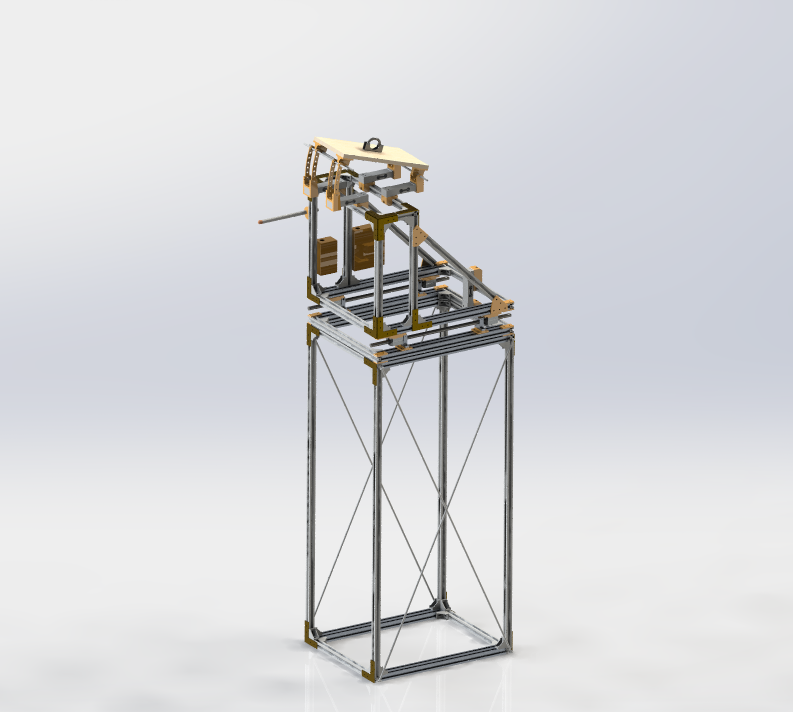
\includegraphics[width=.8\linewidth]{figuras/renders/perspectiva_sem_asa_com_pitot.png}
    \caption{Renderização da bancada modelada no software Solidworks 2016\cite{autor}.}
    \label{fig:placeholder}
\end{figure}

\begin{figure}[!ht]
    \centering
    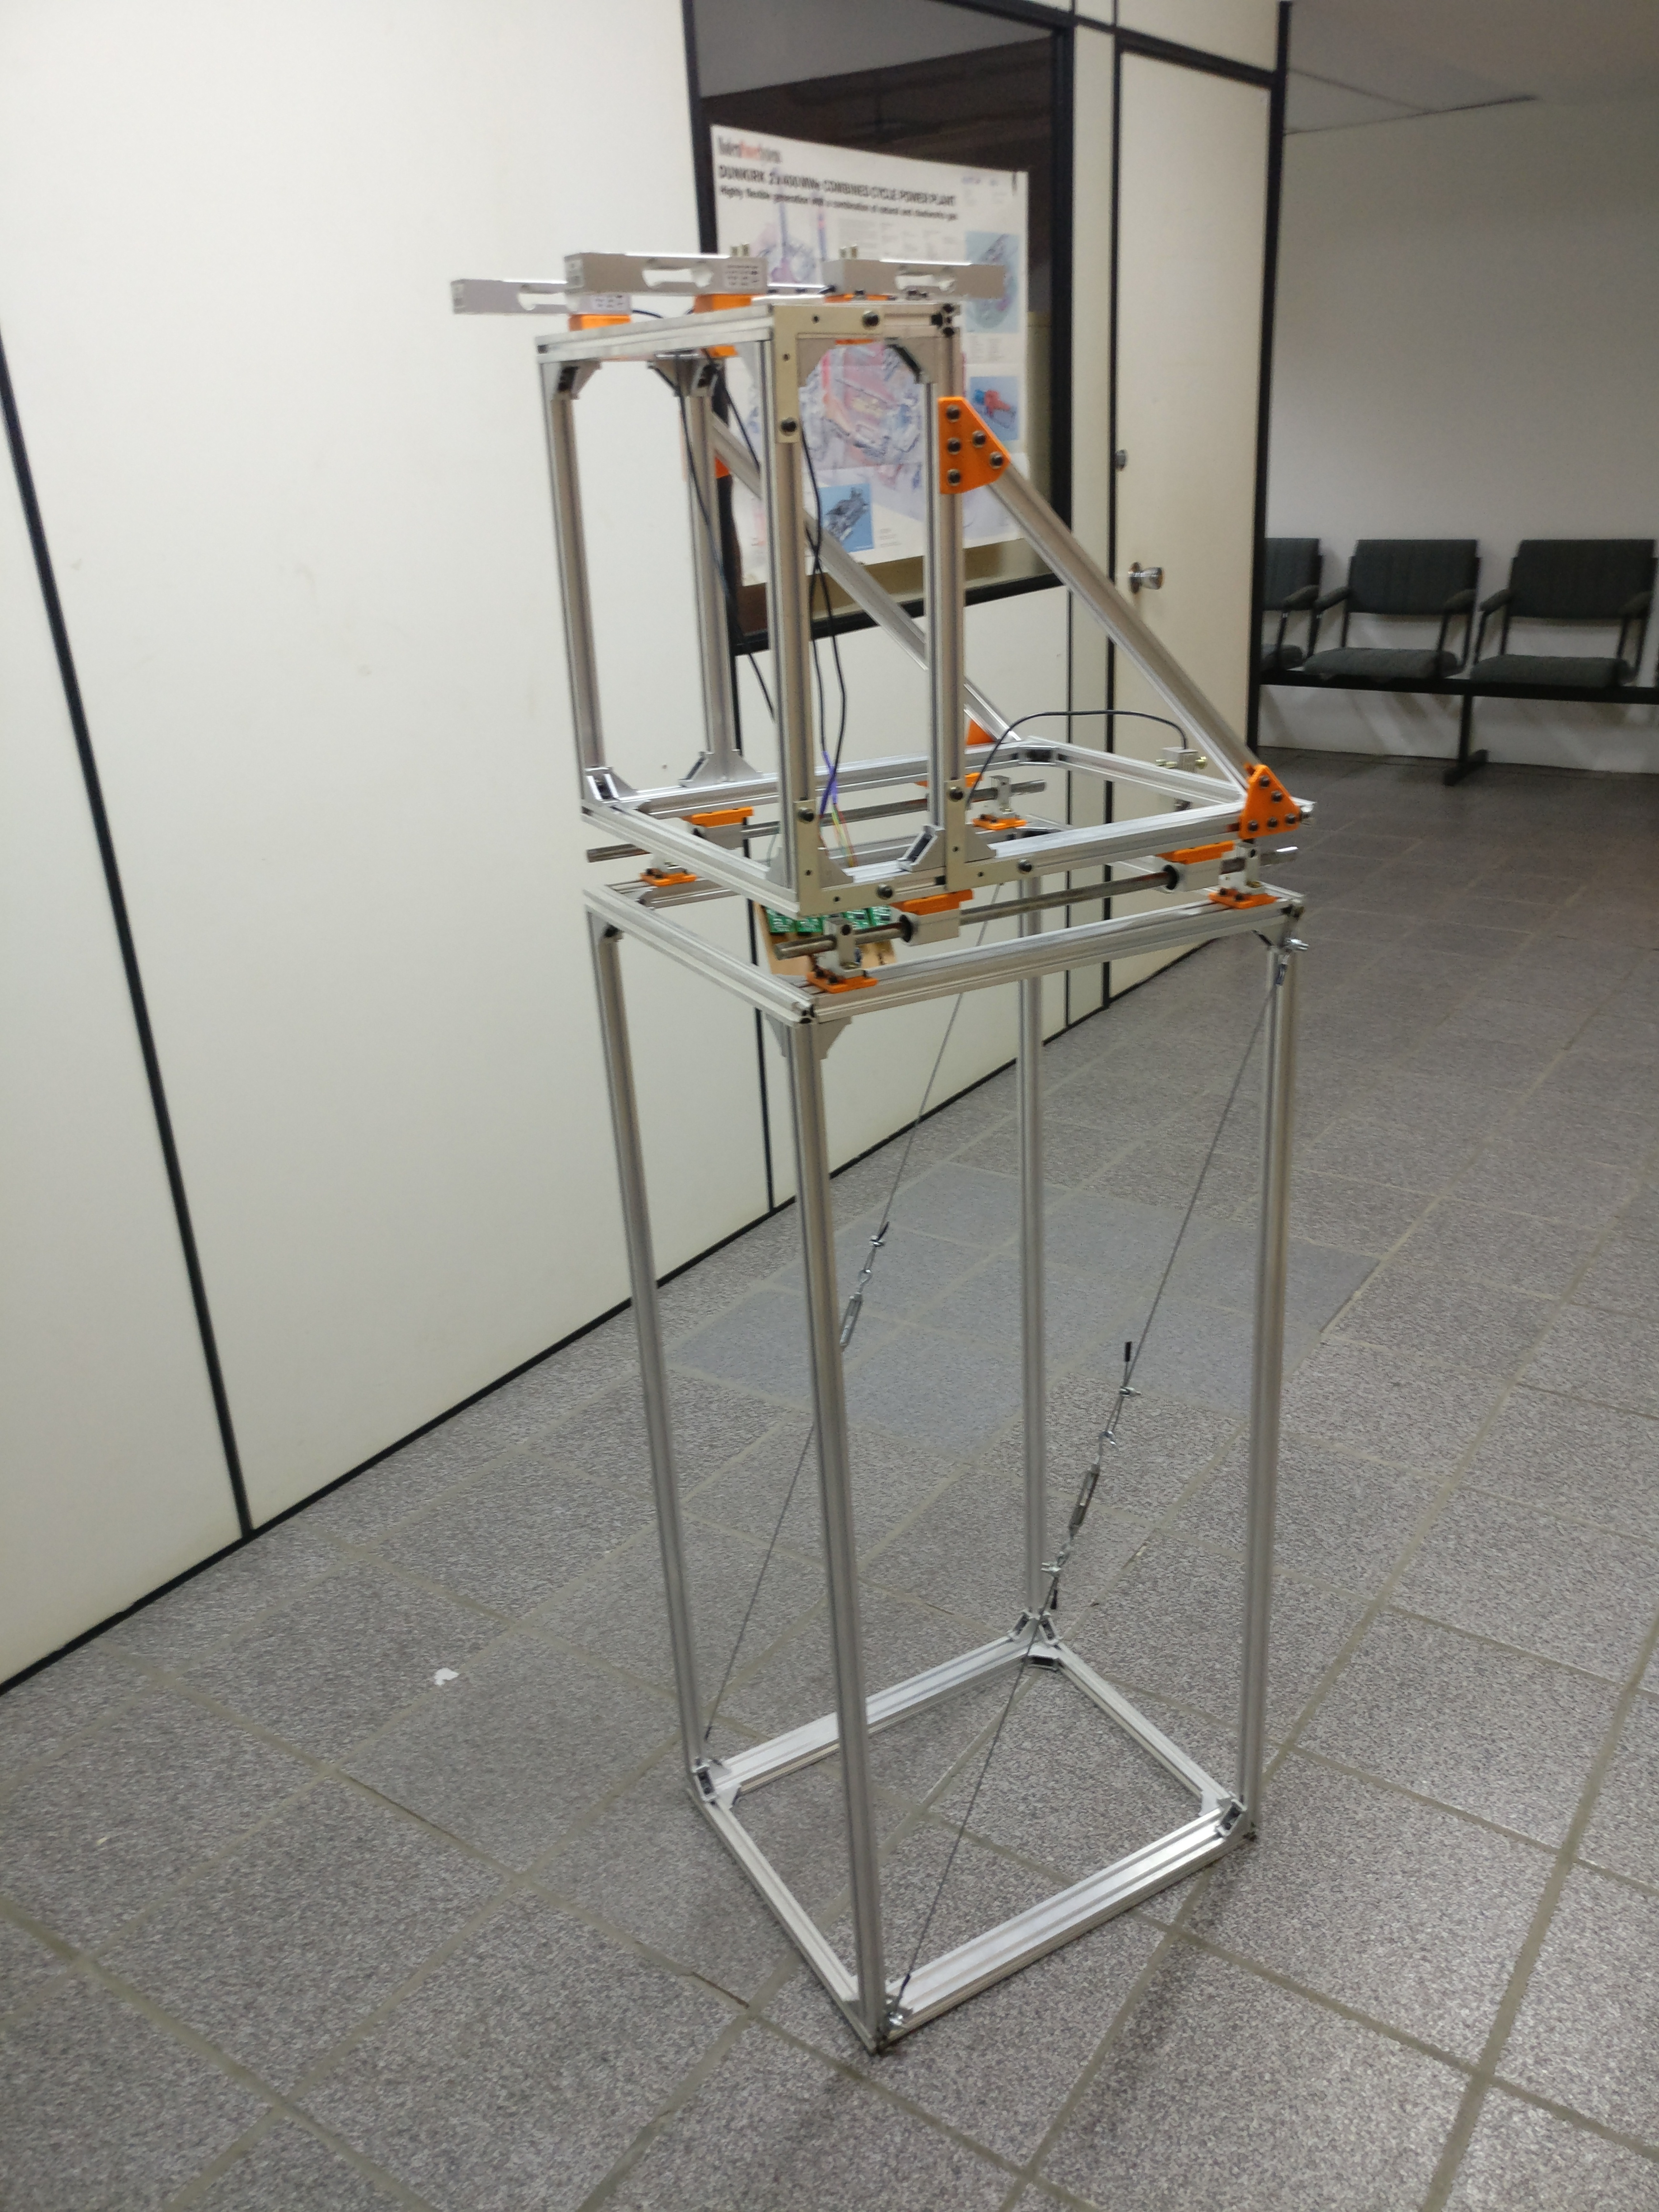
\includegraphics[width=.8\linewidth]{figuras/construcao/bancada_inteira.jpg}
    \caption{Foto da bancada construída\cite{autor}.}
    \label{fig:placeholder}
\end{figure}

A proposta deste trabalho consiste no projeto e análise de uma bancada para medição de esforços aerodinâmicos sem túnel de vento, a ser utilizada para a caracterização aerodinâmica de componentes de VANTs. Tal bancada consiste de células de carga, tubos de pitot e outros sensores, e é embarcada em um veiculo automotor, que ao ser movimentado faz com que um escoamento surja sobre o componente a ser experimentado.

\section{Objetivo geral}

Desenvolvimento de uma bancada de baixo custo para caracterização aerodinâmica de componentes de VANTs, visando a eliminação ou minimização da necessidade de um túnel de vento.
 % Texto do cap1.tex
\chapter{Revisão de Literatura}\label{chp:rev}

Bancada semelhante já foi construída pela NASA para estudos aerodinâmicos da aeronave LEAPtech [6], e seus resultados comparados aos simulados em computador [7].


\begin{itemize}
    \item Revisao de aerodinamica
    \item Revisao de metrologia
    \item Projeto Bancada 1.0
\end{itemize} % Texto do cap2.tex
\chapter{Metodologia}\label{chp:met}

\section{Projeto}

\subsection{Necessidades}

\subsubsection{O cliente}
O cliente do presente projeto é a equipe Céu Azul Aeronaves, que representa anualmente a UFSC na competição SAE Brasil Aerodesign. A equipe desenvolve VANTs com missões variadas, mas que (em geral) giram em torno da maximização da eficiência estrutural da aeronave projetada \citep{brasil2018sae}. O autor. do presente texto trabalhou durante 5 anos na equipe e viu nesta necessidade a oportunidade de desenvolvimento do presente trabalho.

O objetivo da bancada é medir os coeficientes aerodinâmicos (de sustentação, arrasto e momento) em componentes dos VANTs desenvolvidos na equipe, além da medição de empuxo dinâmico em conjuntos moto-propulsores e a interação de seu escoamento com o restante da aeronave.

Para cumprir com o objetivo proposto, algumas necessidades foram levantadas:

\begin{enumerate}
    \item Tal bancada deve possuir rigidez suficiente para que suas medições sejam consistentes no tempo e a necessidade de manutenção seja baixa.
    \item Deve ser possível acoplar a bancada na caçamba de uma camionete ouO autor ao rack de um carro comum, de modo a facilitar sua instalação.
    \item Levando em conta que a equipe sofre de alta rotatividade de membros e nem sempre é possível garantir que existirão pessoas capacitadas a trabalhar neste projeto é importante que a bancada em questão seja entregue na forma de um "produto final", isto é, funcione sem a necessidade de conhecimento de suas intrinsidade, com pouco mais que um manual de instruções e considerações para seu uso.
    \item Da mesma forma que o uso da bancada deve ser facilitado, também deve ser assim o uso dos dados fornecidos por ela. Idealmente se deseja que a mesma entregue os coeficientes finais, já processados, assim como suas incertezas de medição.
\end{enumerate}

\subsection{Considerações}

Assume-se para o presente projeto que o escoamento de ar que alcança a geometria analisada tem direção relativamente estável, é aproximadamente paralela ao deslocamento do veiculo e que a velocidade é praticamente constante para pequenos trechos.

Dado que a velocidade do veiculo é controlada por um piloto humano, estima-se que oscilações da ordem de 10\% na velocidade são esperadas durante os patamares de velocidade e serão mensuradas através de tubos de Pitot. Durante as análises dos resultados esta estimativa foi validada.

\begin{figure}[!ht]
    \centering
    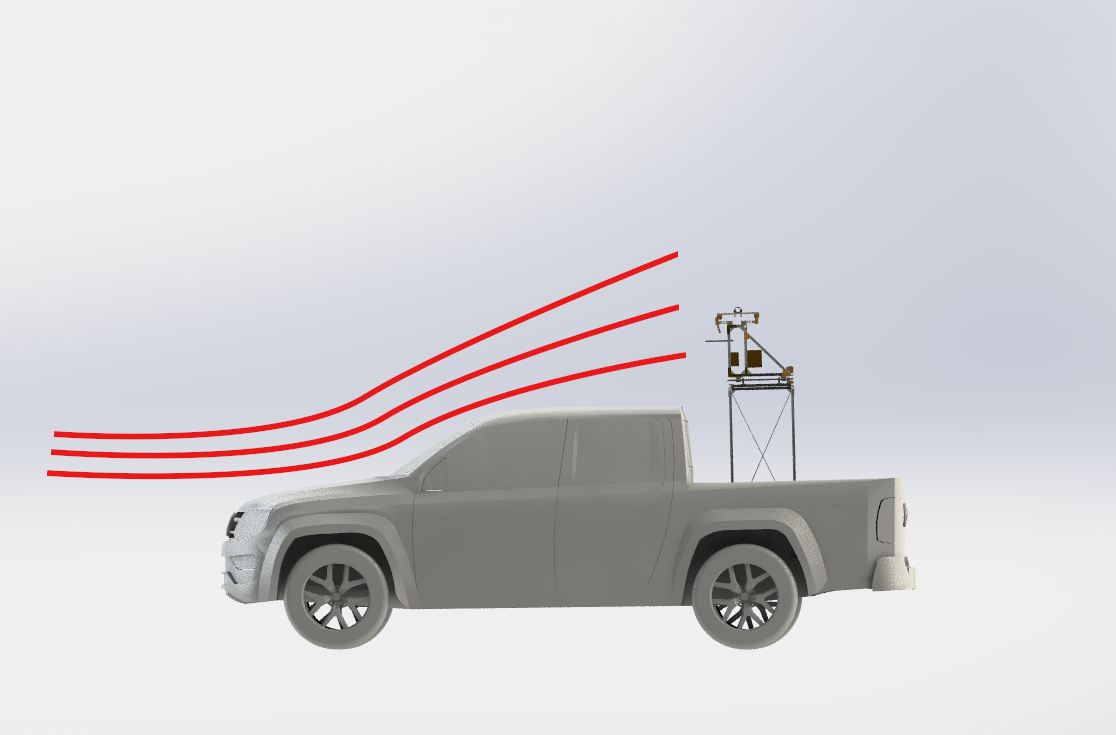
\includegraphics[width=.8\linewidth]{figuras/renders/bancada_no_carro_lateral_induzido.png}
    \caption{Ângulo de escoamento induzido pela carenagem do carro sobre a região de medições. Fonte: O autor.}
    \label{fig:vehicle-angle}
\end{figure}

É possível também que a carroceria do veiculo induza um angulo diferente de zero ao escoamento que chega a bancada (ver figura \ref{fig:vehicle-angle}). Um Pitot de múltiplas tomadas sera instalado na bancada a fim de medir este angulo e ajustar os dados no pós-processamento. Eh importante ressaltar que tal sonda  possui limitação de operação de aproximadamente 15 graus em cada sentido \citep{azartash2017evaluation}, sendo assim, ângulos maiores que este não terão uma leitura adequada. Grandes desvios de angulo do escoamento ou velocidades muito instáveis provavelmente tornarão os resultados do teste inválidos e portanto cuidados devem ser tomados para que o teste se conduza de forma adequada.

\begin{figure}[!ht]
    \centering
    \caption{Situações adversas não compreendidas pelo modelo e que devem ser prevenidas durante o teste. Fonte: O autor.}
        \subfloat[Surgimento de força radial sob o componente quando em curva.]{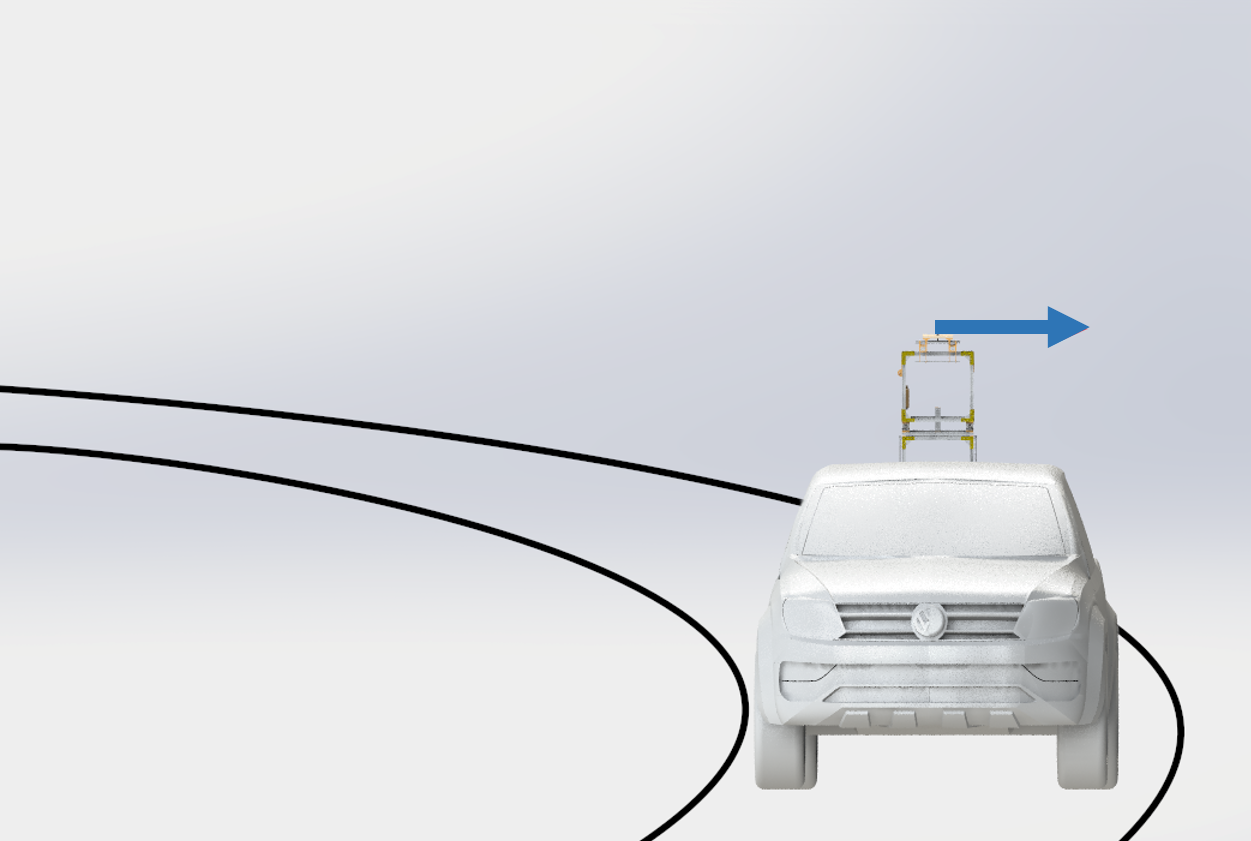
\includegraphics[width=0.4\columnwidth]{figuras/renders/bancada_no_carro_curva_frontal_forca.png}}
        \label{forca_radial_frontal}
        \qquad
        \subfloat[Momento de rolagem artificial medido quando em curva.]{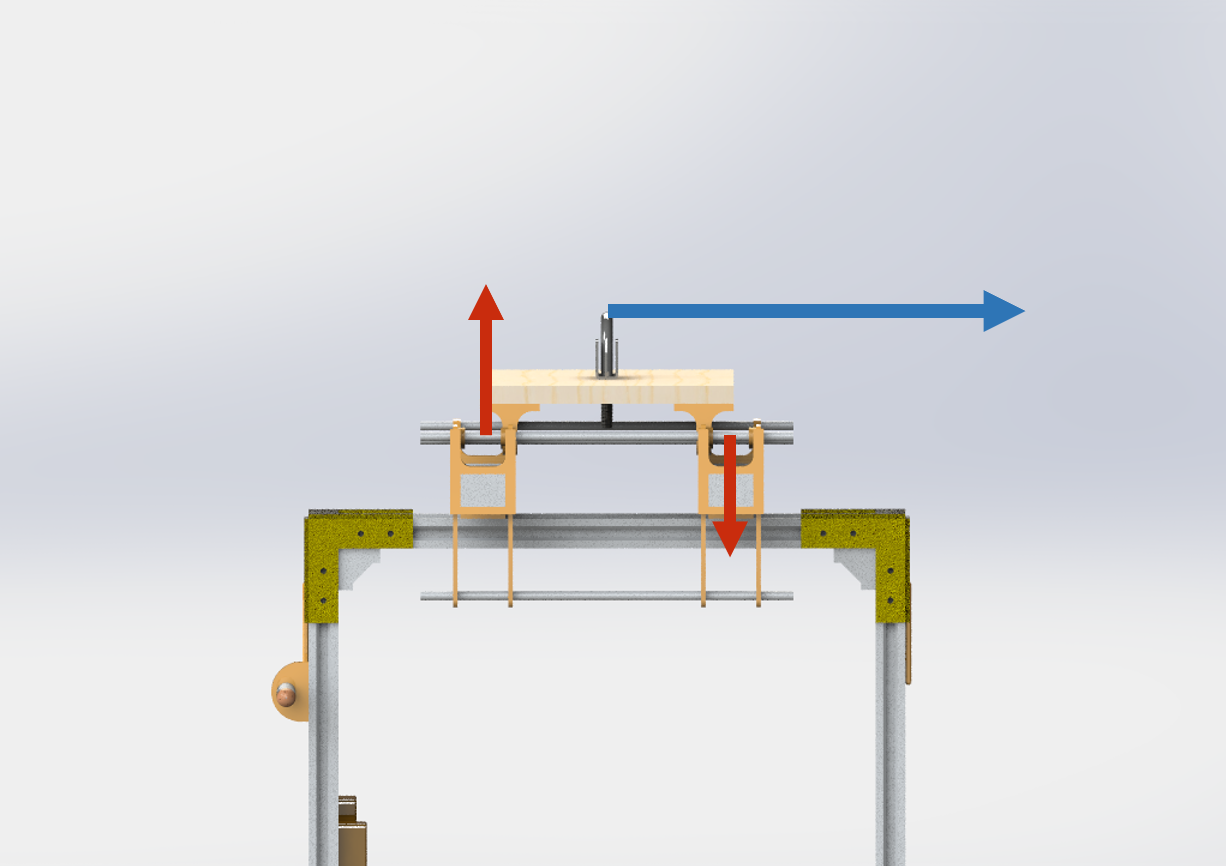
\includegraphics[width=0.4\columnwidth]{figuras/renders/carro_momento_roll_frontal_forca.png}}
        \label{momento_falso_roll}
        % \qquad
        % \subfloat[Oscilações em pista causam erro na medição das forças e desalinhamento do escoamento.]{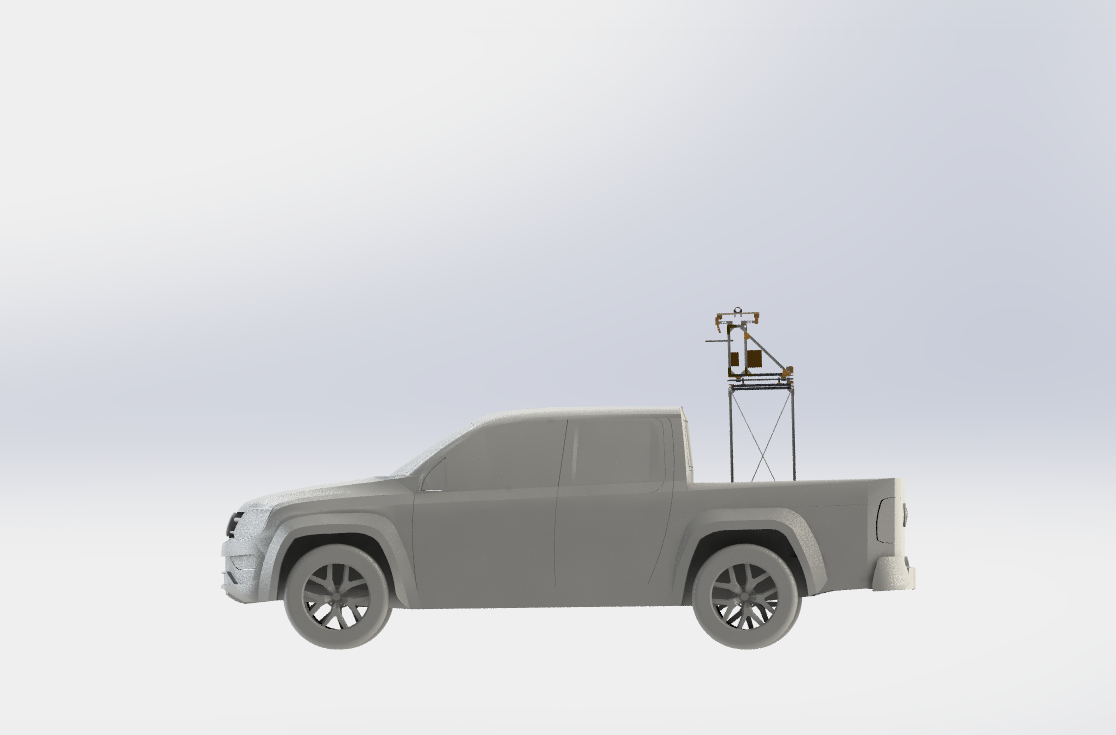
\includegraphics[width=0.4\columnwidth]{figuras/renders/bancada_no_carro_lateral.png}}
        % \label{ocsilacoes_em_pista}
\end{figure}

Assume-se também que existem obstáculos na pista (tais como buracos e pequenas elevações), mas que de forma geral o teste será conduzido em pistas retas, planas e com poucos buracos, de modo que não existam grandes vibrações ou acelerações radiais a serem modeladas no sistema. Pequenas oscilações serão medidas por acelerômetros e giroscópios e levadas em conta também no pós-processamento.

\subsection{Estimativas}

Para os projetos mecânico e eletrônico foram estimadas situações extremas de medição e para estas a bancada foi dimensionada:

\begin{itemize}
    \item Caracterização de aeronave completa com até 300 N de sustentação, 50 N de arrasto e 50 N.m de momento
    \item Caracterização de conjunto motopropulsor com até 70 N de empuxo estático
    \item Escoamentos com velocidade de até 25 m/s
    \item Fatores de carga na bancada de até 4 g
\end{itemize}

\subsection{Solução proposta}

A solução proposta consiste em uma bancada sensoriada, montada sobre uma estrutura metálica que a eleve até a altura desejada para o teste.

O veiculo a ser utilizado nos testes é do modelo Volkswagen Amarok 2017, tendo a caçamba uma altura de 0,8 m e o teto do carro elevando-se 0,9 m acima da altura da caçamba.

\begin{figure}[!ht]
    \centering
    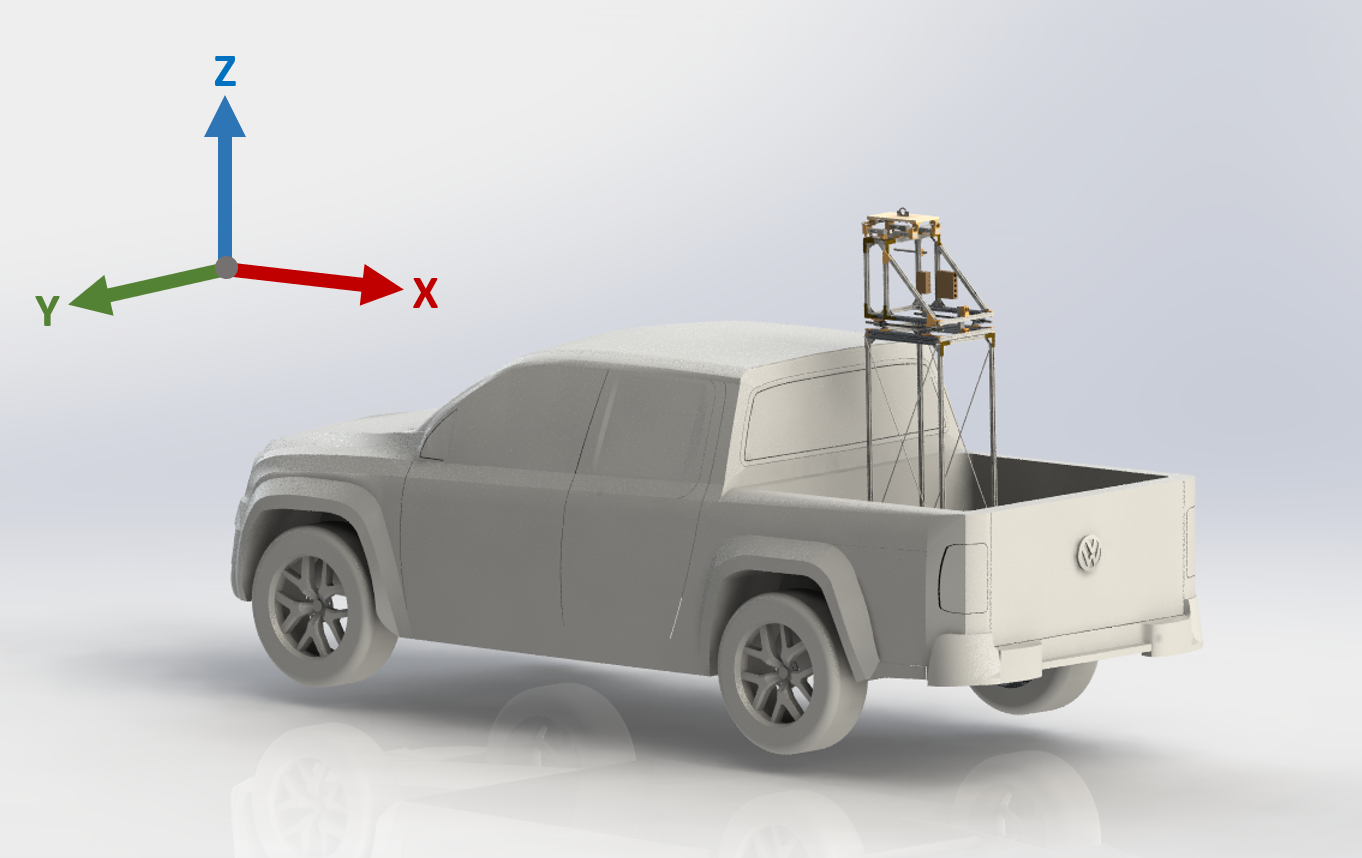
\includegraphics[width=.8\linewidth]{figuras/renders/bancada_no_carro_perspectiva_eixos.png}
    \caption{Bancada proposta instalada no veiculo, com eixos de referencia utilizados neste trabalho. Fonte: O autor.}
    \label{fig:placeholder}
\end{figure}

\subsubsection{Sensoriamento das forças}

As forças verticais na bancada são sensoriadas por quatro células de cargas enquanto a força horizontal é medida por uma quinta célula de carga. A célula horizontal permite medição do arrasto/empuxo, o somatório das células verticais permitem a medição da sustentação, a diferença entre as células frontais e traseiras permite a medição do momento de picada (momento ao redor do eixo Y) e a diferença entre as células da esquerda e da direita permite a medição do momento de rolagem (momento ao redor do eixo X).

\begin{figure}[!ht]
    \centering
    \caption{Formas de leitura das diferentes cargas na balança da bancada. Fonte: O autor.}
        \subfloat[Leitura de sustentação.]{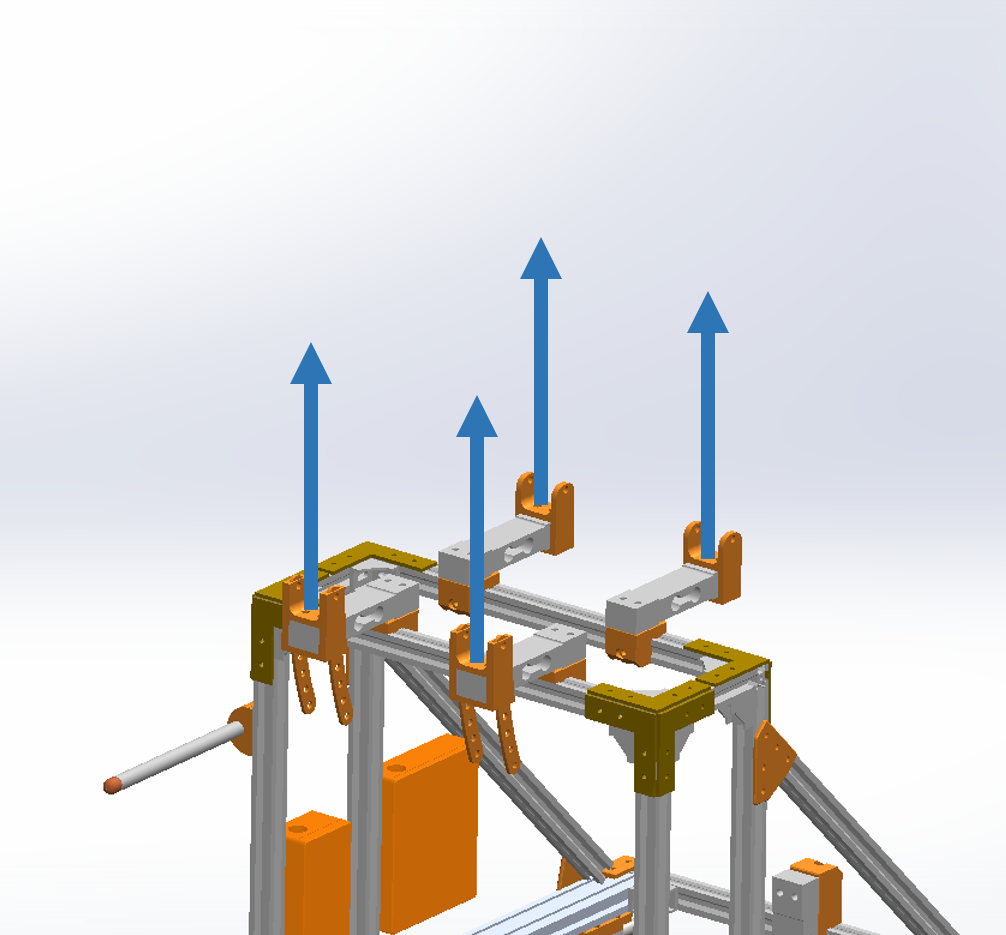
\includegraphics[width=0.4\columnwidth]{figuras/renders/esquematico_celulas_lift_forcas.png}}
        \label{leitura_sustentacao}
        \qquad
        \subfloat[Leitura de arrasto.]{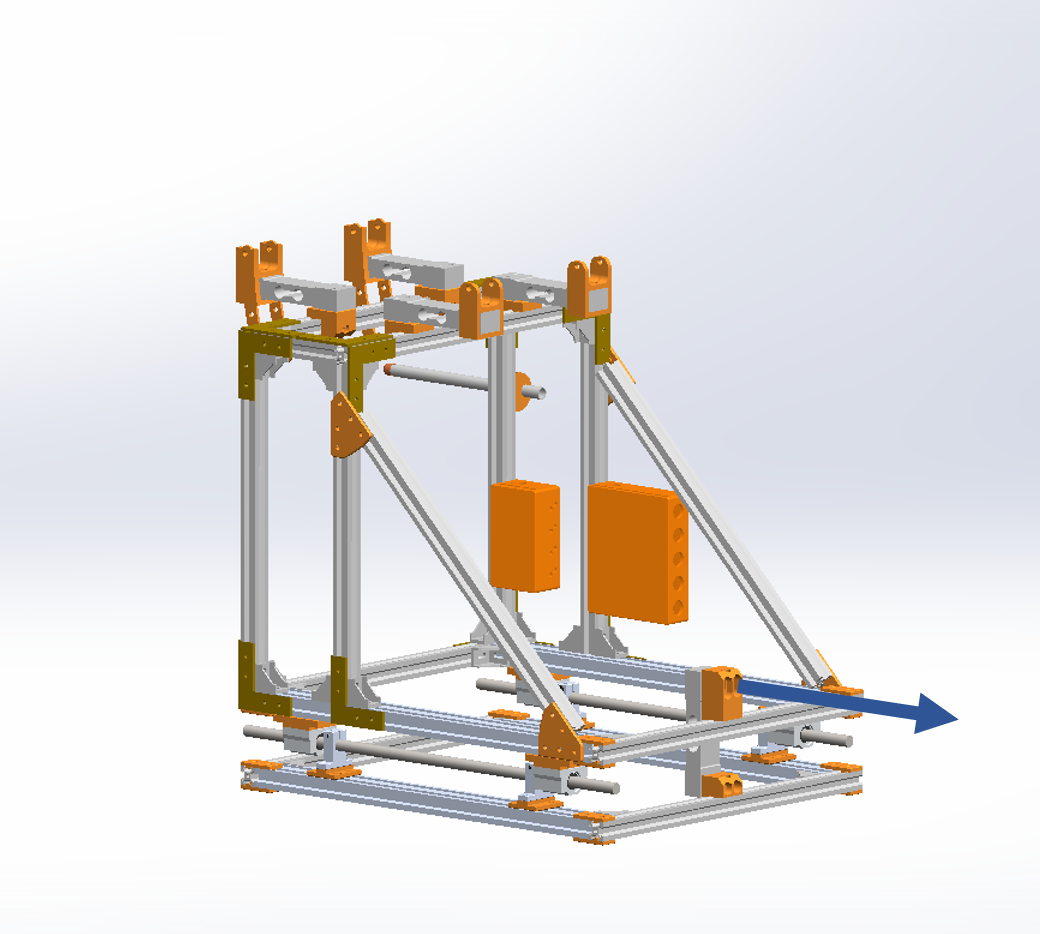
\includegraphics[width=0.4\columnwidth]{figuras/renders/esquematico_celulas_drag_2_forca.png}}
        \label{leitura_arrasto}
\end{figure}

\begin{figure}[!ht]
    \centering
    \caption{Formas de leitura das diferentes cargas na balança da bancada. Fonte: O autor.}
        \subfloat[Leitura de momento de picada.]{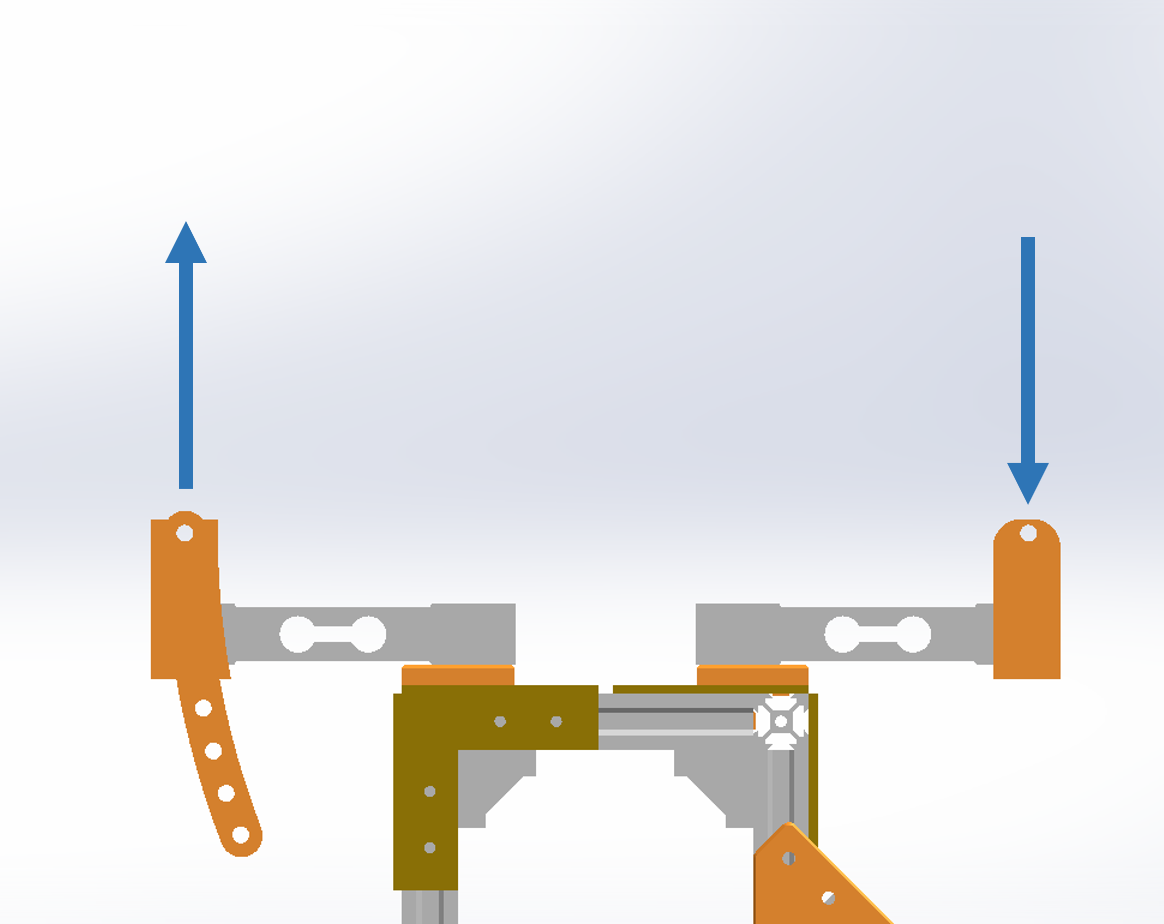
\includegraphics[width=0.4\columnwidth]{figuras/renders/esquematico_celulas_momento_pitch_forcas.png}}
        \label{leitura_momento_pitch}
        \qquad
        \subfloat[Leitura de momento de rolagem.]{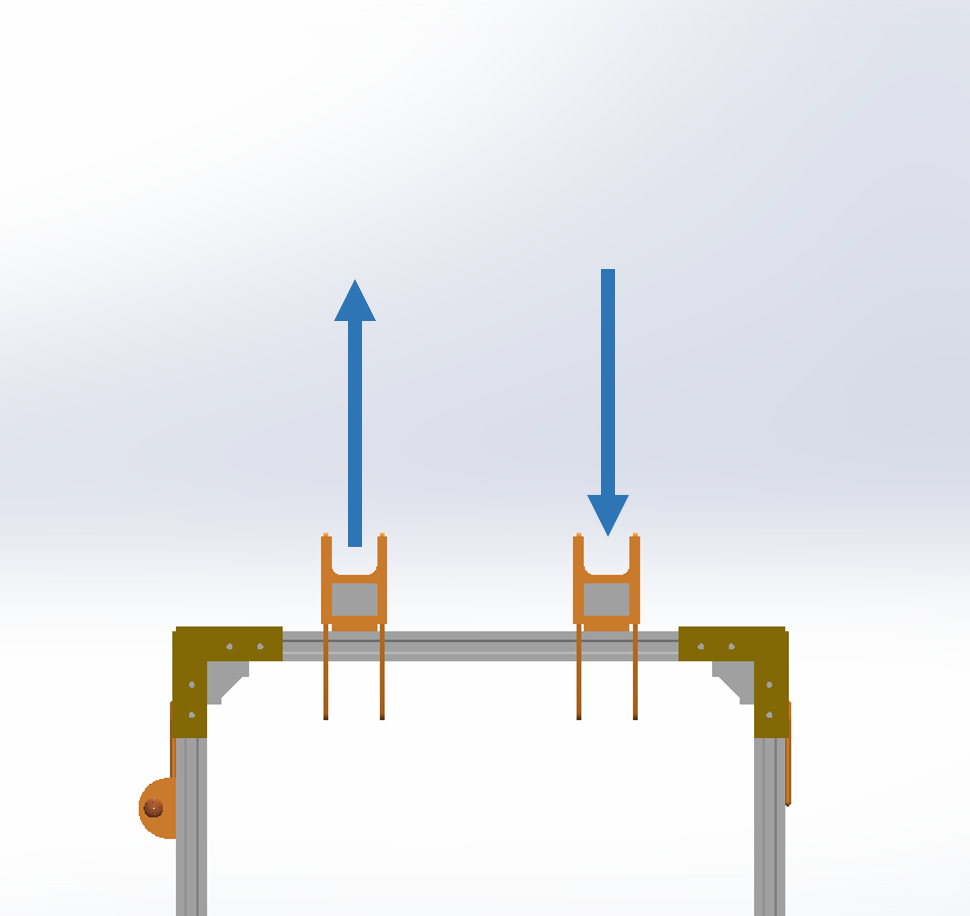
\includegraphics[width=0.4\columnwidth]{figuras/renders/esquematico_celulas_momento_roll_2_forcas.png}}
        \label{leitura_momento_roll}
\end{figure}

\subsubsection{Sensoriamento de velocidade e ângulo de ataque}

Ainda na bancada serão instalados um tubo de Pitot e um Pitot de múltiplas tomadas (sonda de angulo de ataque). Ambos serão instalados o mais próximo possível ao escoamento livre. Enquanto o Pitot será acoplado à própria bancada, a sonda ficará alinhada com o eixo de referencia em pitch do componente a ser analisado, de modo a medir o angulo de ataque real do mesmo. 

\begin{figure}[!ht]
    \centering
    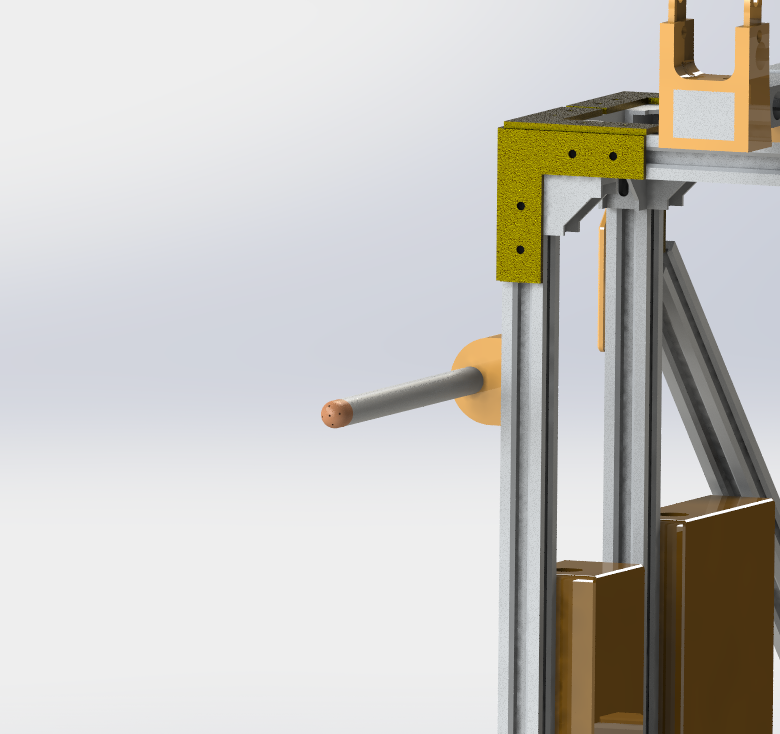
\includegraphics[width=.4\linewidth]{figuras/renders/detalhe_pitot_bancada.png}
    \caption{Posicionamento do tubo de Pitot na bancada para medição da velocidade de fluxo livre . Fonte: O autor.}
    \label{fig:placeholder}
\end{figure}

\begin{figure}[!ht]
    \centering
    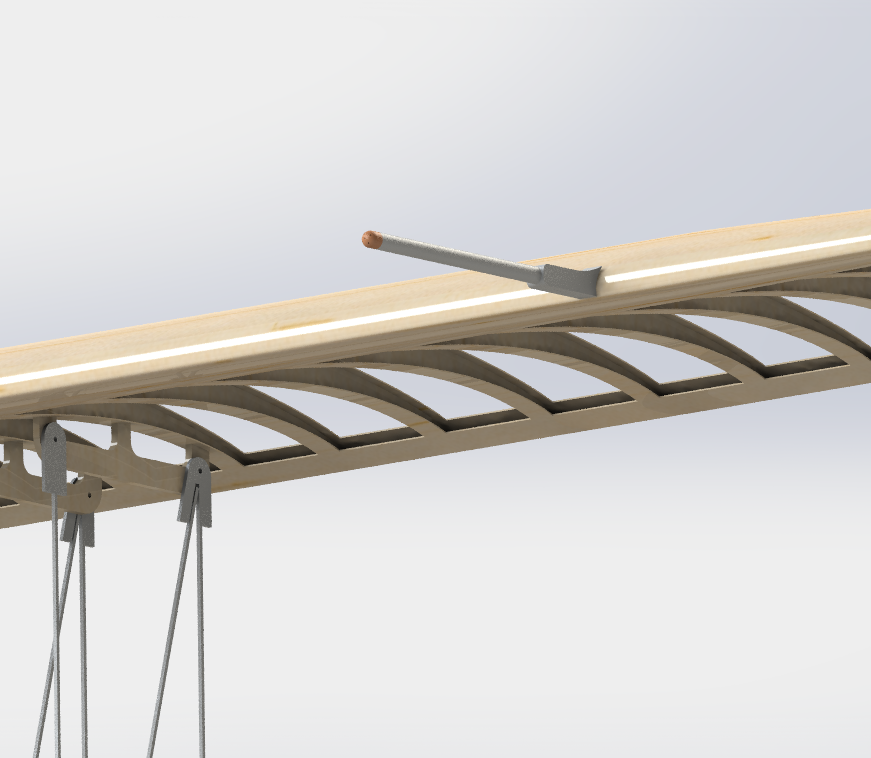
\includegraphics[width=.5\linewidth]{figuras/renders/sonda_aoa_asa_superior.png}
    \caption{Detalhe do Pitot de múltiplas tomadas (sonda de angulo de ataque) montada na asa superior da aeronave testada. Fonte: O autor.}
    \label{fig:pitot_asa}
\end{figure}

O sistema deve comportar ainda a adição de novos sensores de forma a permitir a caracterização do escoamento em outros pontos de interesse, como esteira da hélice ou escoamento incidente no profundor.

\subsubsection{Sensoriamentos adicionais}

Para a medição do fator de carga vertical, assim como da temperatura e pressão do ar, uma Unidade de Medição Inercial (IMU) com acelerômetro, giroscópio, barômetro e termômetro será instalada na bancada.

\begin{figure}[!ht]
    \centering
    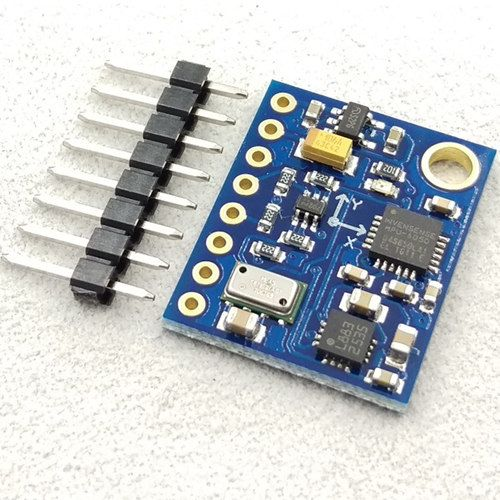
\includegraphics[width=.5\linewidth]{figuras/internet/IMU.jpg}
    \caption{Unidade de Medição Inercial (IMU) utilizada na bancada. Fonte: O autor.}
    \label{fig:imu}
\end{figure}

\subsubsection{Estação de controle e software de processamento}

Num primeiro momento foi levantada a possibilidade de se utilizar um computador portátil como estação de controle da bancada. Avaliou-se porém que isto poderia tornar o uso dificultado, já que em geral estes computadores possuem baterias que permitem poucas horas de uso continuo, limitando o tempo de execução de teste, além de serem pouco práticos de se utilizar dentro do carro.

De forma a facilitar o uso da bancada todo o controle do sistema foi projetado para ser realizado através de um aplicativo para celular, mostrado nas figuras \ref{tela_app1} e \ref{tela_app3}. Nele é possível controlar a execução do teste, inserir informações para posterior avaliação, assim como acompanhar as medições dos sensores em tempo real, de modo a identificar possíveis problemas de forma rápida.

\begin{figure}[!ht]
    \centering
    \caption{Telas do aplicativo de controle da bancada. Fonte: O autor. e Mariga(2018)}
        \subfloat[Tela inicial do aplicativo, permitindo escolher entre o uso dos sensores do celular ou a estação de controle da telemetria]{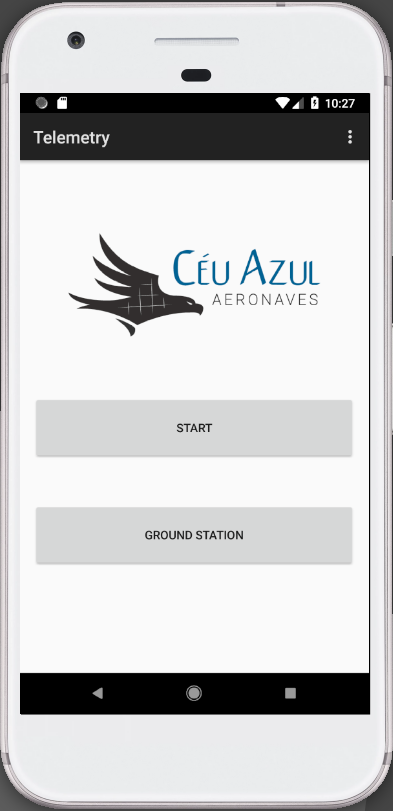
\includegraphics[width=0.3\columnwidth]{figuras/app/app1.png}}
        \label{tela_app1}
        \qquad
        \subfloat[Tela de conexão do radio de telemetria.]{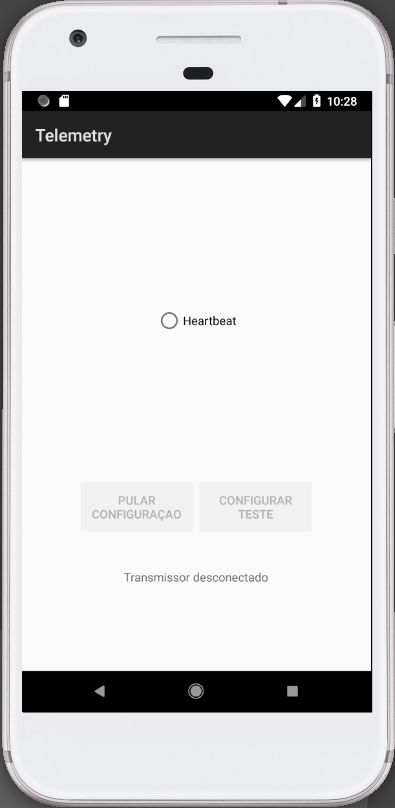
\includegraphics[width=0.3\columnwidth]{figuras/app/app2.png}}
        \label{tela_app2}
\end{figure}

\begin{figure}[!ht]
    \centering
    \caption{Telas do aplicativo de controle da bancada. Fonte: O autor. e Mariga(2018)}
        \subfloat[Tela de configuração do teste.]{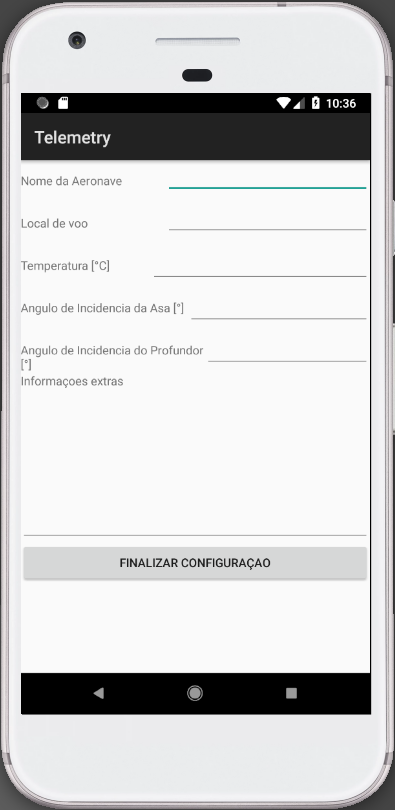
\includegraphics[width=0.3\columnwidth]{figuras/app/app3.png}}
        \label{tela_app3}
        \qquad
        \subfloat[Tela de controle do teste. Nesta tela o responsável pelo teste pode iniciar, pausar e finalizar a gravação e transmissão dos dados, zerar algumas variáveis a visualizar os dados fornecidos pela bancada.]{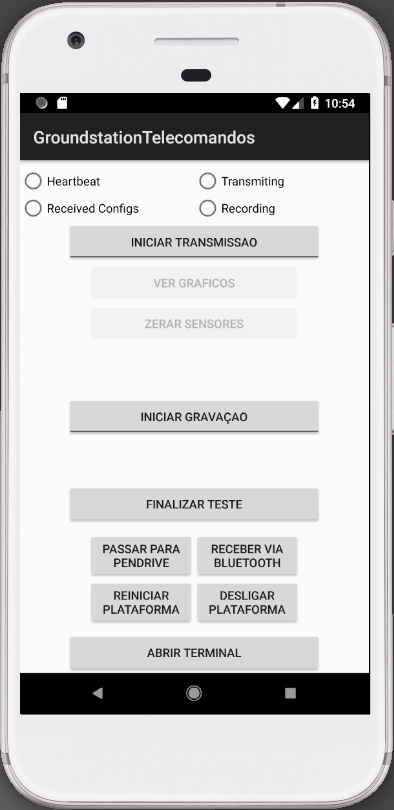
\includegraphics[width=0.3\columnwidth]{figuras/app/app4.png}}
        \label{tela_app4}
\end{figure}

Será desenvolvido ainda um software de tratamento e analise de dados com interface gráfica e uso facilitado, este a ser utilizado em computador, devido a maior flexibilidade do mesmo para a análise de dados, que demanda mais tempo.

\section{Projeto Mecânico}

Para o projeto mecânico foram levantadas as seguintes necessidades:

\begin{itemize}
    \item Facilidade construtiva, de forma a tornar rápida a construção e manutenção da bancada
    \item Baixo peso, de modo a não se criar uma barreira quanto ao uso da mesma
    \item Baixo arrasto aerodinâmico, a fim de diminuir a influência da estrutura nas medições
    \item Rigidez, para que as forças e momentos medidos sejam correspondentes aos modelados
    \item Baixo custo
\end{itemize}

Uma solução que responde de forma positiva à maioria dessas necessidades é a de uma estrutura composta de perfis extrudados de alumínio (figura \ref{fig:perfil_aluminio}). Este tipo de estrutura é comumente encontrada em laboratórios ou fábricas, sendo utilizada para a construção de bancadas experimentais e estações de trabalho.

\begin{figure}[!ht]
    \centering
    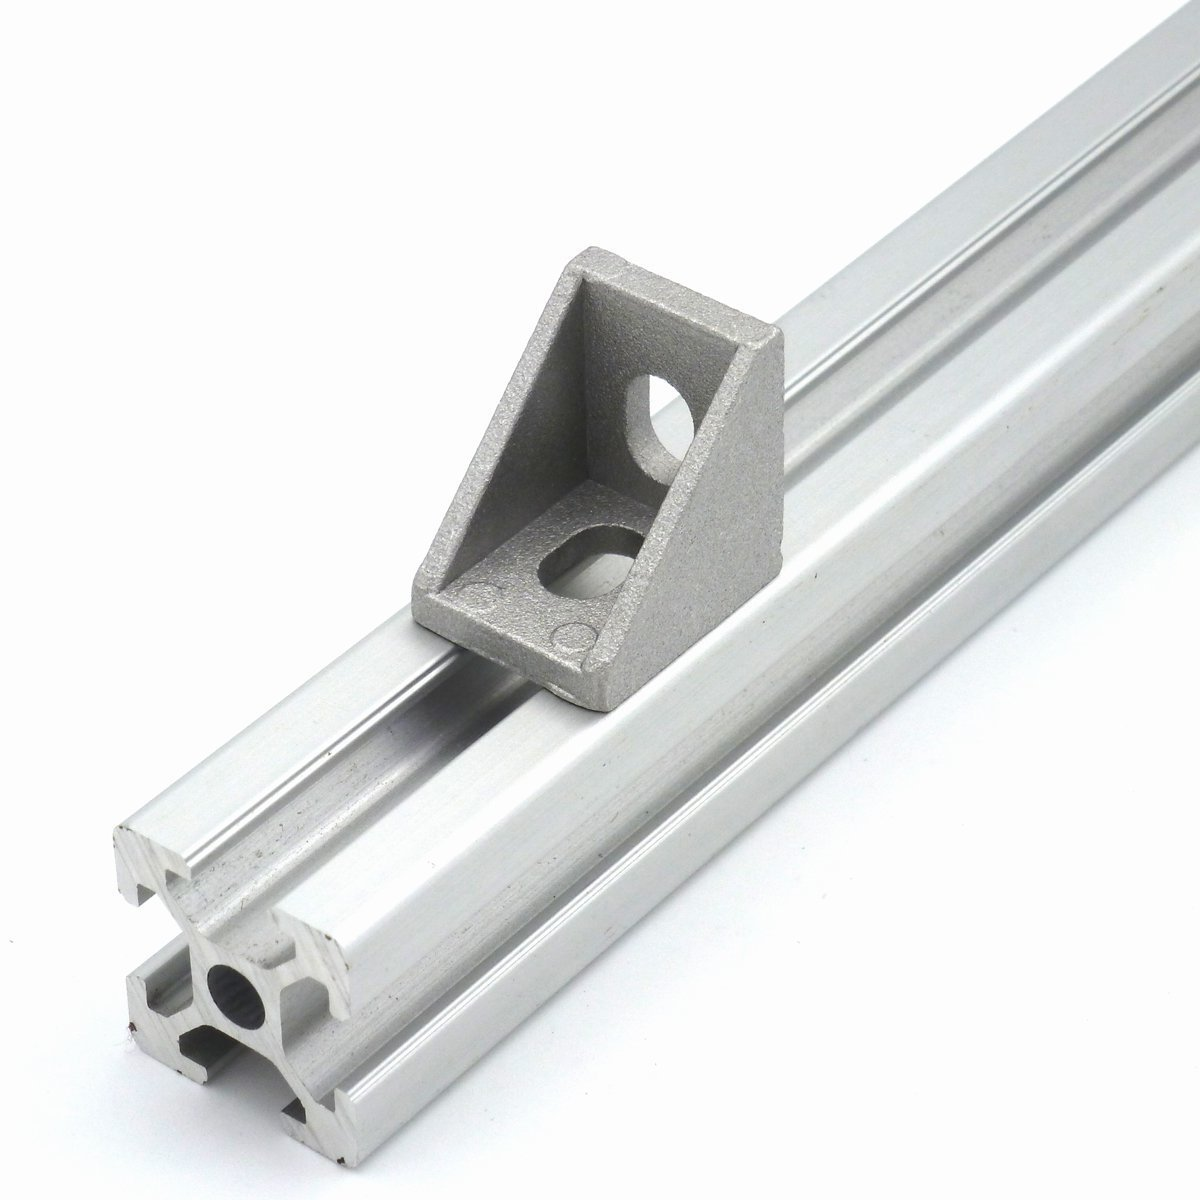
\includegraphics[width=.4\linewidth]{figuras/internet/perfil_aluminio.jpg}
    \caption{Perfil extrudado em alumínio utilizado na construção da bancada. Fonte: O autor.}
    \label{fig:perfil_aluminio}
\end{figure}

A desvantagem desta estrutura fica no provável alto arrasto aerodinâmico. Este porém é um problema contornável posteriormente carenando-se a estrutura. Ainda assim, com ou sem carenagem, este arrasto deve ser levado em conta nos testes e a maneira levantada de se mensurar esta grandeza é realizar os testes sem um componente a ser medido, medindo-se assim o arrasto aerodinâmico da própria bancada para que se possa descontar este valor das medições posteriores.

De modo a se medir o arrasto, duas soluções foram consideradas: 

\begin{enumerate}
    \item Uma célula de carga horizontal, tendo a bancada liberdade de movimento no eixo X (figura \ref{bandeja_inferior_1}a)
    \item Três células de carga restringindo completamente os graus de liberdade da bancada(figura \ref{bandeja_inferior_1}b)
\end{enumerate}

\begin{figure}[!ht]
    \centering
    \caption{Soluções para a medição de arrasto na bancada. Fonte: O autor.}
        \subfloat[Solução utilizando apenas uma célula de carga.]{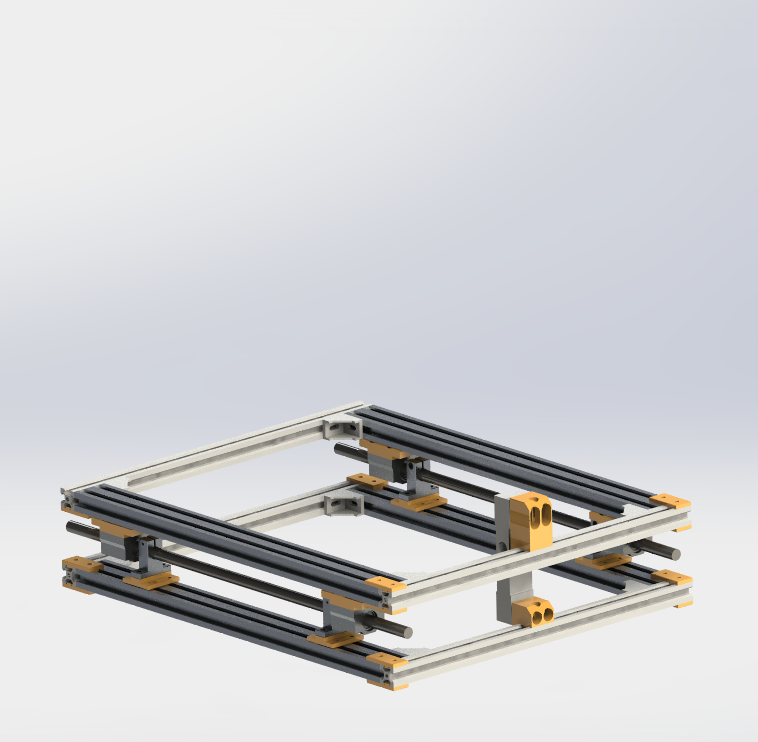
\includegraphics[width=0.4\columnwidth]{figuras/renders/bandeja_inferior_2.png}}
        \label{bandeja_inferior_1}
        \qquad
        \subfloat[Solução utilizando três células de carga.]{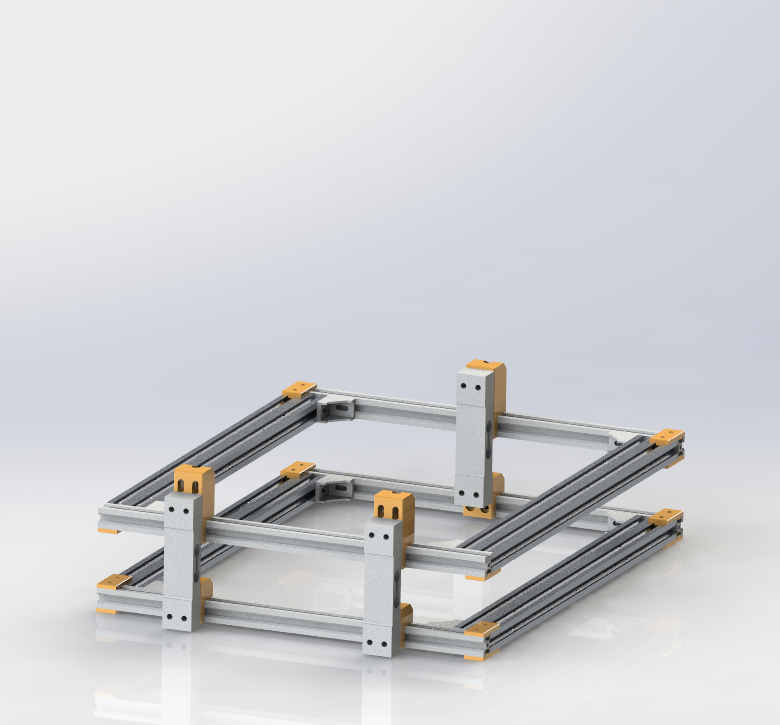
\includegraphics[width=0.4\columnwidth]{figuras/renders/bandeja_inferior_3.png}}
        \label{bandeja_inferior_2}
\end{figure}

Devido ao fato de que a segunda solução exigiria ao menos três células de carga e as colocaria como componentes estruturais (já que não existiria outra ligação estrutural entre a parte inferior e superior da bancada) a primeira opção foi escolhida.

Para dar liberdade de movimentação no eixo X um conjunto de guias lineares e fixações rolamentadas foi escolhido, devido a seu baixo atrito e baixo custo. A desvantagem desta solução com apenas uma célula de carga se da justamente devido a existência desta força de atrito das guias no eixo X, que a principio não é medida. Esta força pode porem ser avaliada num primeiro momento, em laboratório, e compensada posteriormente.
    
\section{Projeto Eletrônico}

Para o sistema eletrônico da bancada tomou-se como ponto de partida a telemetria T2016, desenvolvida pela equipe Céu Azul inicialmente para utilização nos projetos da classe Advanced.

Tal sistema consiste de um computador central, modelo Raspberry Pi 3 B+, rodando um sistema operacional Linux, com sensores conectados como periféricos. Entre os sensores já disponíveis na equipe estavam:

\begin{itemize}
    \item Tubos de Pitot com transdutores MPVX7002DP
    \item Modulo GNSS modelo uBlox NEO-6M
    \item IMU modelo GY-86, com acelerômetro de 3 eixos, giroscópio de 3 eixos, magnetômetro de 3 eixos, barômetro e termômetro
\end{itemize}

Além destes sensores o sistema possui um par de rádios seriais de 433MHz, que pode ser utilizado para transmissão dos dados em tempo real para o celular, comunicando a bancada com o aplicativo controlado pelo operador.

Para a medição das forças na bancada foi necessária a aquisição de células de carga e transdutores de célula de carga. Devido ao baixo custo optou-se por células sem marca. Esta decisão implica contudo num custo extra de tempo para a caracterização das células.

Para a transdução dos dados das células de carga foram adquiridos módulos HX711. Estes módulos são bastante comuns no mercado e implementam num mesmo CI a alimentação e leitura da ponte de Wheatstone, além da conversão dos dados analógicos em dados digitais. A maior vantagem deste CI é provavelmente a alimentação integrada da ponte de Wheatstone, por ser previamente estabilizada e filtrada, resultando em uma alta relação sinal-ruido. Em geral essa alimentação acontece em circuitos discretos separados do CI de leitura, e acabam resultando numa pior relação sinal-ruido. Este CI permite alimentação entre 2.7V e 5.5V e o conversor analógico-digital (ADC) interno possui resolução de 24bits.

\section{Projeto de Software Embarcado}

O software que roda de forma embarcada na plataforma central consiste em uma serie de módulos escritos em Python com funções desmembradas. Entre as funções necessárias no software destacam-se:

\begin{itemize}
    \item Aquisição de dados dos sensores
    \item Parseamento dos dados para padrão comum
    \item Transmissão serial de dados via radio
    \item Recebimento e interpretação de comandos externos
    \item Gravação dos dados no sistema
    \item Coordenação e sincronia dos processos paralelizados
\end{itemize}

A figura \ref{fig:esquematico_software_embarcado} mostra a arquitetura do software dividida em seus diversos módulos.

\begin{figure}[!ht]
    \centering
    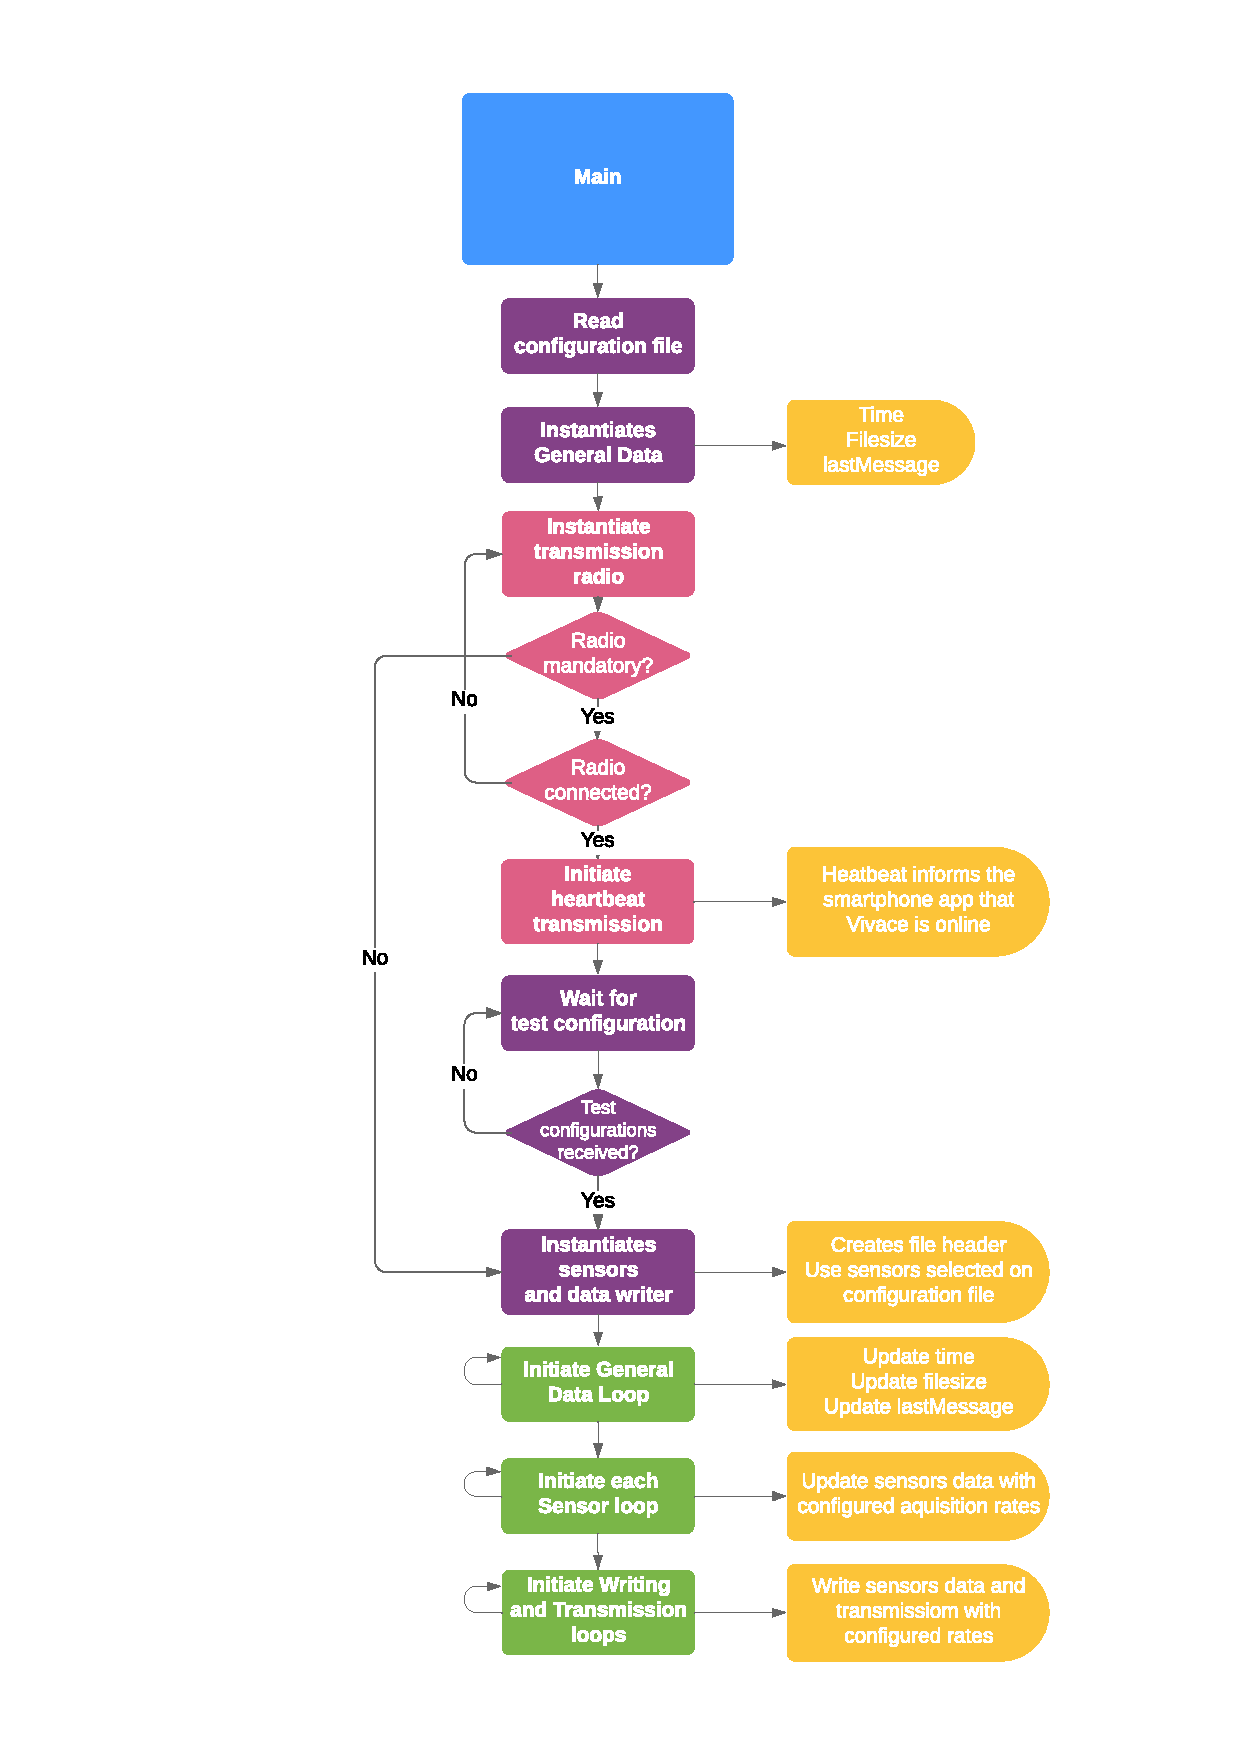
\includegraphics[width=1.0\linewidth]{figuras/diagrams/Vivace_Diagram.pdf}
    \caption{Diagrama de funcionamento do Software embarcado. Fonte: O autor.}
    \label{fig:esquematico_software_embarcado}
\end{figure}

Este software já existia em versão primaria na plataforma T2016 e foi refatorado para uso na nova plataforma, permitindo que suas funções fossem estendidas. A totalidade das mudanças compreendidas por este trabalho pode ser vista no repositório Git do projeto \cite{vivace_2018}.

\section{Projeto do Software de Análise}

O software de análise tem por função receber os dados "crus" gerados pela bancada e entregar dados uteis processados, com suas respectivas incertezas estimadas.

Entre as características desejadas neste software estão:

\begin{itemize}
    \item Apresentar uma interface amigável para uso facilitado
    \item Receber os dados "crus"
    \item Filtrar cada dado conforme especificações previas ou personalizadas pelo usuário
    \item Apresentar os dados crus e processados na forma de gráficos
    \item Permitir interação do usuário com os dados
    \item Exportar os dados em formato útil, seja na forma textual, em planilhas ou mesmo diretamente como gráficos
\end{itemize}

A solução desenvolvida consiste em um software escrito na linguagem Python que responde a todas as necessidades levantadas. 

% A figura \ref{fig:tela_software_analise} mostra a tela principal do software.

% \begin{figure}[!ht]
%     \centering
%     
\includegraphics[width=.8\linewidth]{figuras/outras/placeholder.png}
%     \caption{Tela principal do software de analise. Fonte: O autor.}
%     \label{fig:tela_software_analise}
% \end{figure}

\section{MVP}

Para validar a ideia desta bancada foi proposto um mínimo produto viável (MVP) que possuísse as principais características da solução proposta, mas que pudesse ser construído com materiais já disponíveis pela equipe.

Do ponto de vista de projeto mecânico, esta primeira versão da bancada teve sua estrutura construída em madeira, utilizou corrediças de gaveta para dar liberdade de movimento no eixo X e usava como torre uma estrutura de aço. A escolha por estas soluções se deu pela já disponibilidade das mesmas na equipe Céu Azul.

Do ponto de vista de projeto eletrônico todos os componentes já estavam presentes, com exceção do Pitot de múltiplas tomadas, das células de carga e dos módulos HX711.

Do ponto de vista de software o aplicativo para controle da bancada foi desenvolvido de forma preliminar enquanto o software de tratamento e analise de dados ainda não existia.

As figuras \ref{fig:bancada11}a e \ref{fig:bancada12}b mostram o MVP finalizado.

\begin{figure}[!ht]
    \centering
    \caption{Primeira versão da bancada - MVP. Fonte: Lehmkuhl(2018)}
        \subfloat[]{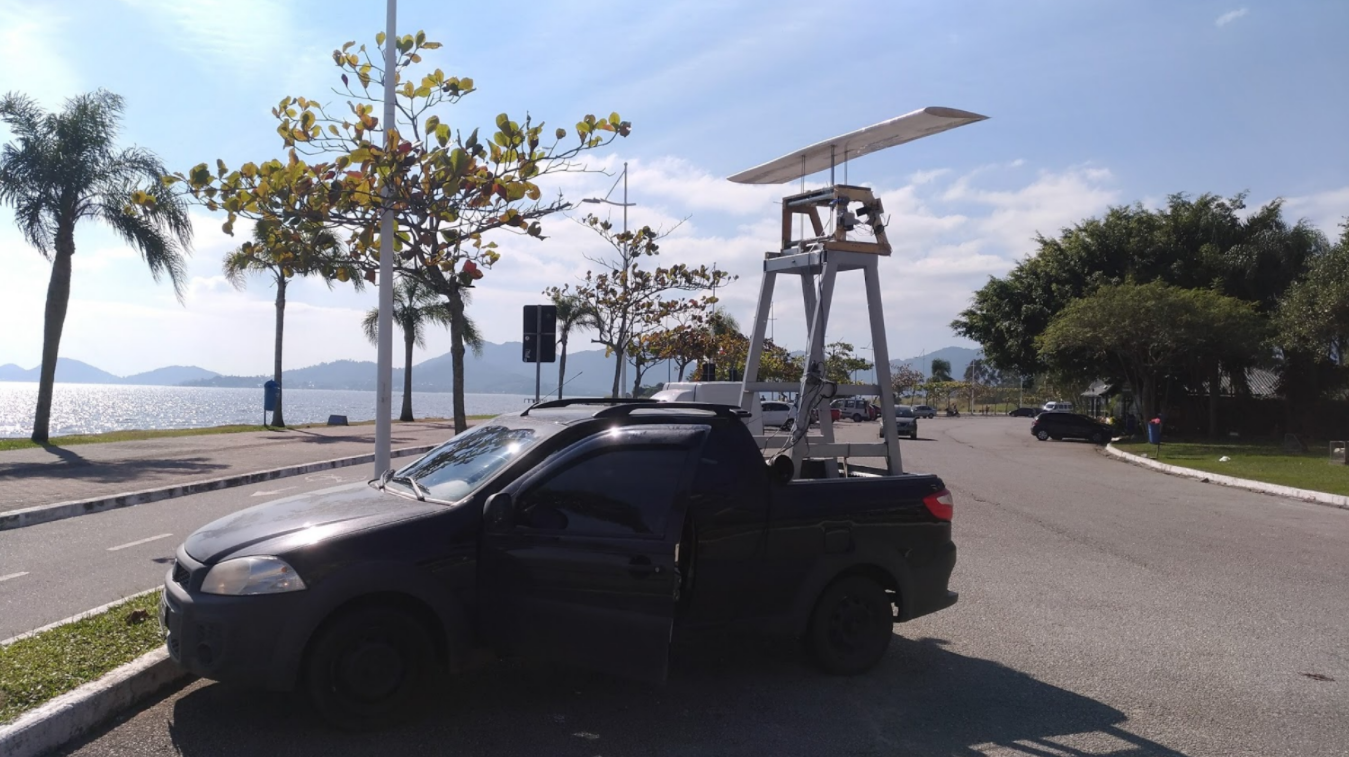
\includegraphics[width=0.4\columnwidth]{figuras/testes/bancada_mvp_1.png}}
        \label{fig:bancada11}
        \qquad
        \subfloat[]{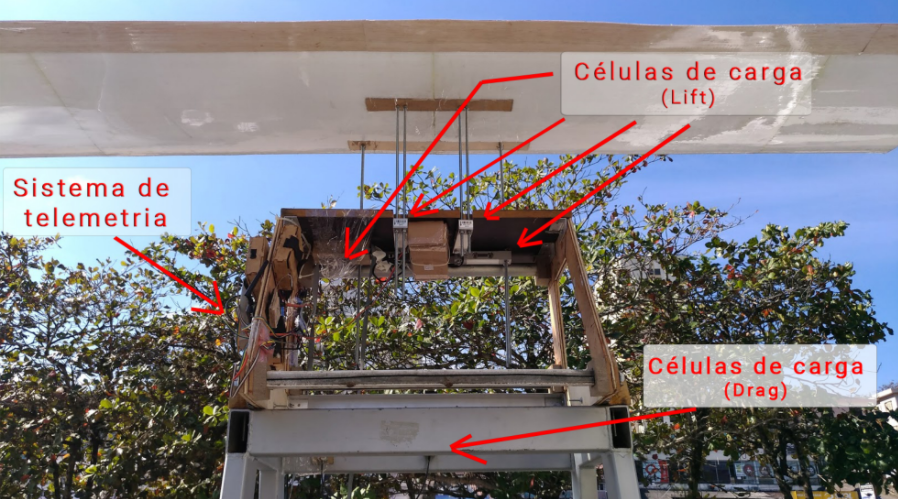
\includegraphics[width=0.4\columnwidth]{figuras/testes/bancada_mvp_2.png}}
        \label{fig:bancada12}
\end{figure}

Foi realizada uma serie de testes com esta bancada, entre eles o de medição de forças aerodinâmicas em uma asa, de medição do empuxo dinâmico em motor e de medição do momento causado pelo acionamento de superfícies de comando (ailerons) em uma asa. O procedimento destes testes e seus resultados esta detalhado em Lehmkuhl (2018). 

O MVP foi um sucesso no sentido de que provou o funcionamento da bancada proposta em curto espaço de tempo, porém possuía problemas estruturais intrínsecos as escolhas para a prototipagem mecânica, não demonstrando repetibilidade suficiente dos resultados. Além disso, ficaram claros diversos problemas do ponto de vista de execução, levantados por Lehmkuhl (2018), entre eles:

\begin{itemize}
    \item Aplicativo ainda em estágio inicial, apresentando uma interface pouco intuitiva
    \item Dificuldade para se ajustar o ângulo de incidência do dispositivo testado
    \item Problemas recorrentes de mal-contato elétrico, resultando na perda de baterias inteiras de dados
    \item Pouco controle sobre o estado e funcionamento do computador da bancada
    \item Configuração do teste no computador da bancada era realizado modificando-se o script original, o que tornava esta configuração bastante suscetível a erros pelo operador 
    \item Software embarcado (no computador da bancada) pouco organizado, com as estruturas de funcionamento do software altamente entrelaçadas, dificultando sua expansão e manutenção
    \item Falta de sincronia entre os dados das células de carga com relação aos outros sensores, o que tornava o processamento dos dados um processo bastante massante
    \item Falta de informações sobre o teste no arquivo de gravação dos dados, o que fazia com que o operador precisasse recorrer a outros meios para guardar a informação sobre o que e como estava sendo feito em cada bateria de testes, causando muitas vezes a perda de informação sobre as mesmas
    \item Falta de software para analise dos dados, o que tornava o processo de utilização dos dados gerados pela bancada uma tarefa altamente especializada
\end{itemize}

Estes pontos foram tomados como base para a segunda versão da bancada, detalhada neste texto e denominada "Bancada V1".

\section{Bancada V1}

Levando em conta os pontos levantados no MVP deu-se inicio a modelagem e construção da Bancada V1.

% \subsection{Modelo físico}

% COMENTAR SOBRE O MODELO ESTATICO E A CORRECAO DE FALSA SUSTENTACAO

\subsection{Mecânica}

A estrutura da bancada utilizando perfis extrudados em alumínio foi modelada no software Solidworks e é mostrada ja na figura \ref{fig:estrutura_bancada} para facilidade de entendimento das partes.

\begin{figure}[!ht]
    \centering
    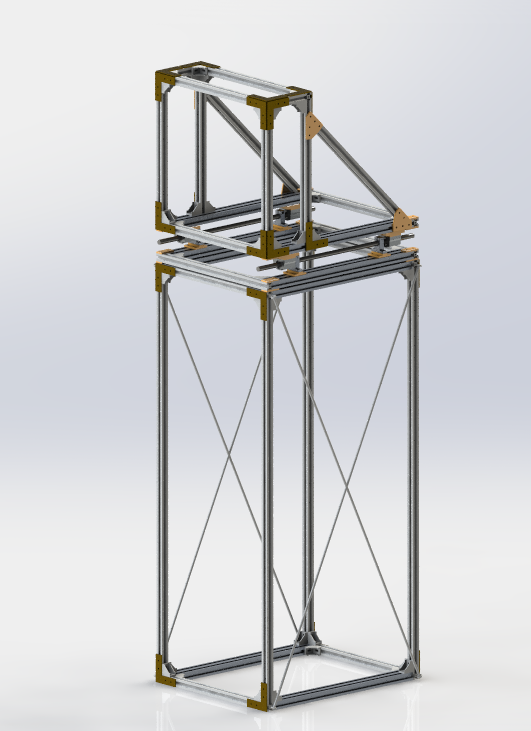
\includegraphics[width=.7\linewidth]{figuras/renders/estrutura_bancada_completa.png}
    \caption{Estrutura da bancada com conexões. Fonte: O autor.}
    \label{fig:estrutura_bancada}
\end{figure}

Os perfis de alumínio são adquiridos em barras de 1 metro de comprimento. A modelagem permitiu assim a definição das medidas dos cortes a serem realizados e a otimização do uso das barras.

% Para o projeto decidiu-se por evitar deslocamentos horizontais e verticais maiores que 1mm. Esta restrição visa limitar a 0.5 graus o ângulo maximo devido a deformaçao da balança em pitch em o acoplamento das mediçoes de sustenta que a deformação da bancada induza erros de alinhamento e consequentemente misture as medidas de sustentação e arrasto \cite{gonzalez2011components}.

As conexões estruturais foram feitas com cantoneiras planas de aço, garantindo rigidez nas juntas, agregando fidelidade na simulação (uma vez que nela as juntas são consideradas rígidas).

Para o encaixe das células de carga na bancada, assim como dos suportes das guias lineares e dos \textit{pillow-blocks}, foram projetados adaptadores que posteriormente foram produzidos via manufatura aditiva de polímero (figura \ref{adaptador_pillow}). Este método de manufatura permitiu a rápida prototipagem dessas peças e acelerou o desenvolvimento do projeto.

\begin{figure}[!ht]
    \centering
    \caption{Adaptadores impressos para as células de carga. Fonte: O autor.}
        \subfloat[Adaptadores para encaixe das células de carga de sustentação e momento.]{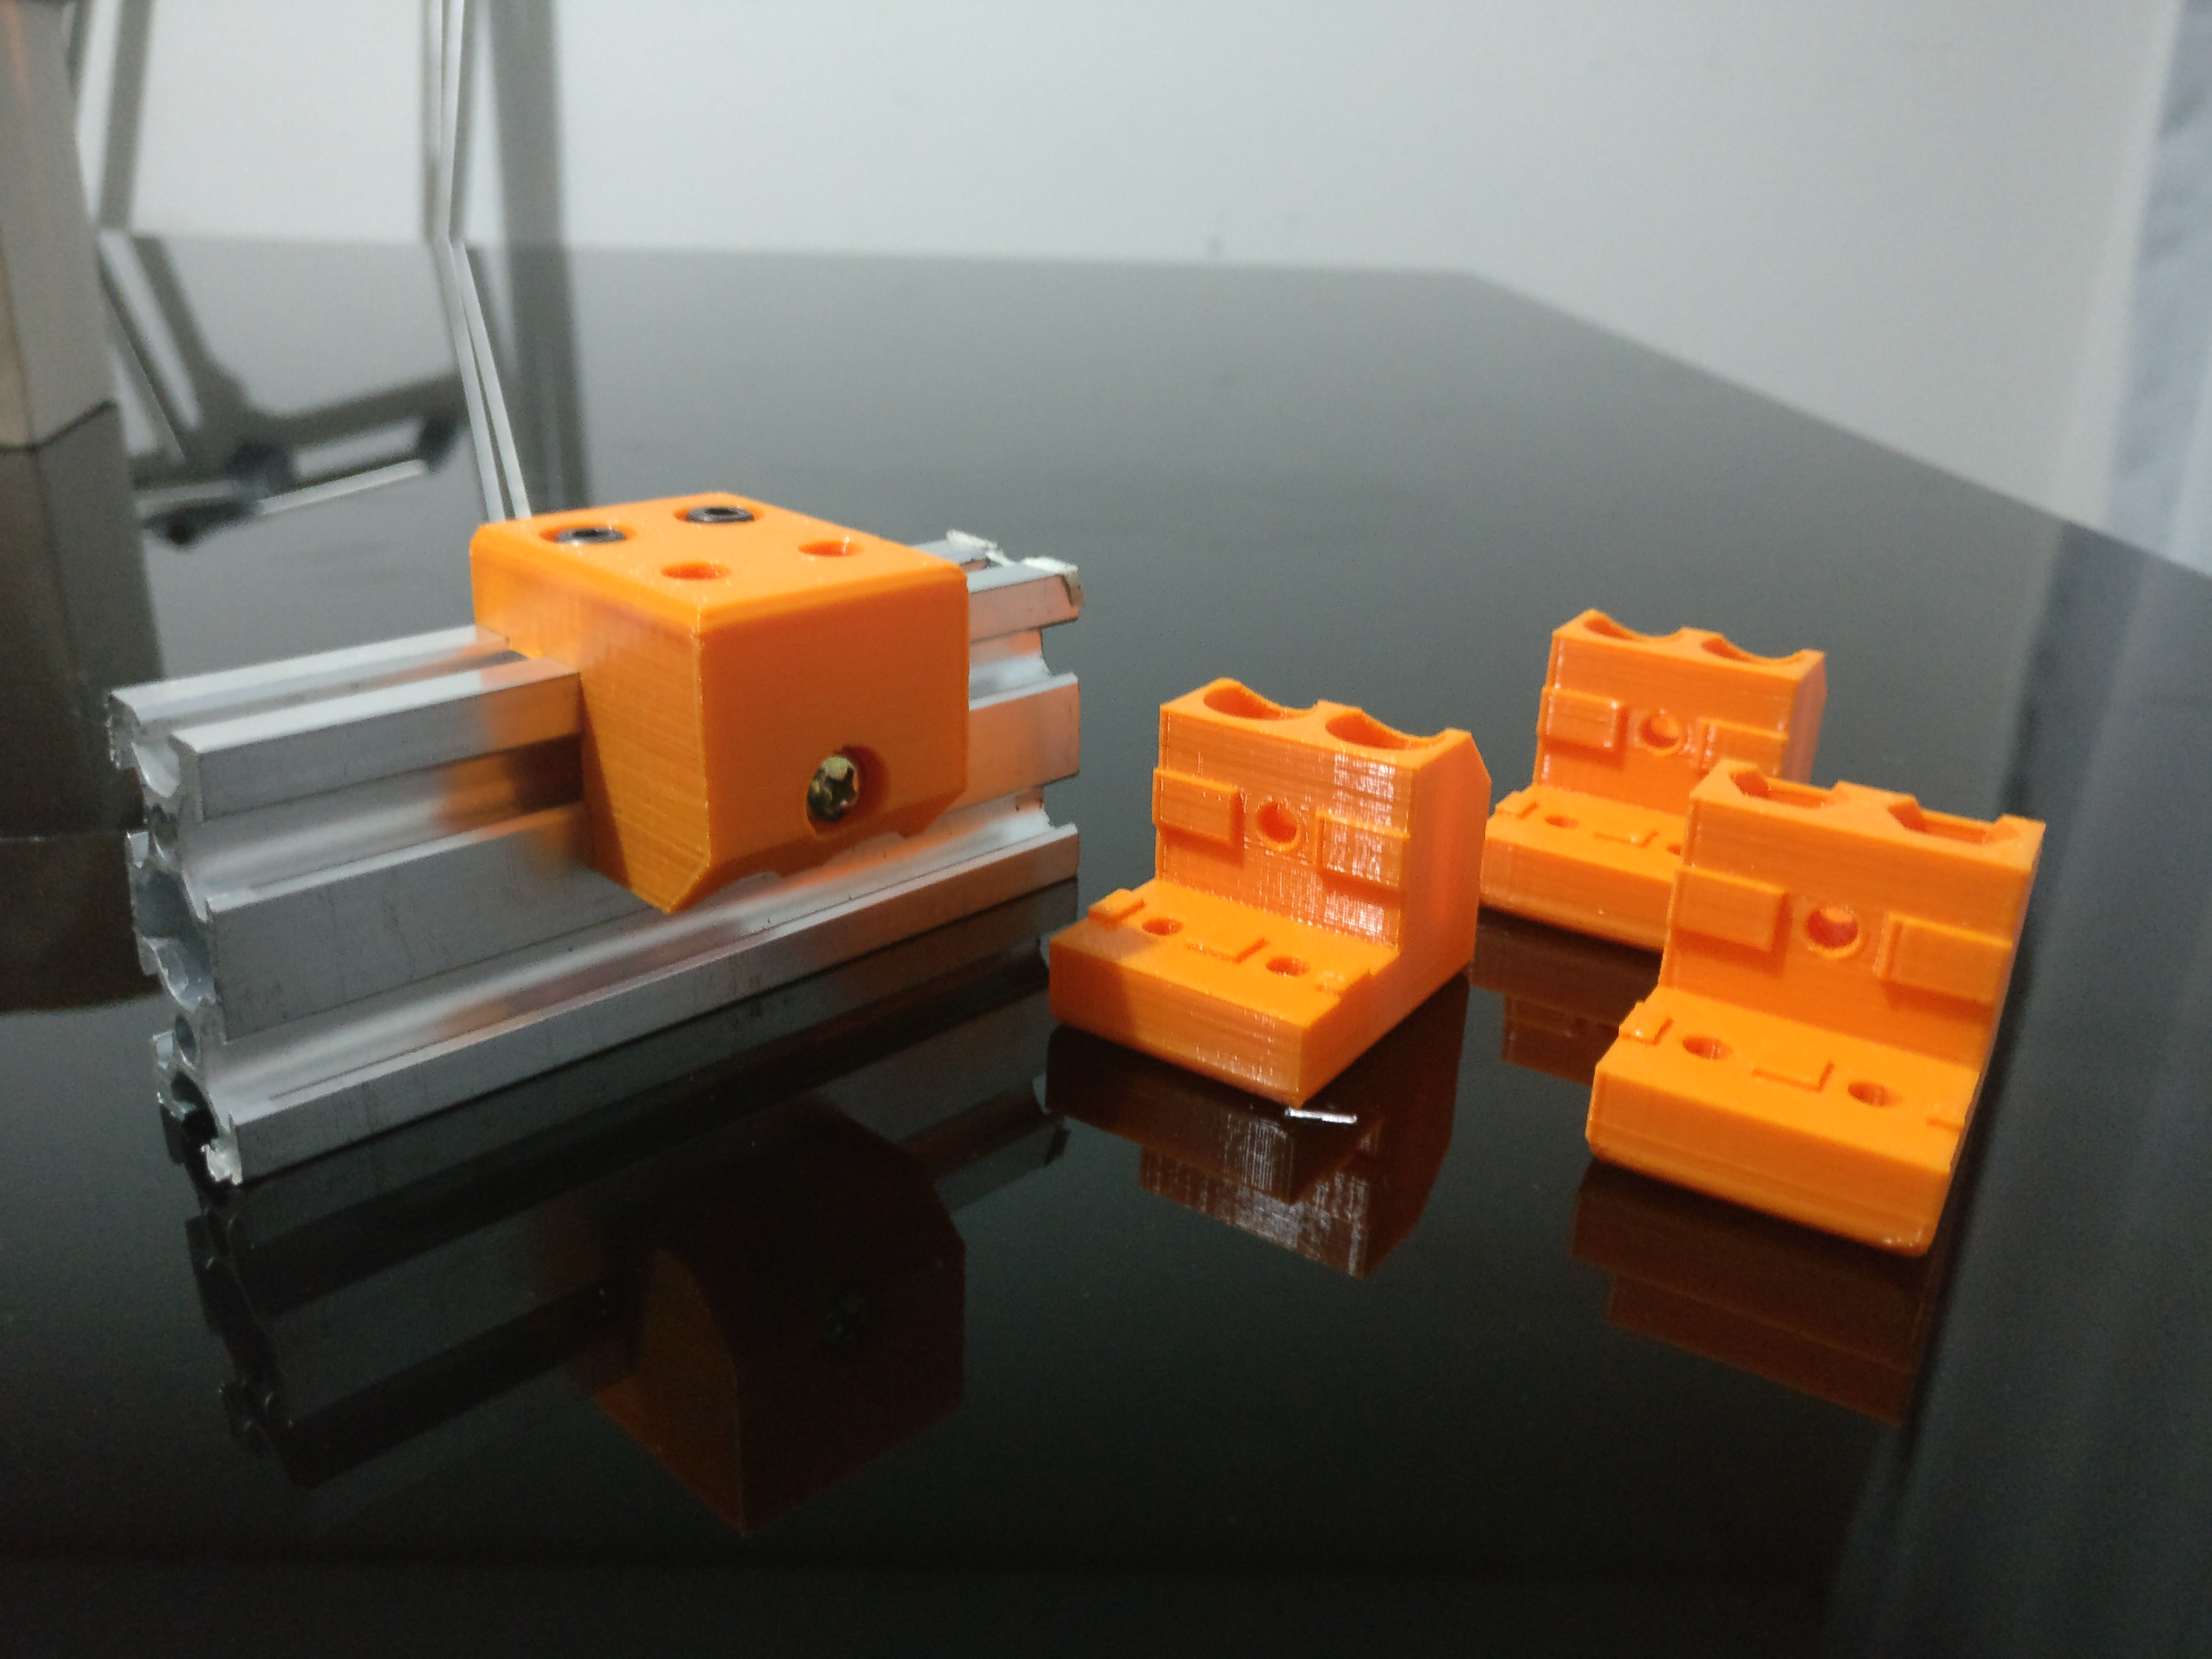
\includegraphics[width=0.4\columnwidth]{figuras/construcao/suporte_reforcado_celulas_3.jpg}}
        \label{encaixe_celulas_sustentacao}
        \qquad
        \subfloat[Células de carga de sustentação e momento com adaptador.]{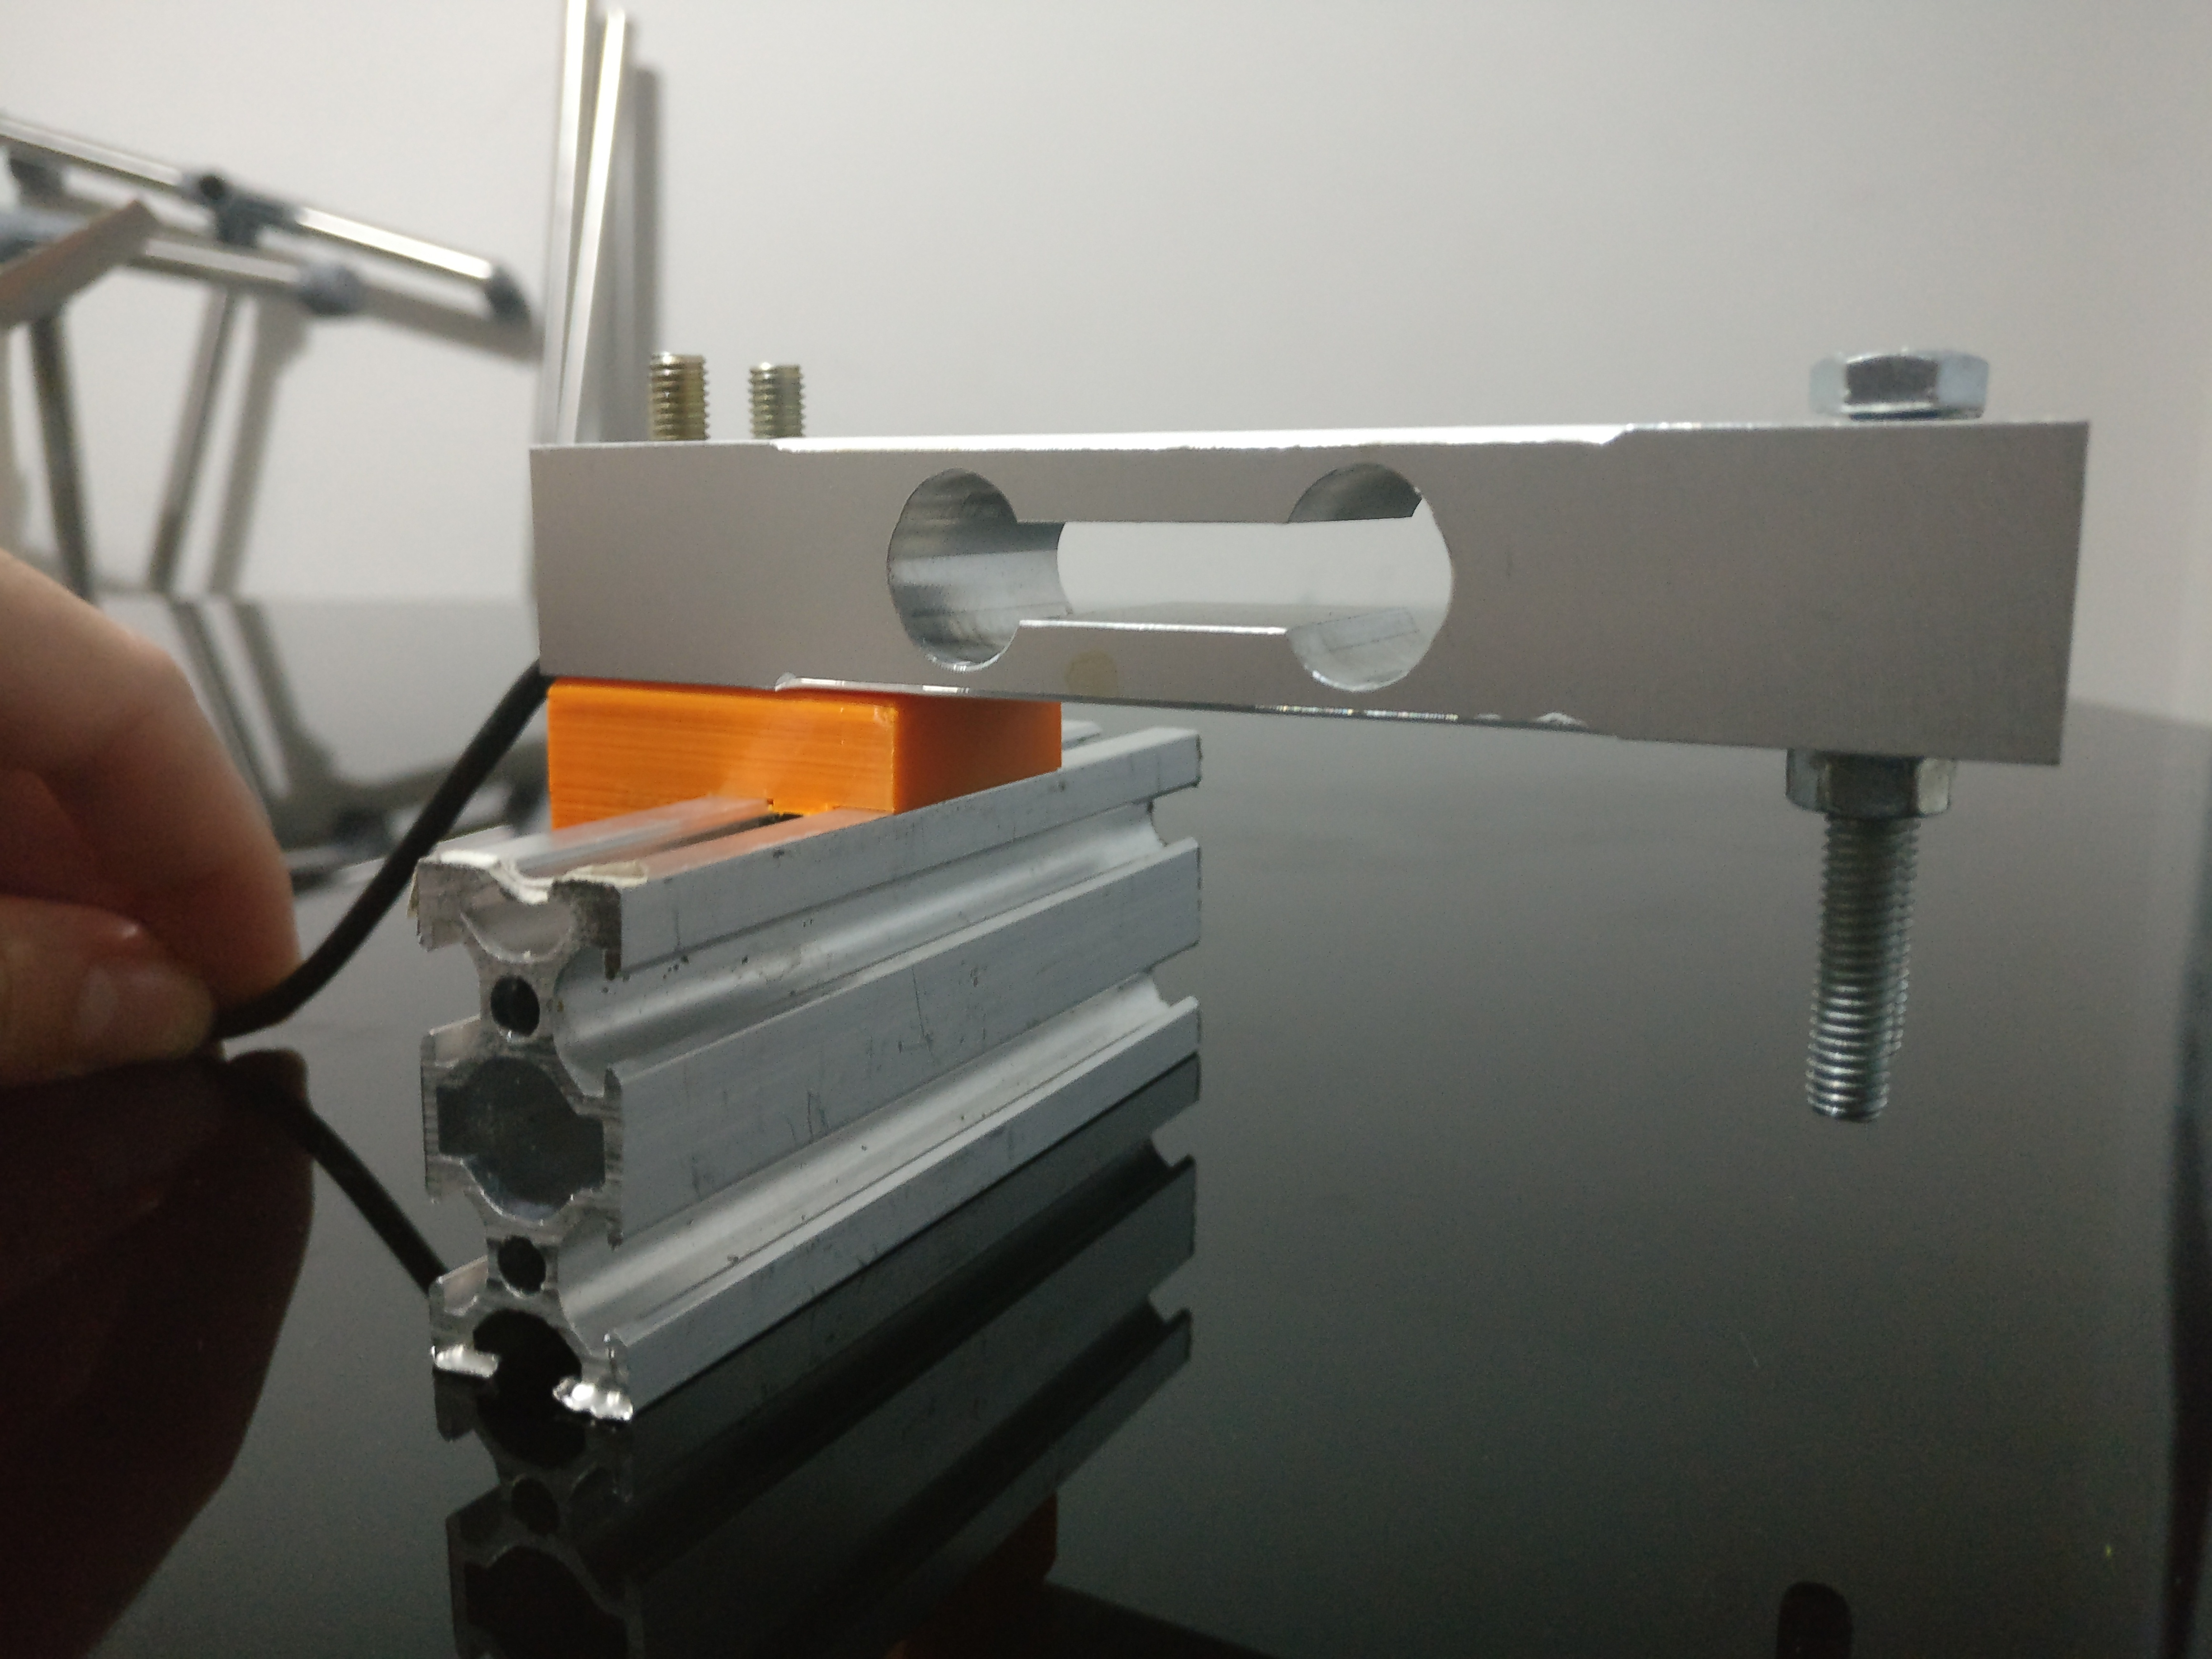
\includegraphics[width=0.4\columnwidth]{figuras/construcao/suporte_reforcado_celulas_1.jpg}}
        \label{encaixe_celulas_sustentacao_2}
\end{figure}

\begin{figure}[!ht]
    \centering
    \caption{Adaptadores para Pillow-Block e Suporte SK12. Fonte: O autor.}
        \subfloat[Adaptador para encaixe do Pillow Block ("carrinho") na bancada.]{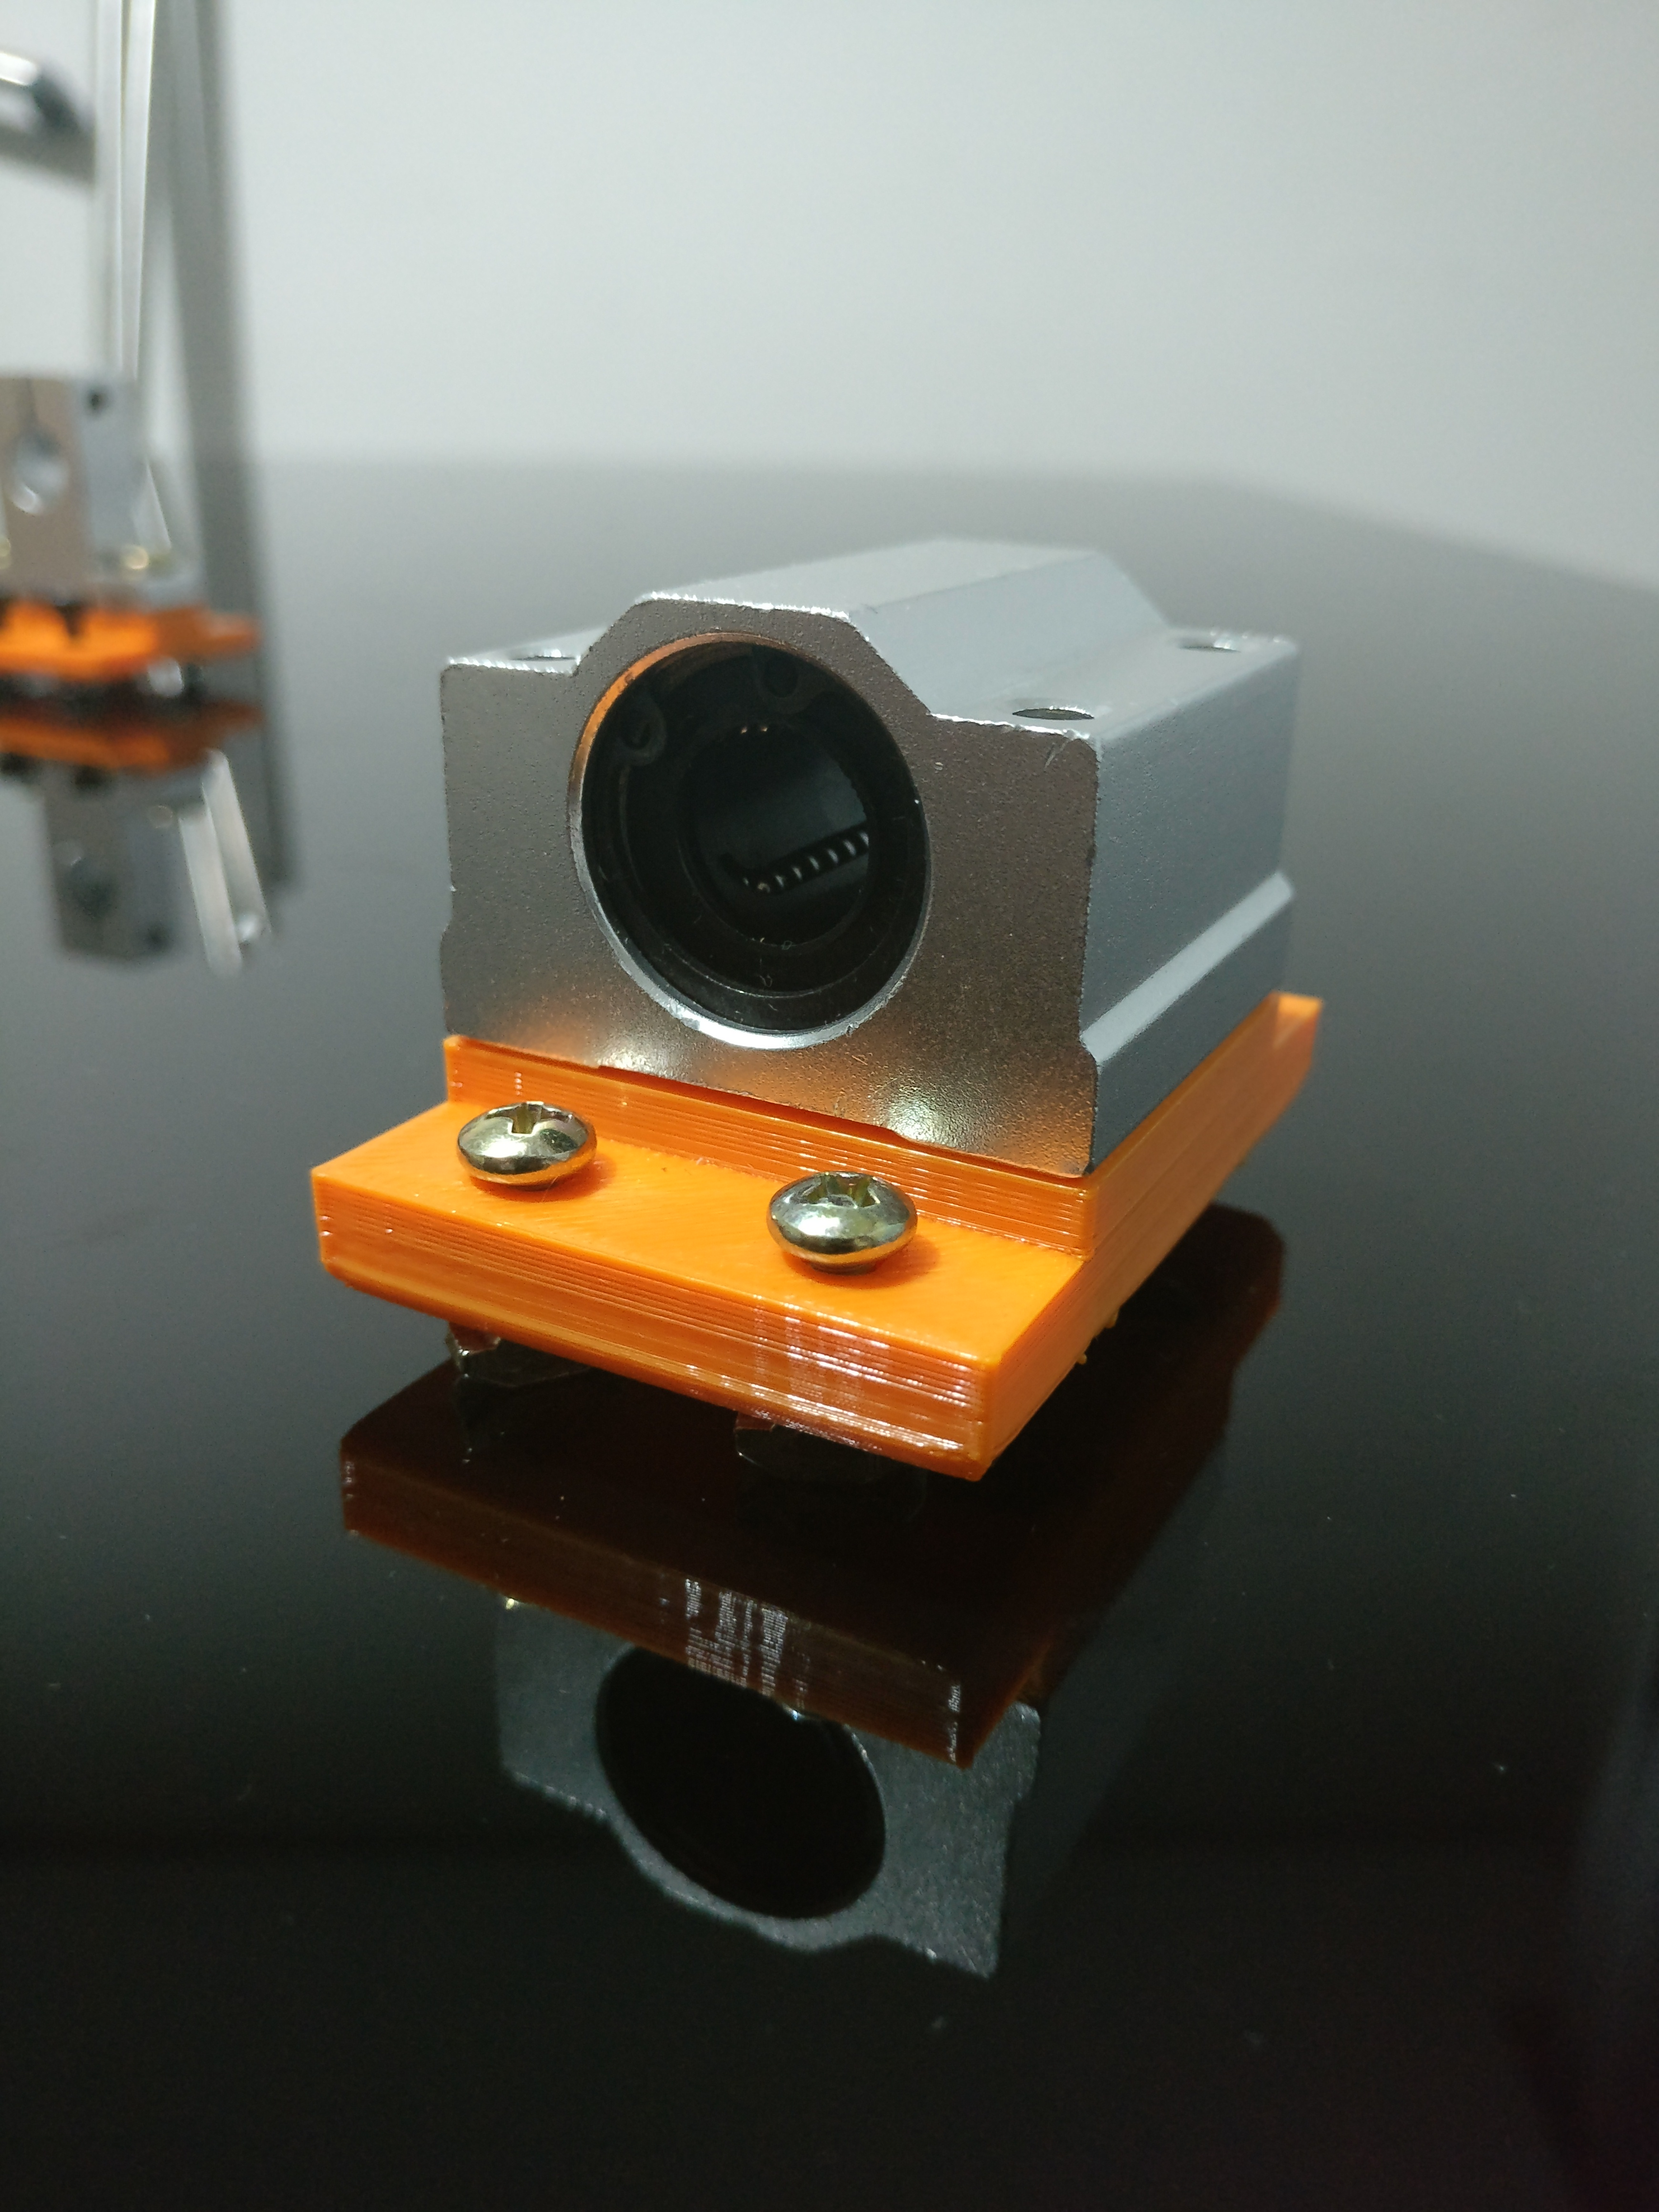
\includegraphics[width=0.4\columnwidth]{figuras/construcao/encaixe_pillow.jpg}}
        \label{adaptador_pillow}
        \qquad
        \subfloat[Adaptador para encaixe dos suportes das guias lineares na bancada.]{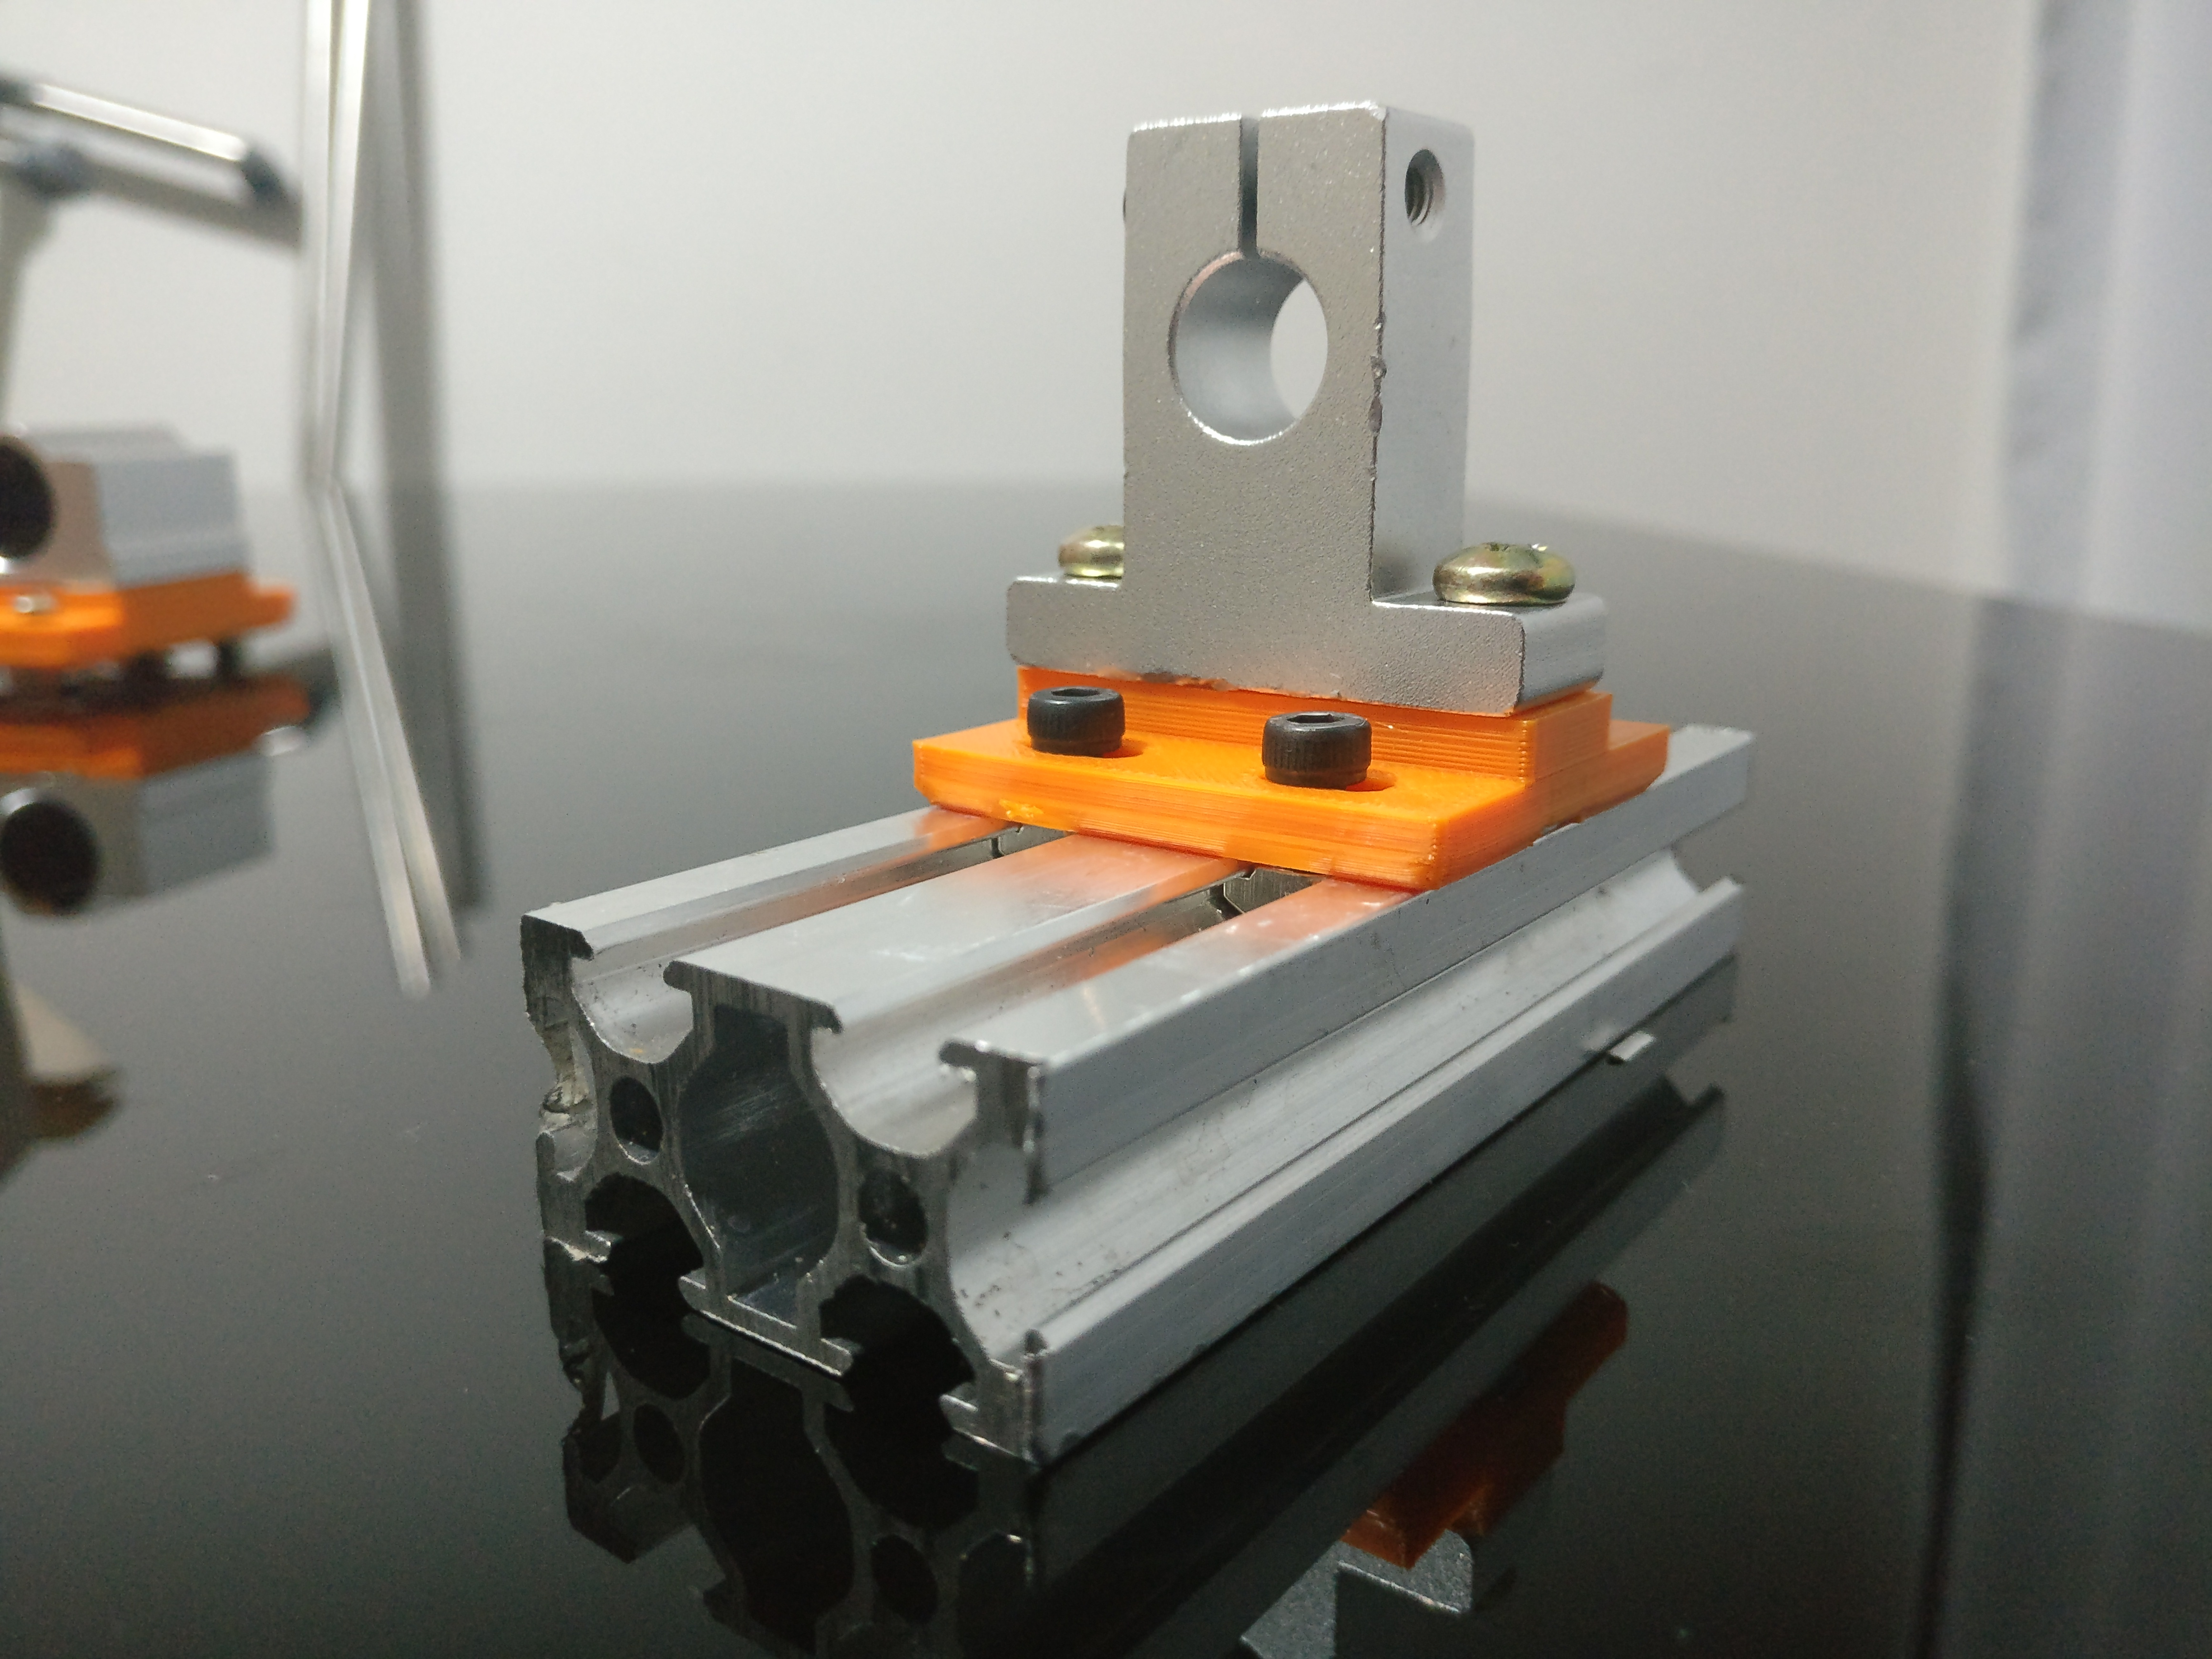
\includegraphics[width=0.4\columnwidth]{figuras/construcao/encaixe_sk12.jpg}}
        \label{adaptador_sk12}
\end{figure}

Devido à dificuldade na simulação de peças produzidas por este processo, que possuem alta anisotropia e grande dispersão nos resultados dependendo da qualidade da impressão \citep{montero2001material}, foram realizados testes estruturais estáticos para se garantir que as peças não falhassem.

Cabe aqui um adendo de que, para se garantir ainda maior rigidez à bancada como um todo, é de interesse a produção dessas peças em metal, realizando as devidas modificações para melhor se adequar ao processo de manufatura escolhido. A produção dessas peças em metal contudo não foi realizada dentro do tempo do presento trabalho.

Dado que a bancada não teve seu movimento em X restrito exclusivamente por células de carga (como foi o caso no eixo Z), foi necessário permitir liberdade de movimento neste sentido, de modo que o carregamento se desse quase que exclusivamente na célula de carga. Para isto foram instaladas guias lineares nesta direção (figura \ref{guias_lineares}). Esta solução possui baixo atrito, além de apresentar pouquíssima folga no sentido transversal ao eixo da guia, o que favorece o alinhamento da bancada.

Como as guias possuem pouca folga, a tolerância de montagem também é pequena, isto é, uma pequena angulação entre os dois trilhos causaria travamento do sistema, o que é indesejado. Para permitir ajuste desse ângulo durante a montagem das mesmas foi modelado um rasgo nas peças de encaixe dos trilhos, como mostrado na figura \ref{rasgo_suporte_sk12}. Assim pode-se correr as guias durante a instalação e ajustar o ângulo de modo a garantir o não travamento.

\begin{figure}[!ht]
    \centering
    \caption{Soluções desenvolvidas para a estrutura da bancada. Fonte: O autor.}
        \subfloat[Detalhe do rasgo permitindo flexibilidade na instalação das guias.]{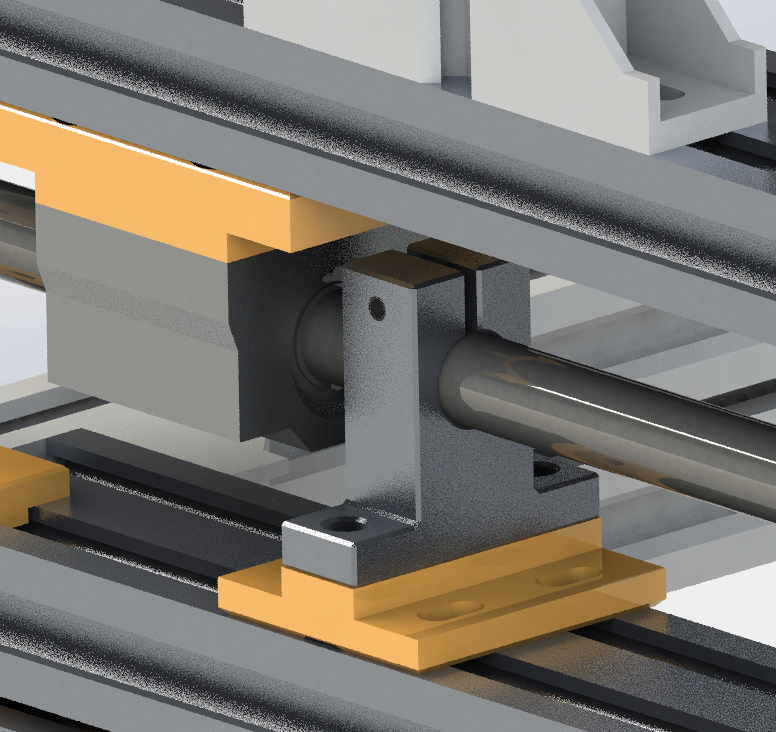
\includegraphics[width=0.4\columnwidth]{figuras/renders/suporte_sk12_com_rasgo.png}}
        \label{rasgo_suporte_sk12}
        \qquad
        \subfloat[Solução de guias lineares construída.]{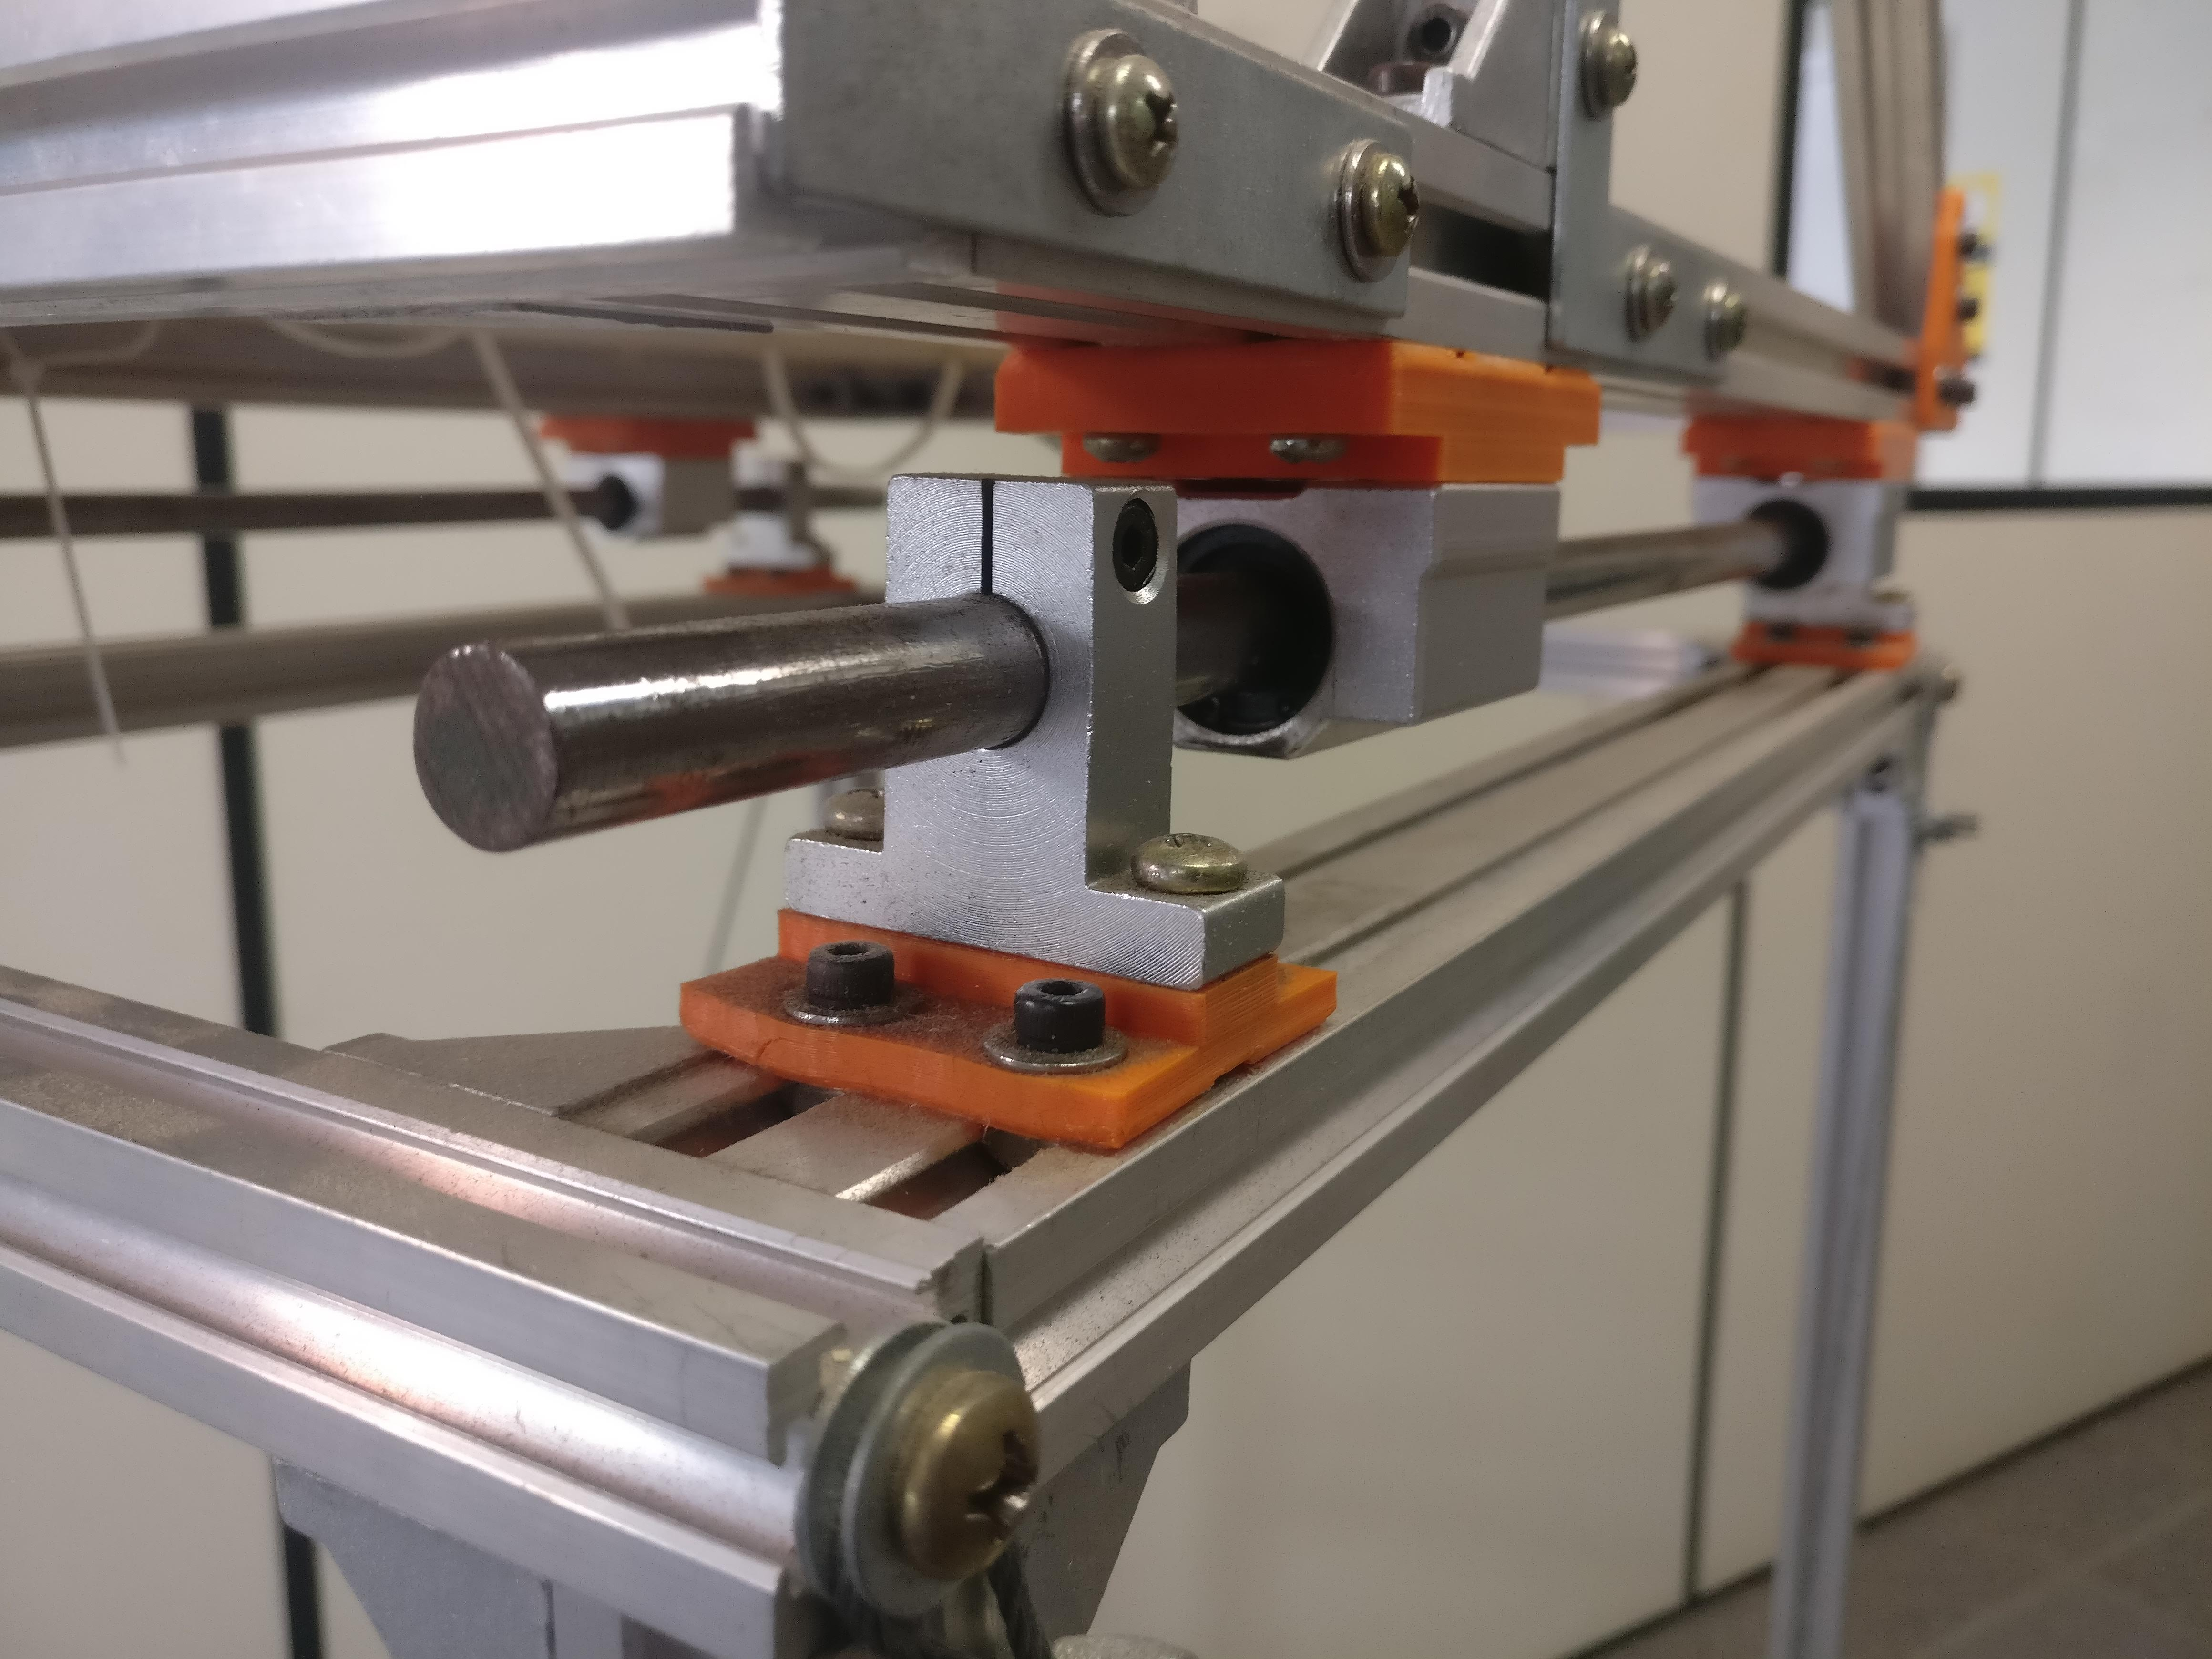
\includegraphics[width=0.4\columnwidth]{figuras/calibracao/guias_lineares.jpg}}
        \label{guias_lineares}
\end{figure}

\begin{figure}[!ht]
    \centering
    \caption{Soluções desenvolvidas para a estrutura da bancada. Fonte: O autor.}
        \subfloat[Reforço estrutural com cabos de aço.]{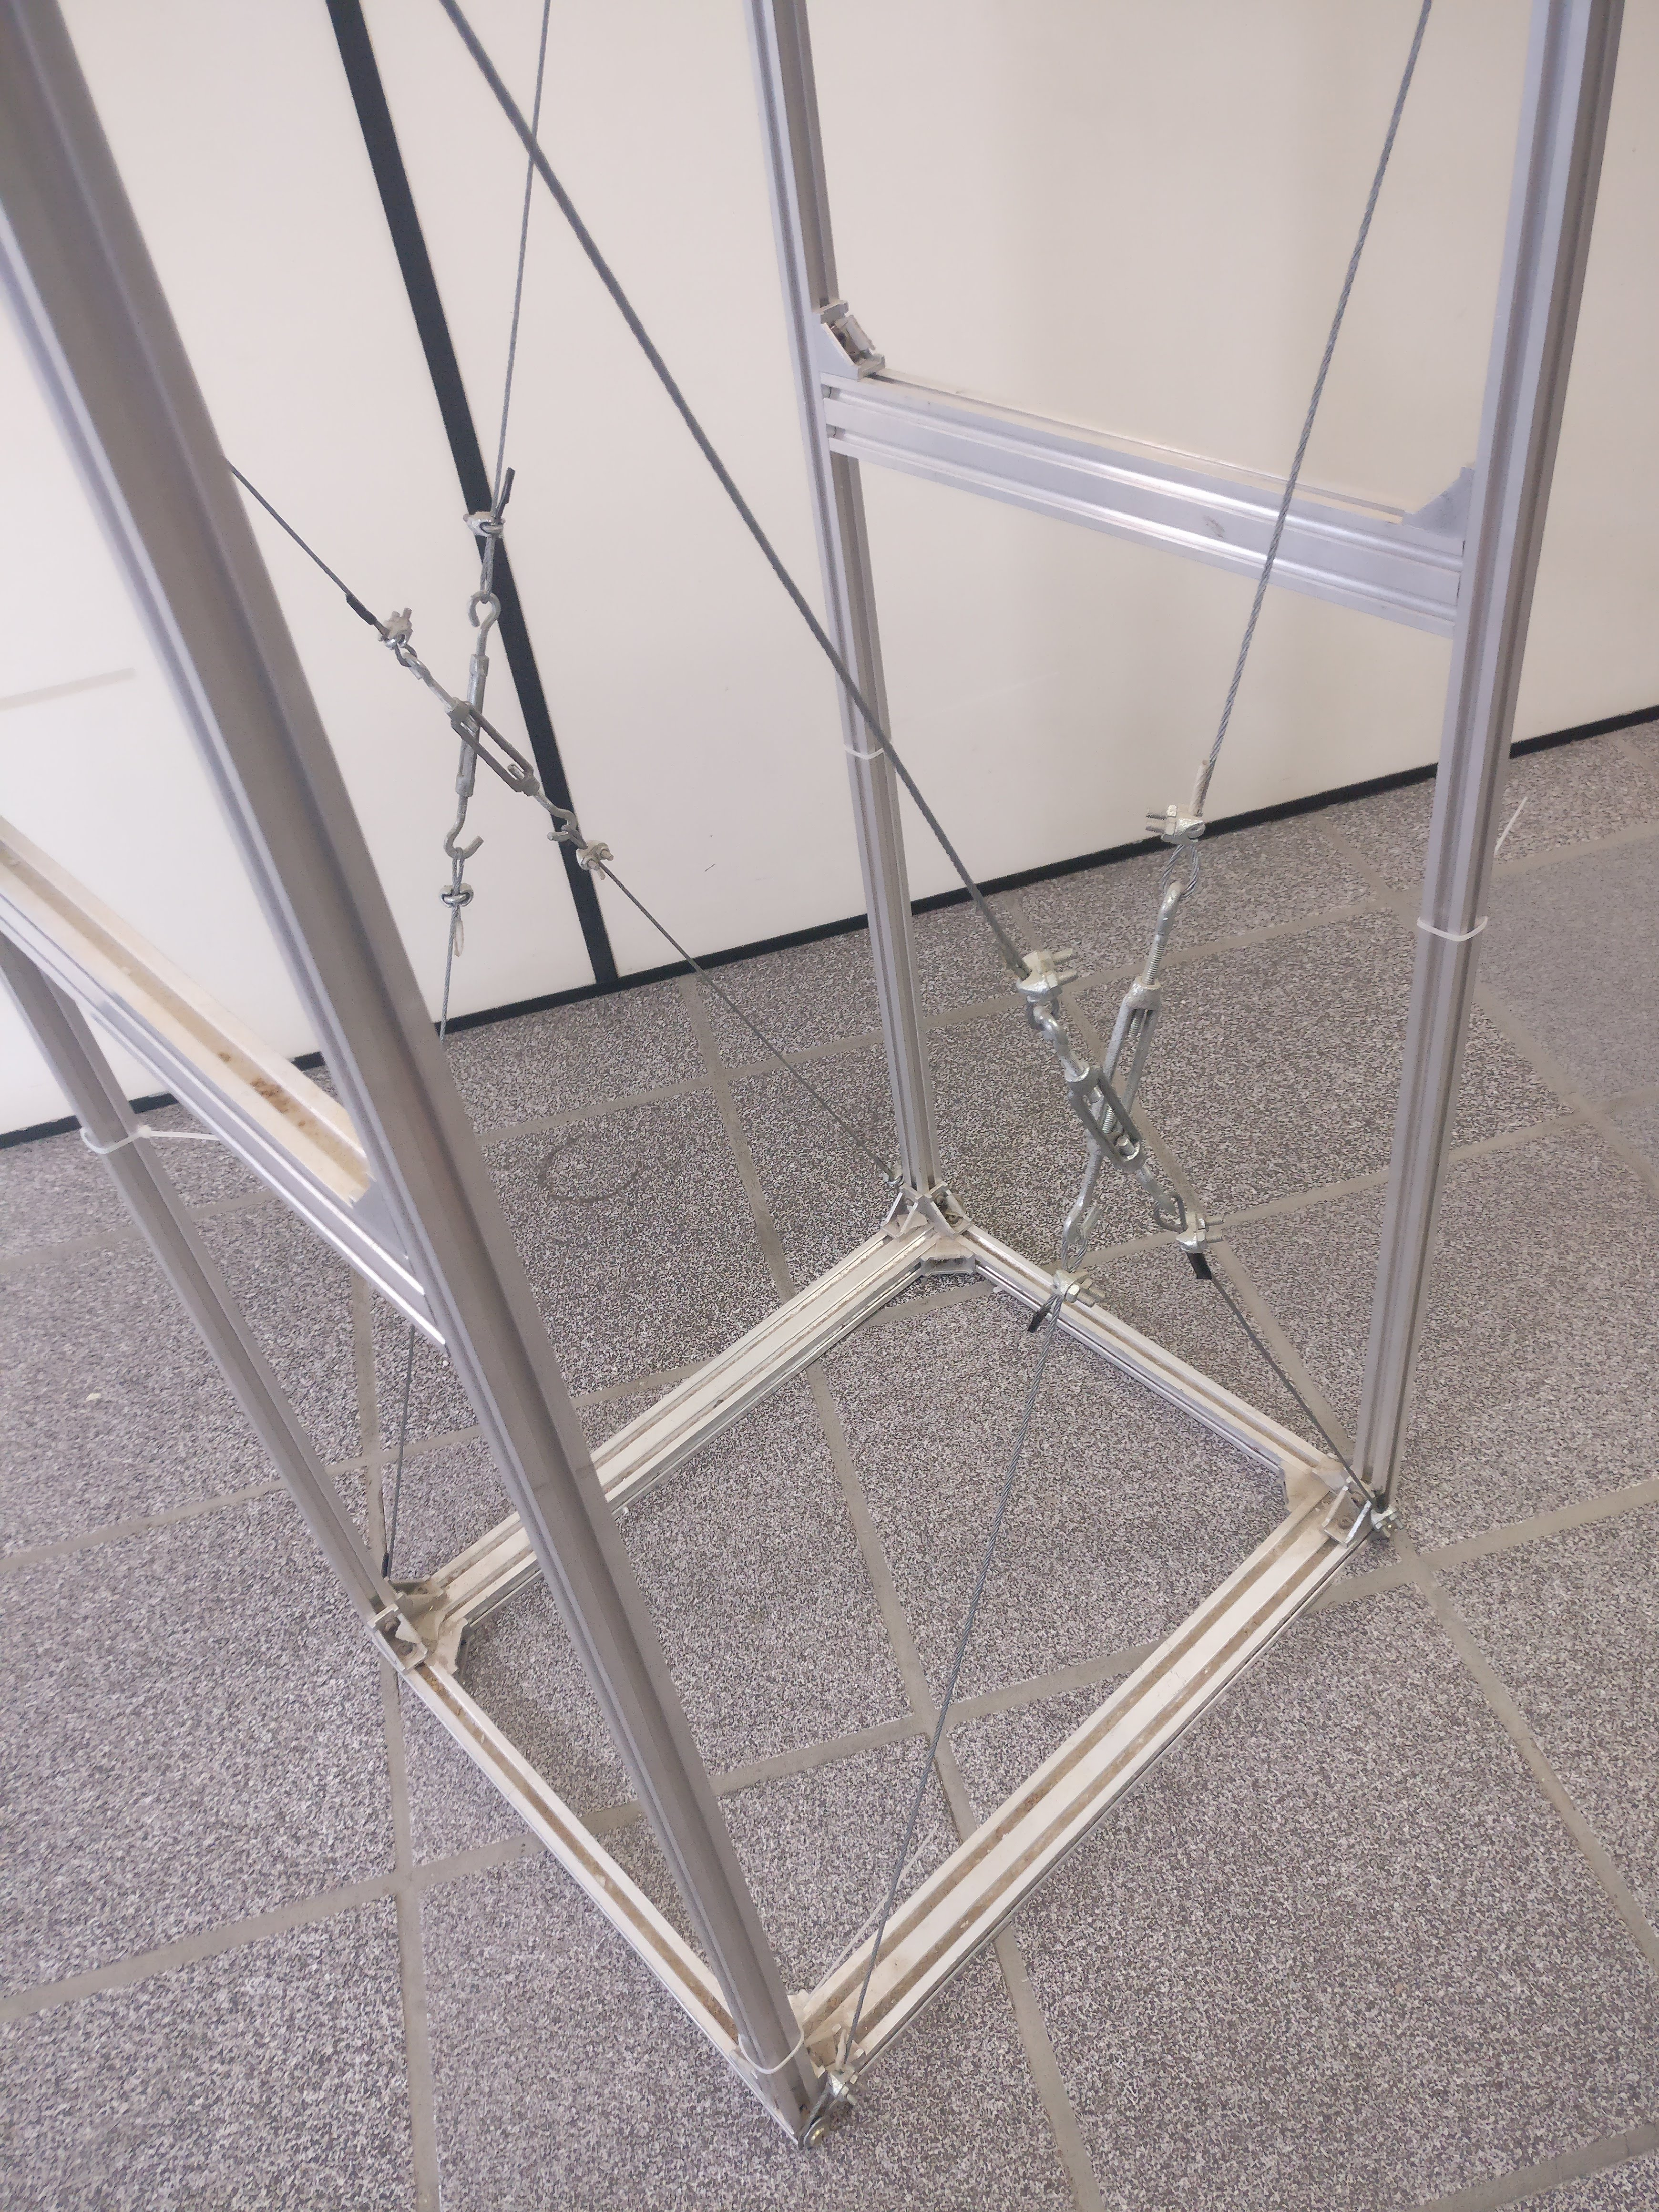
\includegraphics[width=0.4\columnwidth]{figuras/calibracao/reforco_cabos_aco.jpg}}
        \label{cabos_aco}
        \qquad
        \subfloat[Reforço estrutural utilizado nas conexões da bancada.]{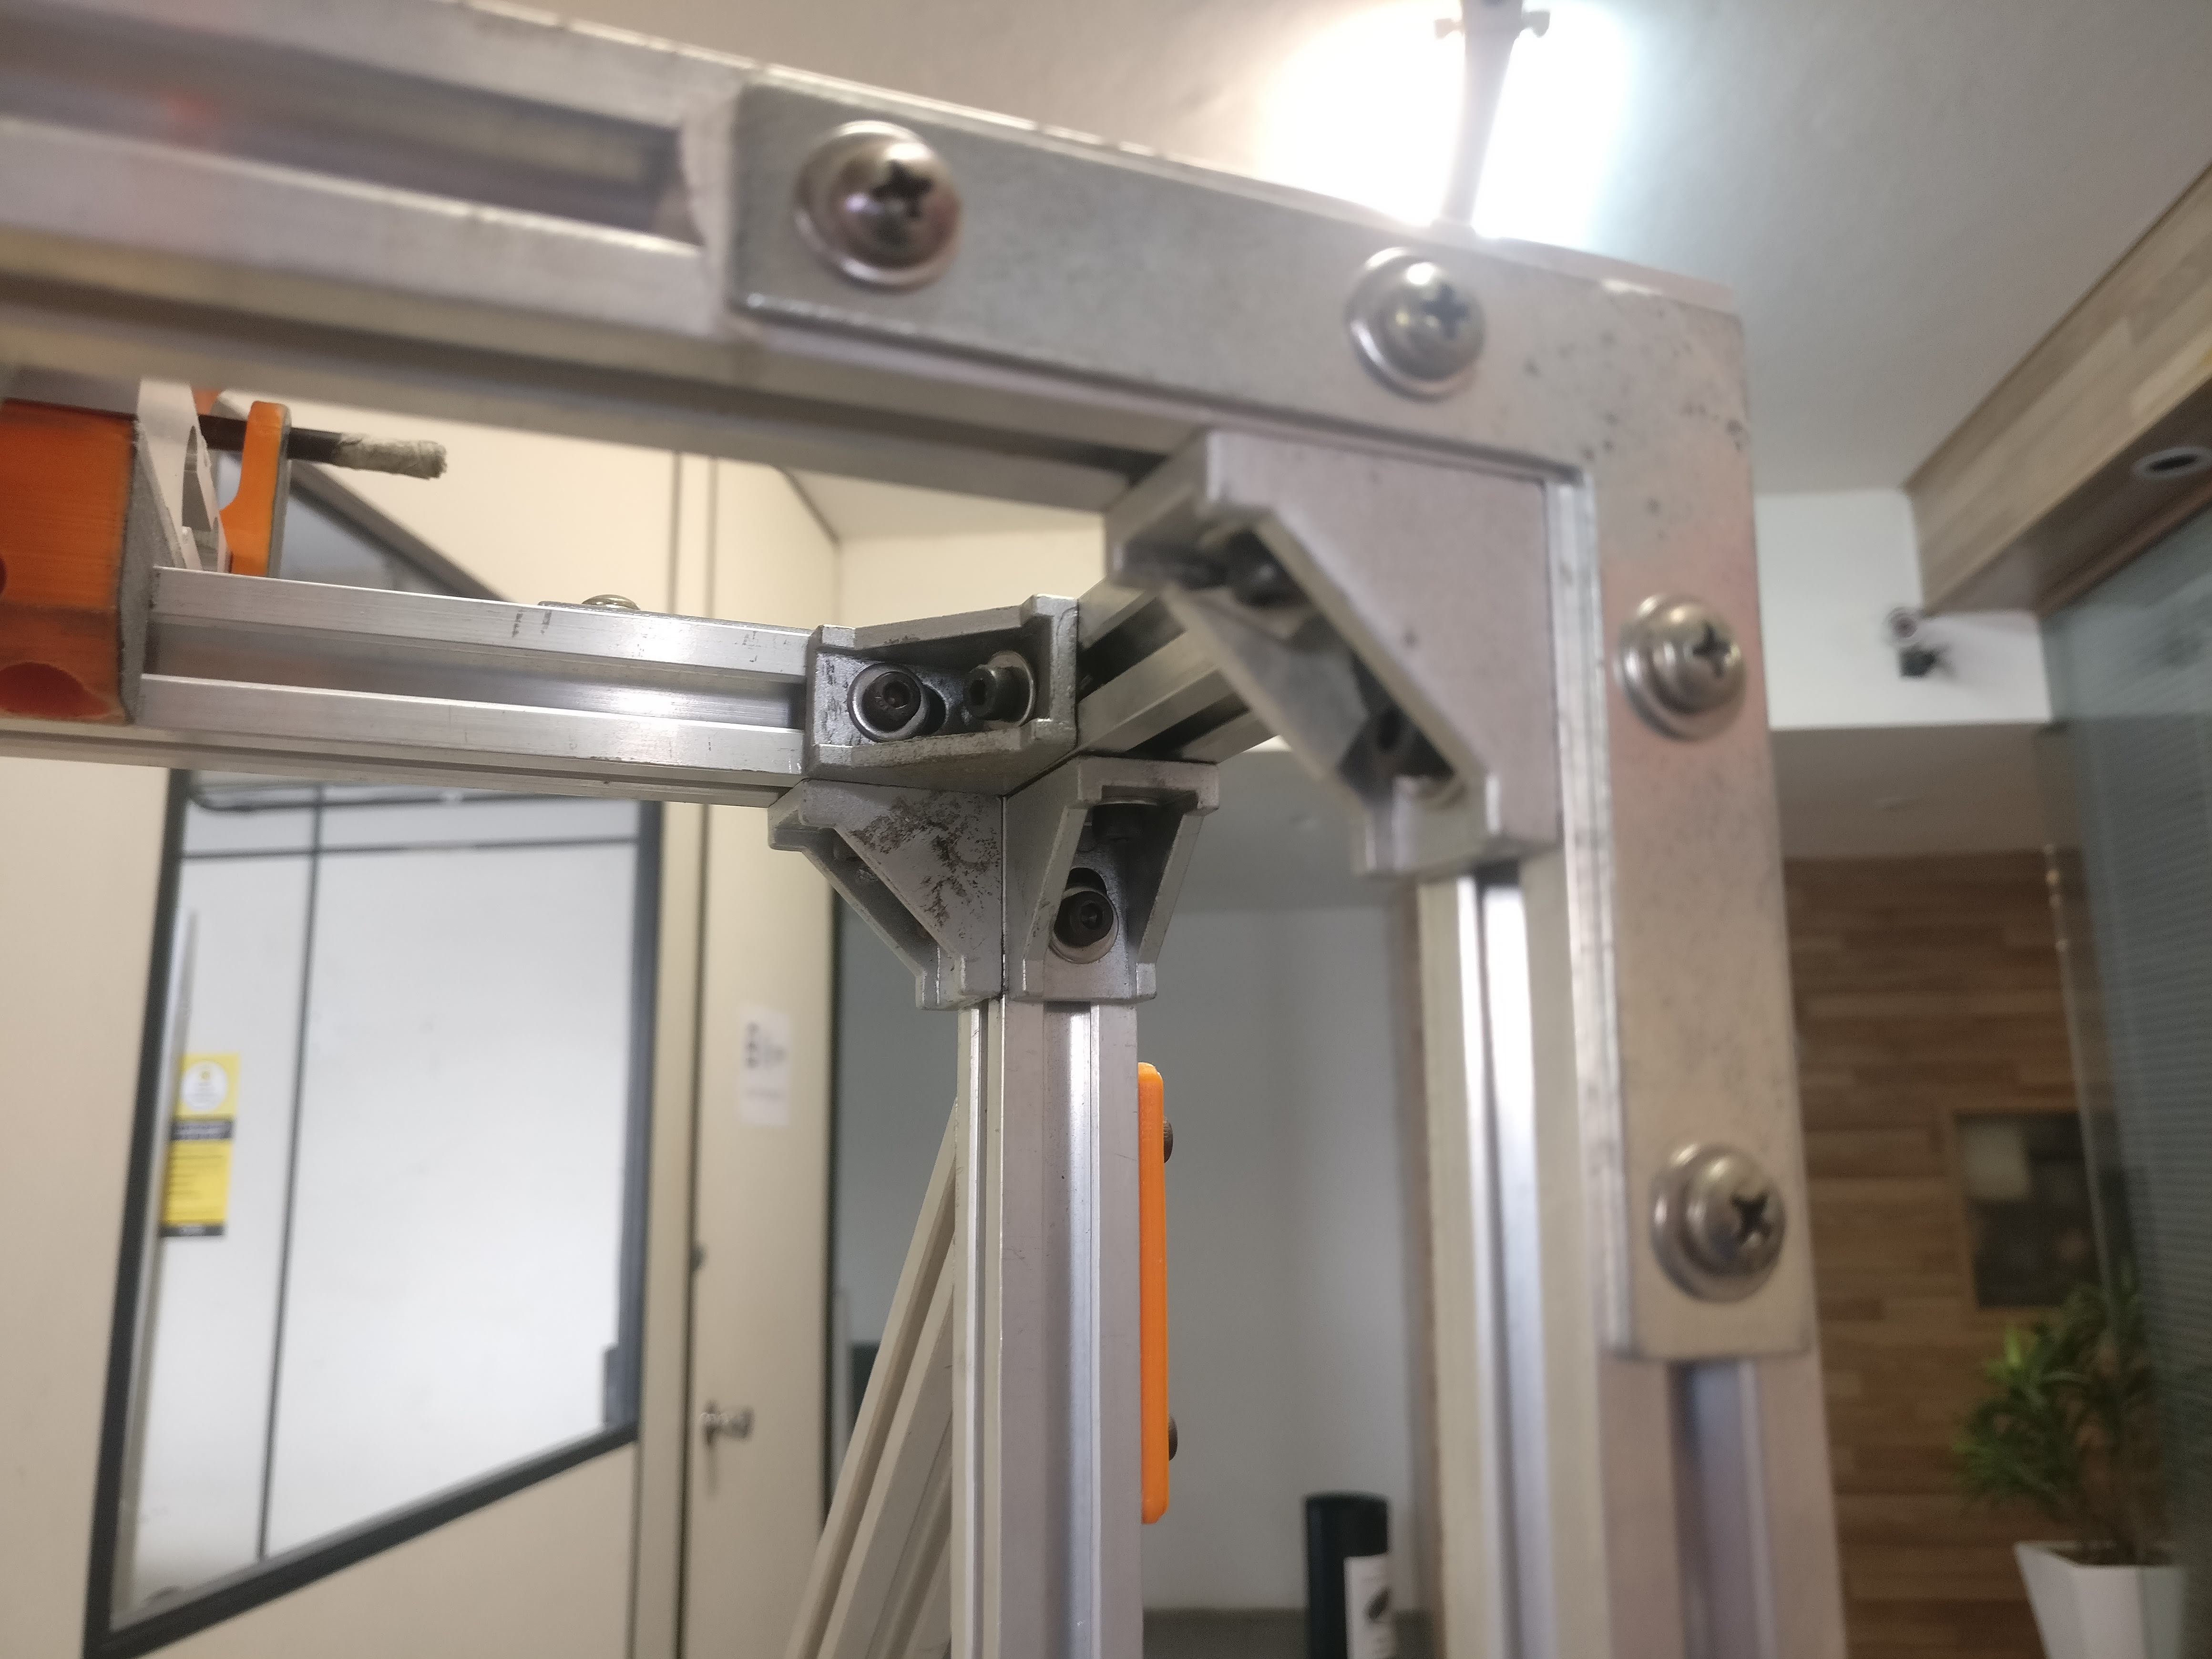
\includegraphics[width=0.4\columnwidth]{figuras/calibracao/reforco1.jpg}}
        \label{reforco_estrutural}
\end{figure}

A solução ideal para se garantir rigidez torcional da torre ao longo do eixo Z seria o treliçamento das laterais com os perfis de alumínio. Esta solução porem elevaria o custo do projeto para além do que a equipe possuía de verba disponível. A solução encontrada foi treliçar as duas laterais com cabos de aço (figura \ref{cabos_aco}).

Os furos dos quatro cantos da bancada foram rosqueados e argolas de fixação e cabos de aço foram instalados nas duas laterais, com tensionadores de modo a facilitar a instalação mesmo com pequenos desvios no comprimento dos cabos.

A primeira bancada utilizava barras roscadas como solução para o ajuste de ângulo de incidência do componente testado. Esta solução possuía três problemas principais:

\begin{itemize}
    \item Ajuste demorado, pois era necessário girar as duas barras até o ângulo desejado medindo este ângulo com o auxilio de um nível digital.
    \item Dificuldade no alinhamento da altura das duas barras, o que causava uma inclinação lateral no componente.
    \item Pouca precisão no ajuste do ângulo.
\end{itemize}

A solução encontrada foi trocar o ajuste continuo por um ajuste discreto, utilizando furos com angulação previamente projetada, como mostrado nas figuras \ref{peca_ângulo_0}a e \ref{peca_ângulo_18}b.

\begin{figure}[!ht]
    \centering
    \caption{Detalhe da peça de ajuste discreto de ângulo de incidência. Fonte: O autor.}
        \subfloat[Ajuste a 0 graus.]{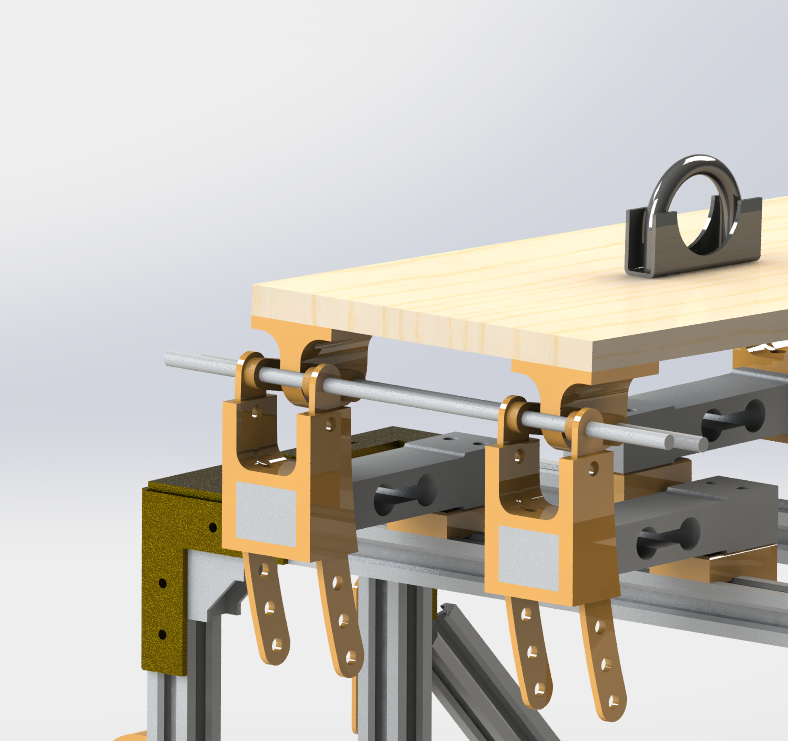
\includegraphics[width=0.4\columnwidth]{figuras/renders/detalhe_ajuste_angulo_0_graus.png}}
        \label{peca_ângulo_0}
        \qquad
        \subfloat[Ajuste a 18 graus.]{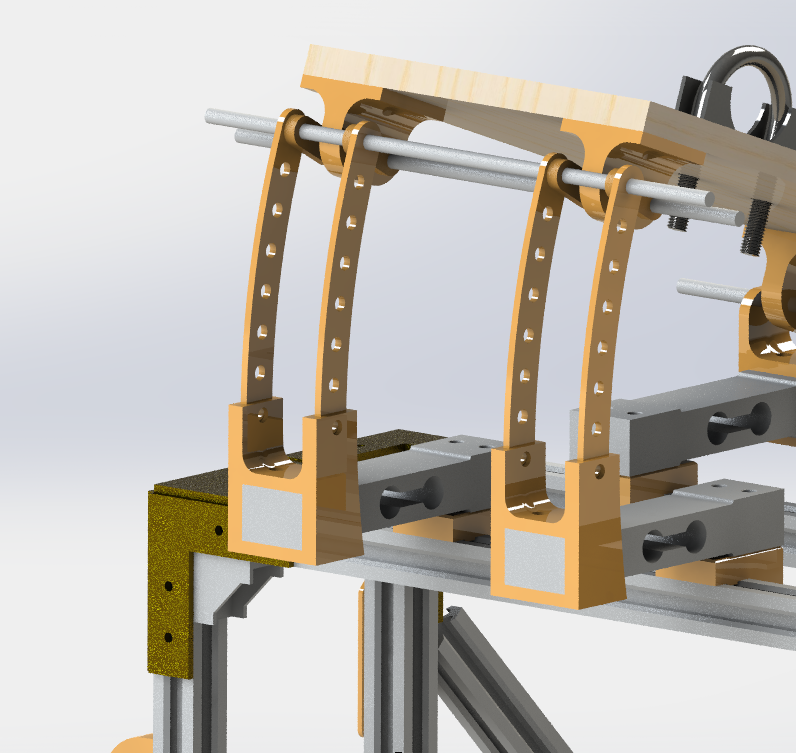
\includegraphics[width=0.4\columnwidth]{figuras/renders/detalhe_ajuste_angulo_18_graus.png}}
        \label{peca_ângulo_18}
\end{figure}

Esta solução garante que os mesmos ângulos sempre serão utilizados nos testes, o que adiciona facilidade no processamento posterior dos dados.

Os ângulos escolhidos foram: 0, 3, 6, 9, 12, 15 e 18 graus.

O principal problema desta solução é não permitir ajustes finos no ângulo, o que a principio será um problema apenas caso se deseje descobrir o ângulo de estol de asas. Este problema porem é tido como pequeno frente aos enfrentados com a solução anterior, e pode ser contornado fabricando-se uma peça de ajuste com mais furações e/ou uma peça de ajuste continuo a ser usada especificamente no teste de estol.
\subsection{Eletronica}

Como um dos maiores problemas do MVP foi o de falha no sistema eletrônico devido a mal-contato, atenção especial foi dada a esta parte. Duas soluções foram propostas:

\begin{itemize}
    \item Produção de placas de circuito impresso para todos os sistemas
    \item Utilização de conectores mais robustos
\end{itemize}

Foram projetadas e produzidas duas PCBs: uma para os transdutores de célula de carga e outra para os transdutores de pressão diferencial.

\begin{figure}[!ht]
    \centering
    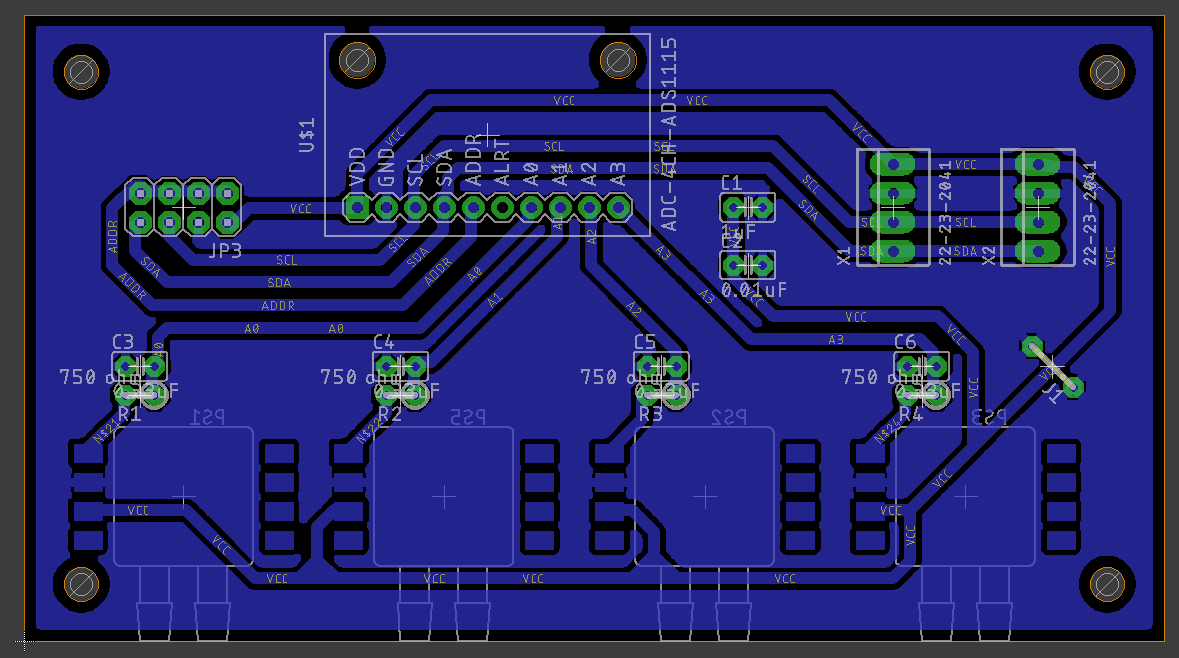
\includegraphics[width=.8\linewidth]{figuras/renders/pitot_board.png}
    \caption{Projeto da placa de transdutores de pressão diferencial no software Eagle\cite{autor}.}
    \label{fig:projeto_pcb_pitot}
\end{figure}

\begin{figure}[!ht]
    \centering
    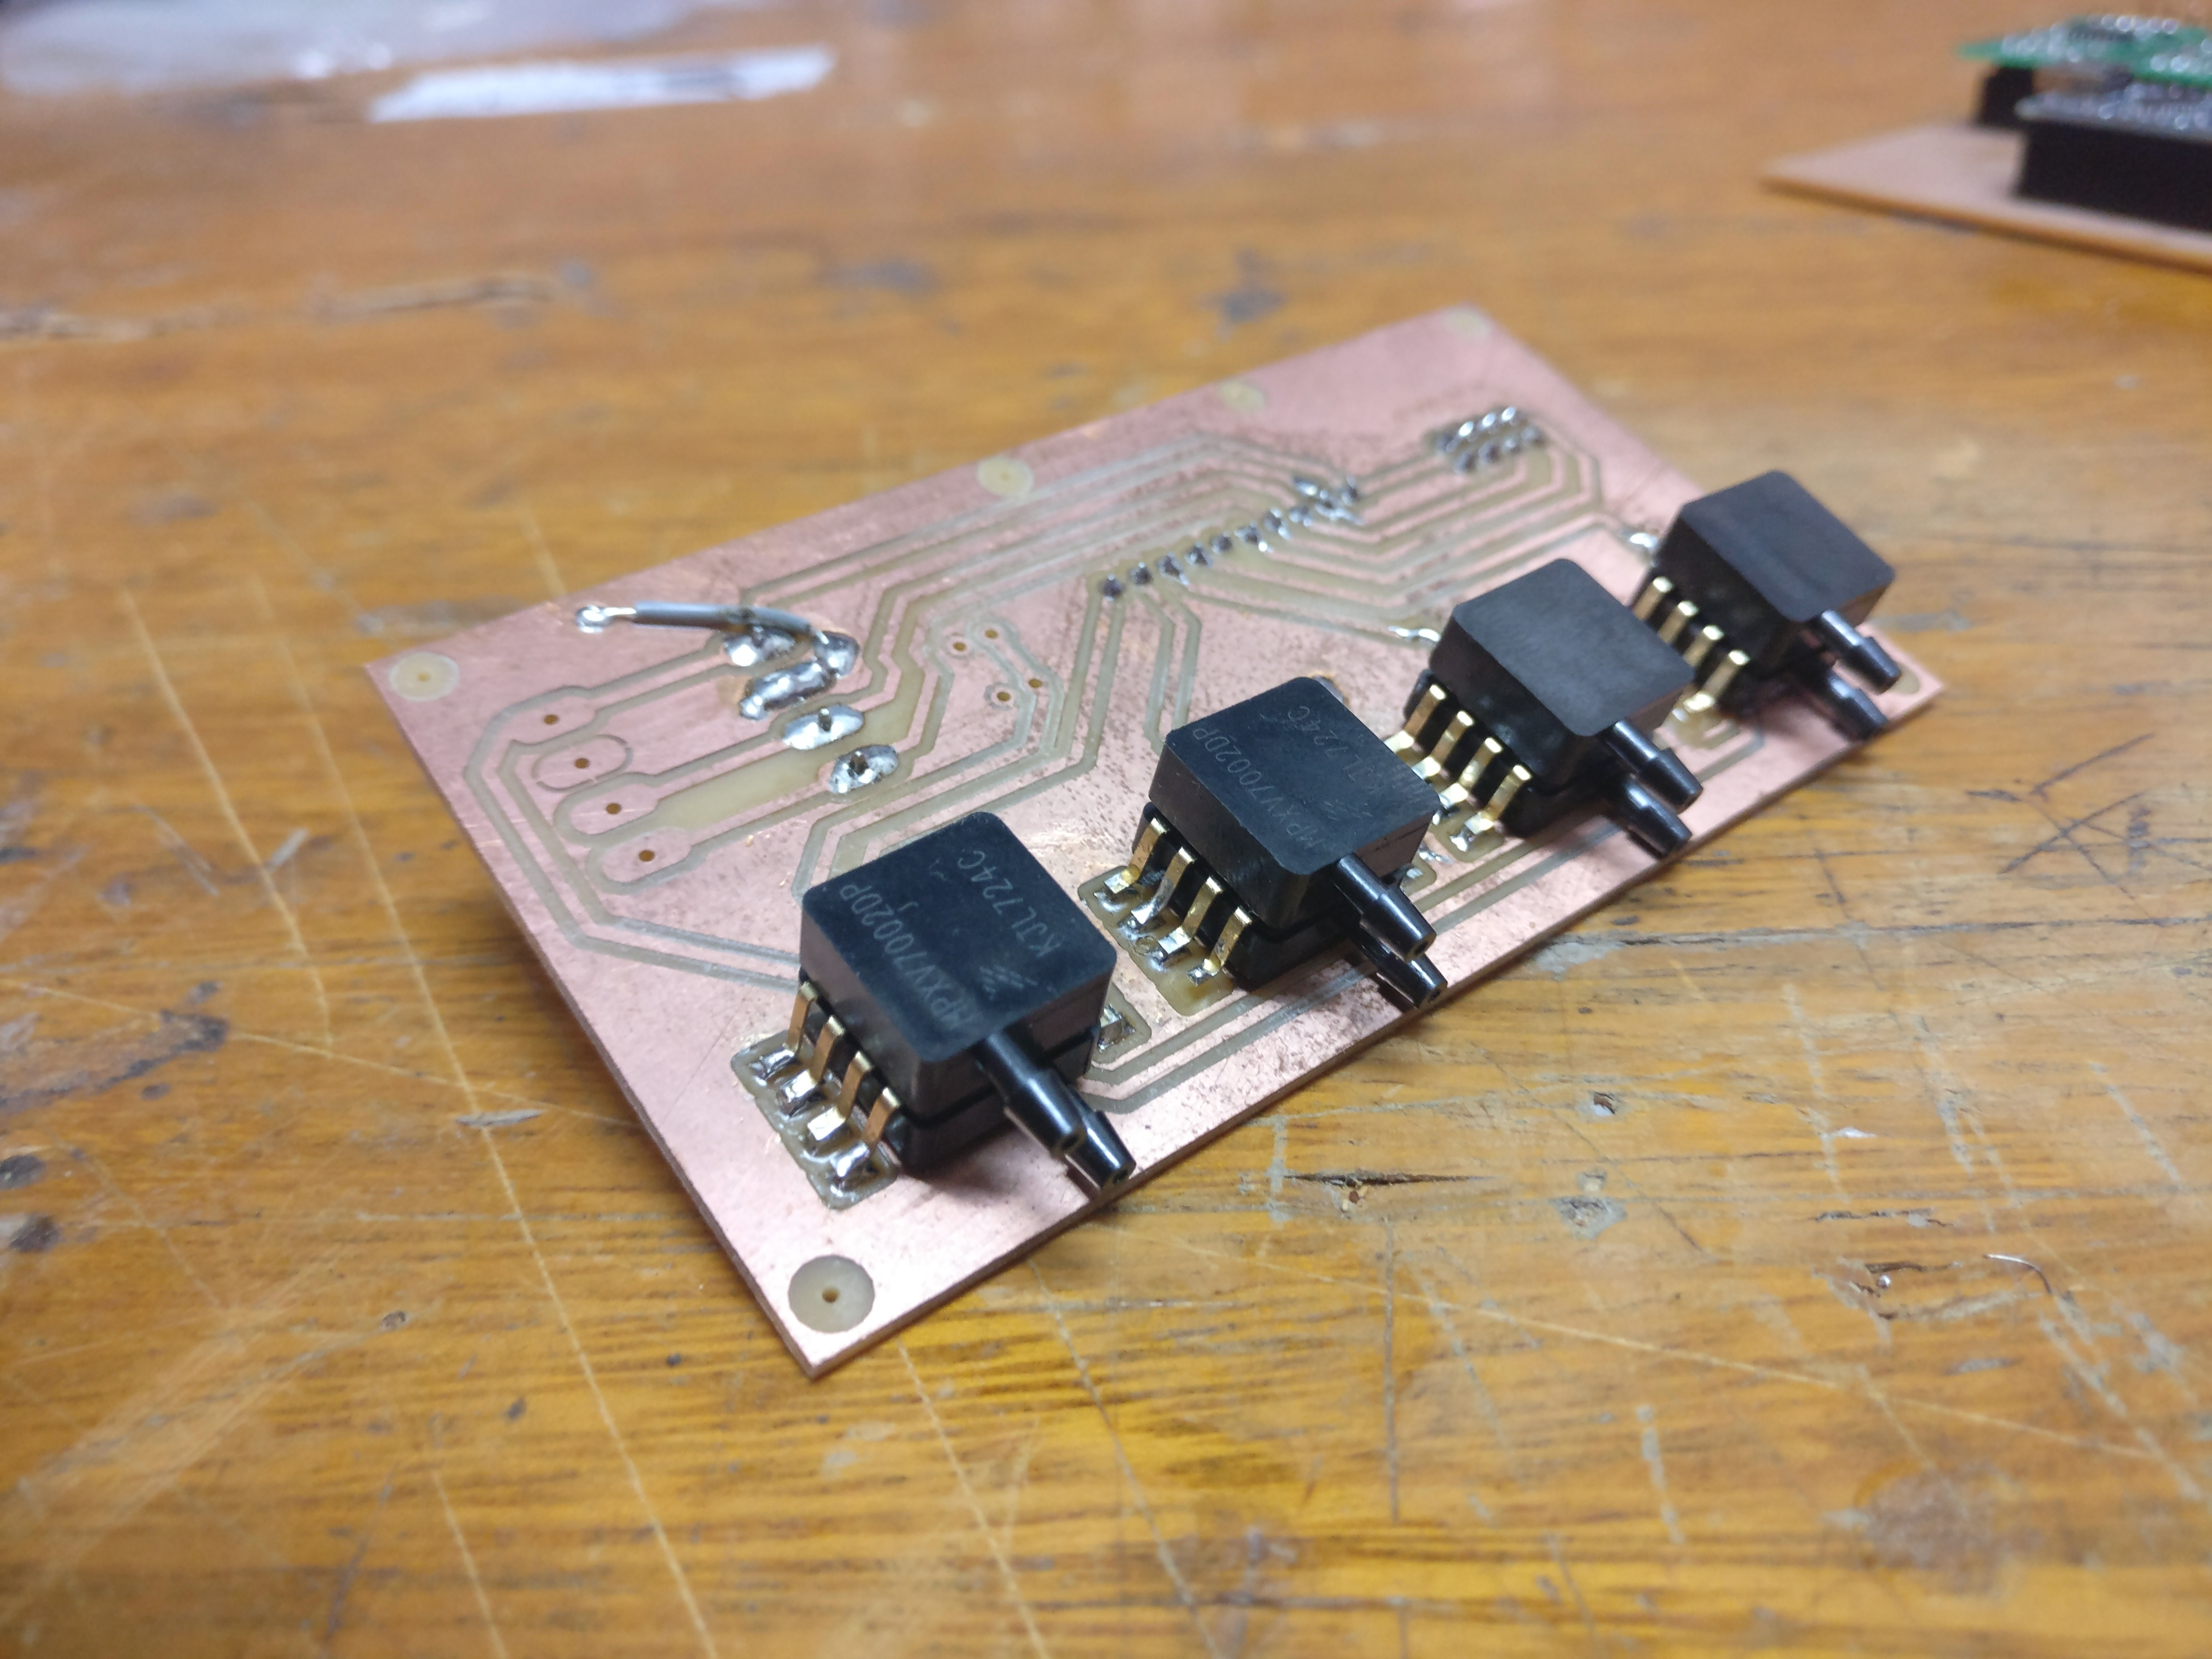
\includegraphics[width=.8\linewidth]{figuras/construcao/pcbs_montadas_2.jpg}
    \caption{Placa de transdutores de pressão diferencial fresada e com sensores instalados\cite{autor}.}
    \label{fig:placa_pcb_pitot}
\end{figure}

\begin{figure}[!ht]
    \centering
    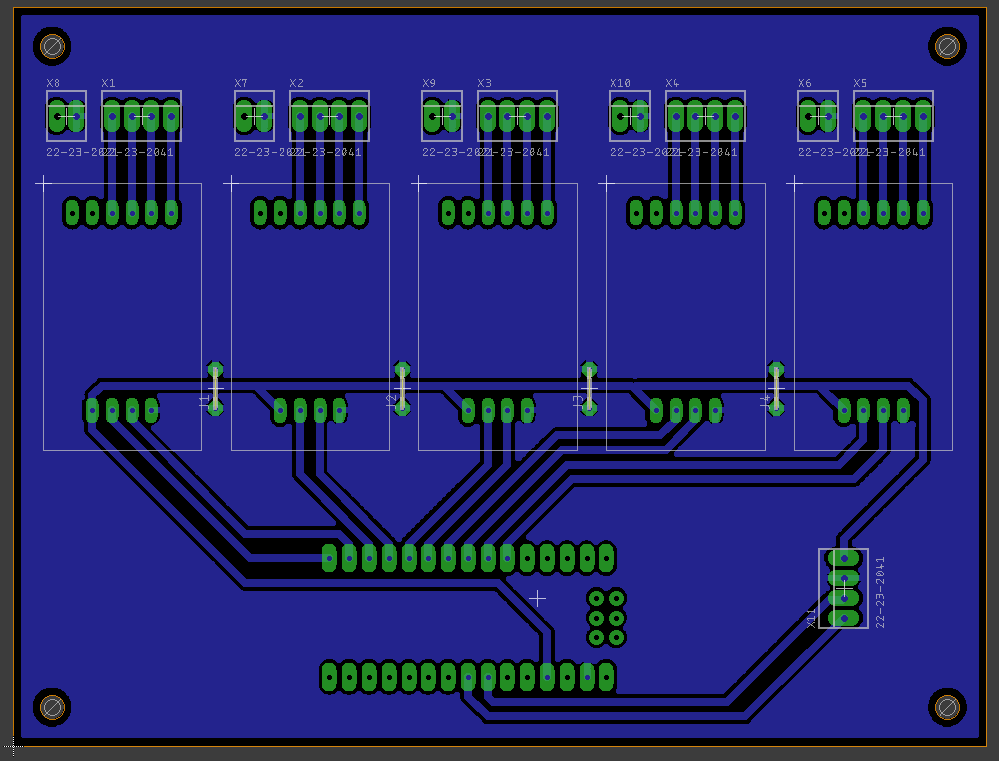
\includegraphics[width=.8\linewidth]{figuras/renders/loadcell_board.png}
    \caption{Projeto da placa de transdutores ce célula de carga no software Eagle\cite{autor}.}
    \label{fig:projeto_pcb_celulas}
\end{figure}

\begin{figure}[!ht]
    \centering
    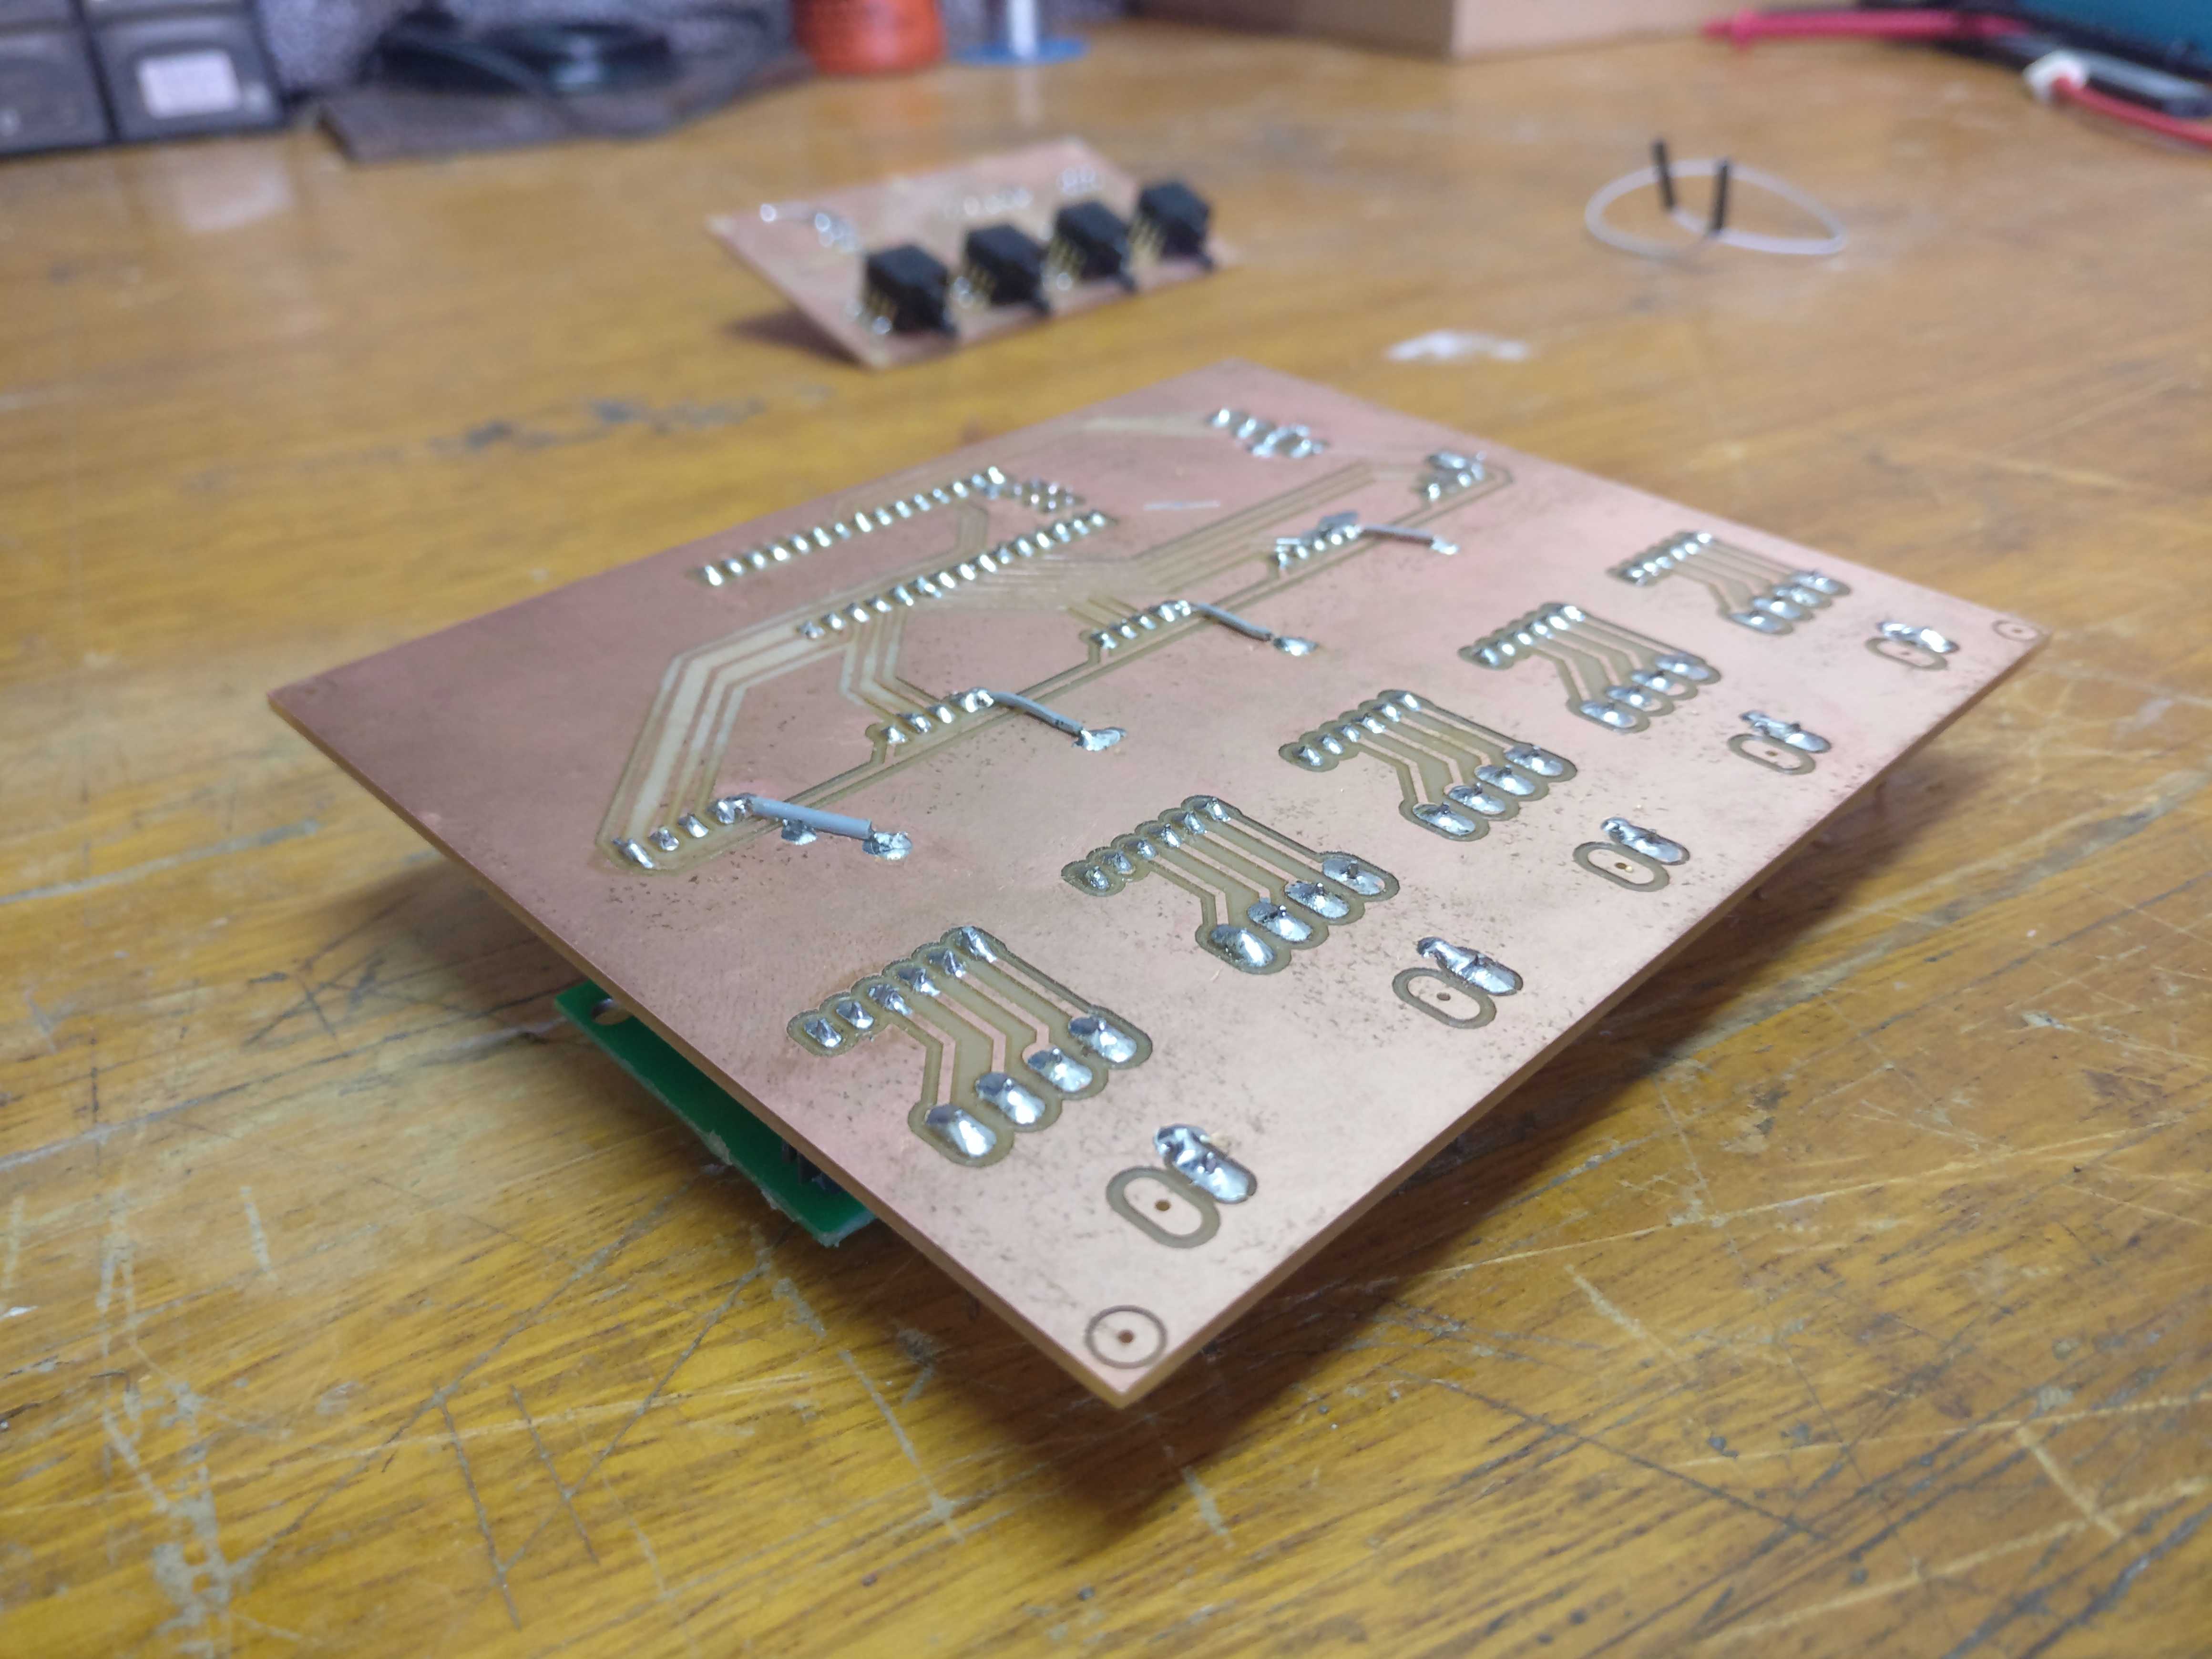
\includegraphics[width=.8\linewidth]{figuras/construcao/pcbs_montadas_3.jpg}
    \caption{Placa de transdutores de célula de carga fresada e com sensores instalados\cite{autor}.}
    \label{fig:placa_pcb_celulas}
\end{figure}

Foram confeccionados cases para alocação de ambas as placas e seus conectores. Os conectores usados neste projeto foram do modelo GX16, popularmente conhecidos como "conectores de aviação". Estes possuem trava rosqueada e ótimo contato elétrico. Os conectores ficam presos no case e não na placa, de modo que em caso de acidentes de tracionamento dos cabos as placas não sejam danificadas.

\begin{figure}[!ht]
    \centering
    
\includegraphics[width=.8\linewidth]{figuras/outras/placeholder.png}
    \caption{FOTO DOS CASES+PCB+CONECTORES\cite{autor}.}
    \label{fig:placeholder}
\end{figure}

\begin{figure}[!ht]
    \centering
    
\includegraphics[width=.8\linewidth]{figuras/outras/placeholder.png}
    \caption{FOTO DA CONEXAO INTERNA COM FIOS\cite{autor}.}
    \label{fig:placeholder}
\end{figure}

\subsection{Software Embarcado}

Como já mencionado, todo o software embarcado foi refatorado da versão MVP para esta primeira versão final. Alguns pontos principais merecem destaque:

\begin{itemize}
    \item Integração do Arduino como sensor na plataforma central, permitindo que mais Arduinos sejam conectados paralelamente de forma simplificada
    \item Implementação de nova rotina de ligação da bancada, adaptando automaticamente as configurações internas aos sensores que estiverem conectados, evitando a necessidade de alterar o código toda vez que um novo teste for executado
    \item Implementação de rotina de configuração do teste remotamente via app, permitindo que o operador inclua no arquivo de dados detalhes do teste como o dispositivo testado, seu angulo de incidência e outras condições, facilitando o entendimento dos dados pelo responsável por processa-los 
    \item Inclusão de código para uso da sonda de angulo de ataque através dos sensores de pressão diferencial
    \item Transferência de todas as configurações do software para um arquivo de configuração simplificada, permitindo que pessoas sem experiencia com o software embarcado consigam realizar configurações avançadas de forma simples
\end{itemize}

Sobre o primeiro ponto, na versão MVP o Arduino que fazia a aquisição do sinal das células não se comunicava com o Raspberry Pi (plataforma central). Deste modo, seus dados não possuíam sincronia, e esta deveria ser feita posteriormente por quem fosse se utilizar dos dados. Além de exigir um grande trabalho manual, este processo muitas vezes não ficava com qualidade satisfatória, e os dados acabavam não sincronizados. Para resolver este problema o Arduino passou a ser conectado na plataforma central e tratado por esta como um sensor, que responde a pedidos de envio de dados. Para garantir robustez na troca de dados foi implementado protocolo de comunicação de dois sentidos com confirmação de recebimento e checksum.  

\subsection{Software de Analise}

DESCREVER SOFTWARE DE ANALISE

\subsection{Sensoriamento}

\begin{itemize}
    \item Sonda de angulo de ataque
    \item IMU
\end{itemize}

\begin{figure}[!ht]
    \centering
    
\includegraphics[width=.8\linewidth]{figuras/outras/placeholder.png}
    \caption{SIMULACAO CFD\cite{autor}.}
    \label{fig:placeholder}
\end{figure}

Foram posicionados na bancada um tubo de Pitot e uma sonda de angulo de ataque. O tubo foi posicionado na bancada de forma a medir velocidade de fluxo livre (longe de distorções causadas pelo conjunto carro/bancada/componente). Para auxiliar neste posicionamento uma simulação qualitativa foi realizada em CFD utilizando o código Fluent, disponível na plataforma Ansys. A modelagem foi simplificada em pontos considerados não criticos de modo a evitar problemas de malha e acelerar a convergência dos resultados.

\begin{figure}[!ht]
    \centering
    
\includegraphics[width=.8\linewidth]{figuras/outras/placeholder.png}
    \caption{ESQUEMATICO DA DISPOSICAO DOS TUBOS DE PITOT\cite{autor}.}
    \label{fig:placeholder}
\end{figure}

A sonda de angulo de ataque deve ser fixada ao componente a ser testado, com alinhamento junto a linha de referencia horizontal do mesmo (i.e. linha de corda da raiz da asa). Este posicionamento permite que o angulo de ataque real seja medido pela sonda. 

Para o protótipo a ser testado foi confeccionado um suporte para a sonda, a ser instalado no bordo de ataque da asa. Suportes como este podem ser modelados e impressos rapidamente, e permitem um melhor alinhamento da sonda ao componente.

\begin{figure}[!ht]
    \centering
    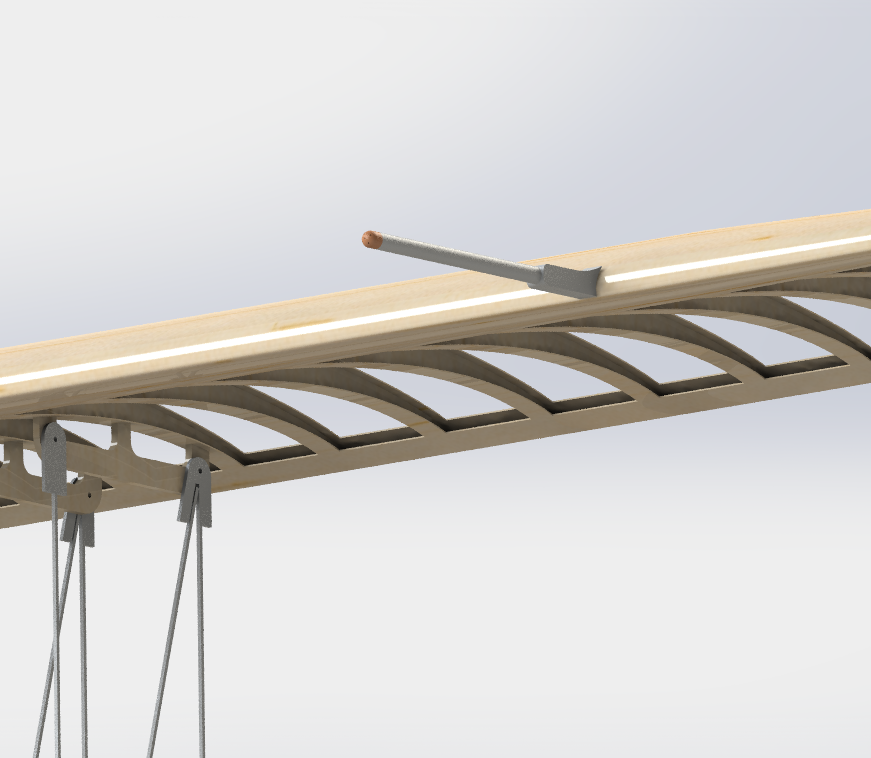
\includegraphics[width=.8\linewidth]{figuras/renders/sonda_aoa_asa_superior.png}
    \caption{Detalhe do Pitot de multiplas tomadas (sonda de angulo de ataque) montada na asa superior da aeronave testada\cite{autor}.}
    \label{fig:placeholder}
\end{figure}

\subsection{Bancada final}

As figuras \ref{fig:render_bancada_completa} e \ref{fig:bancada_construida} mostram a modelagem final da bancada e mesma construída.

\begin{figure}[!ht]
    \centering
    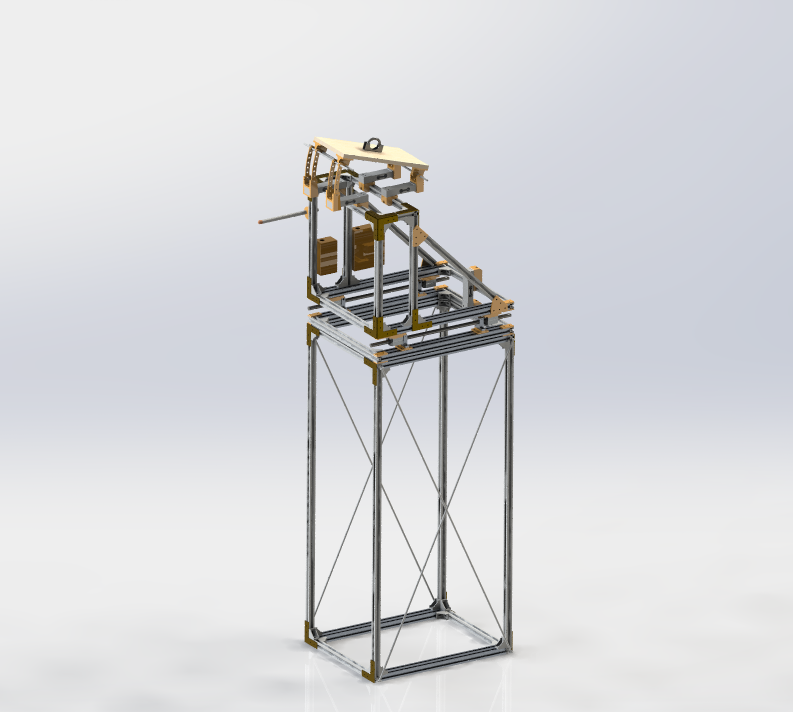
\includegraphics[width=.8\linewidth]{figuras/renders/perspectiva_sem_asa_com_pitot.png}
    \caption{Renderização da bancada modelada no software Solidworks 2016\cite{autor}.}
    \label{fig:render_bancada_completa}
\end{figure}

\begin{figure}[!ht]
    \centering
    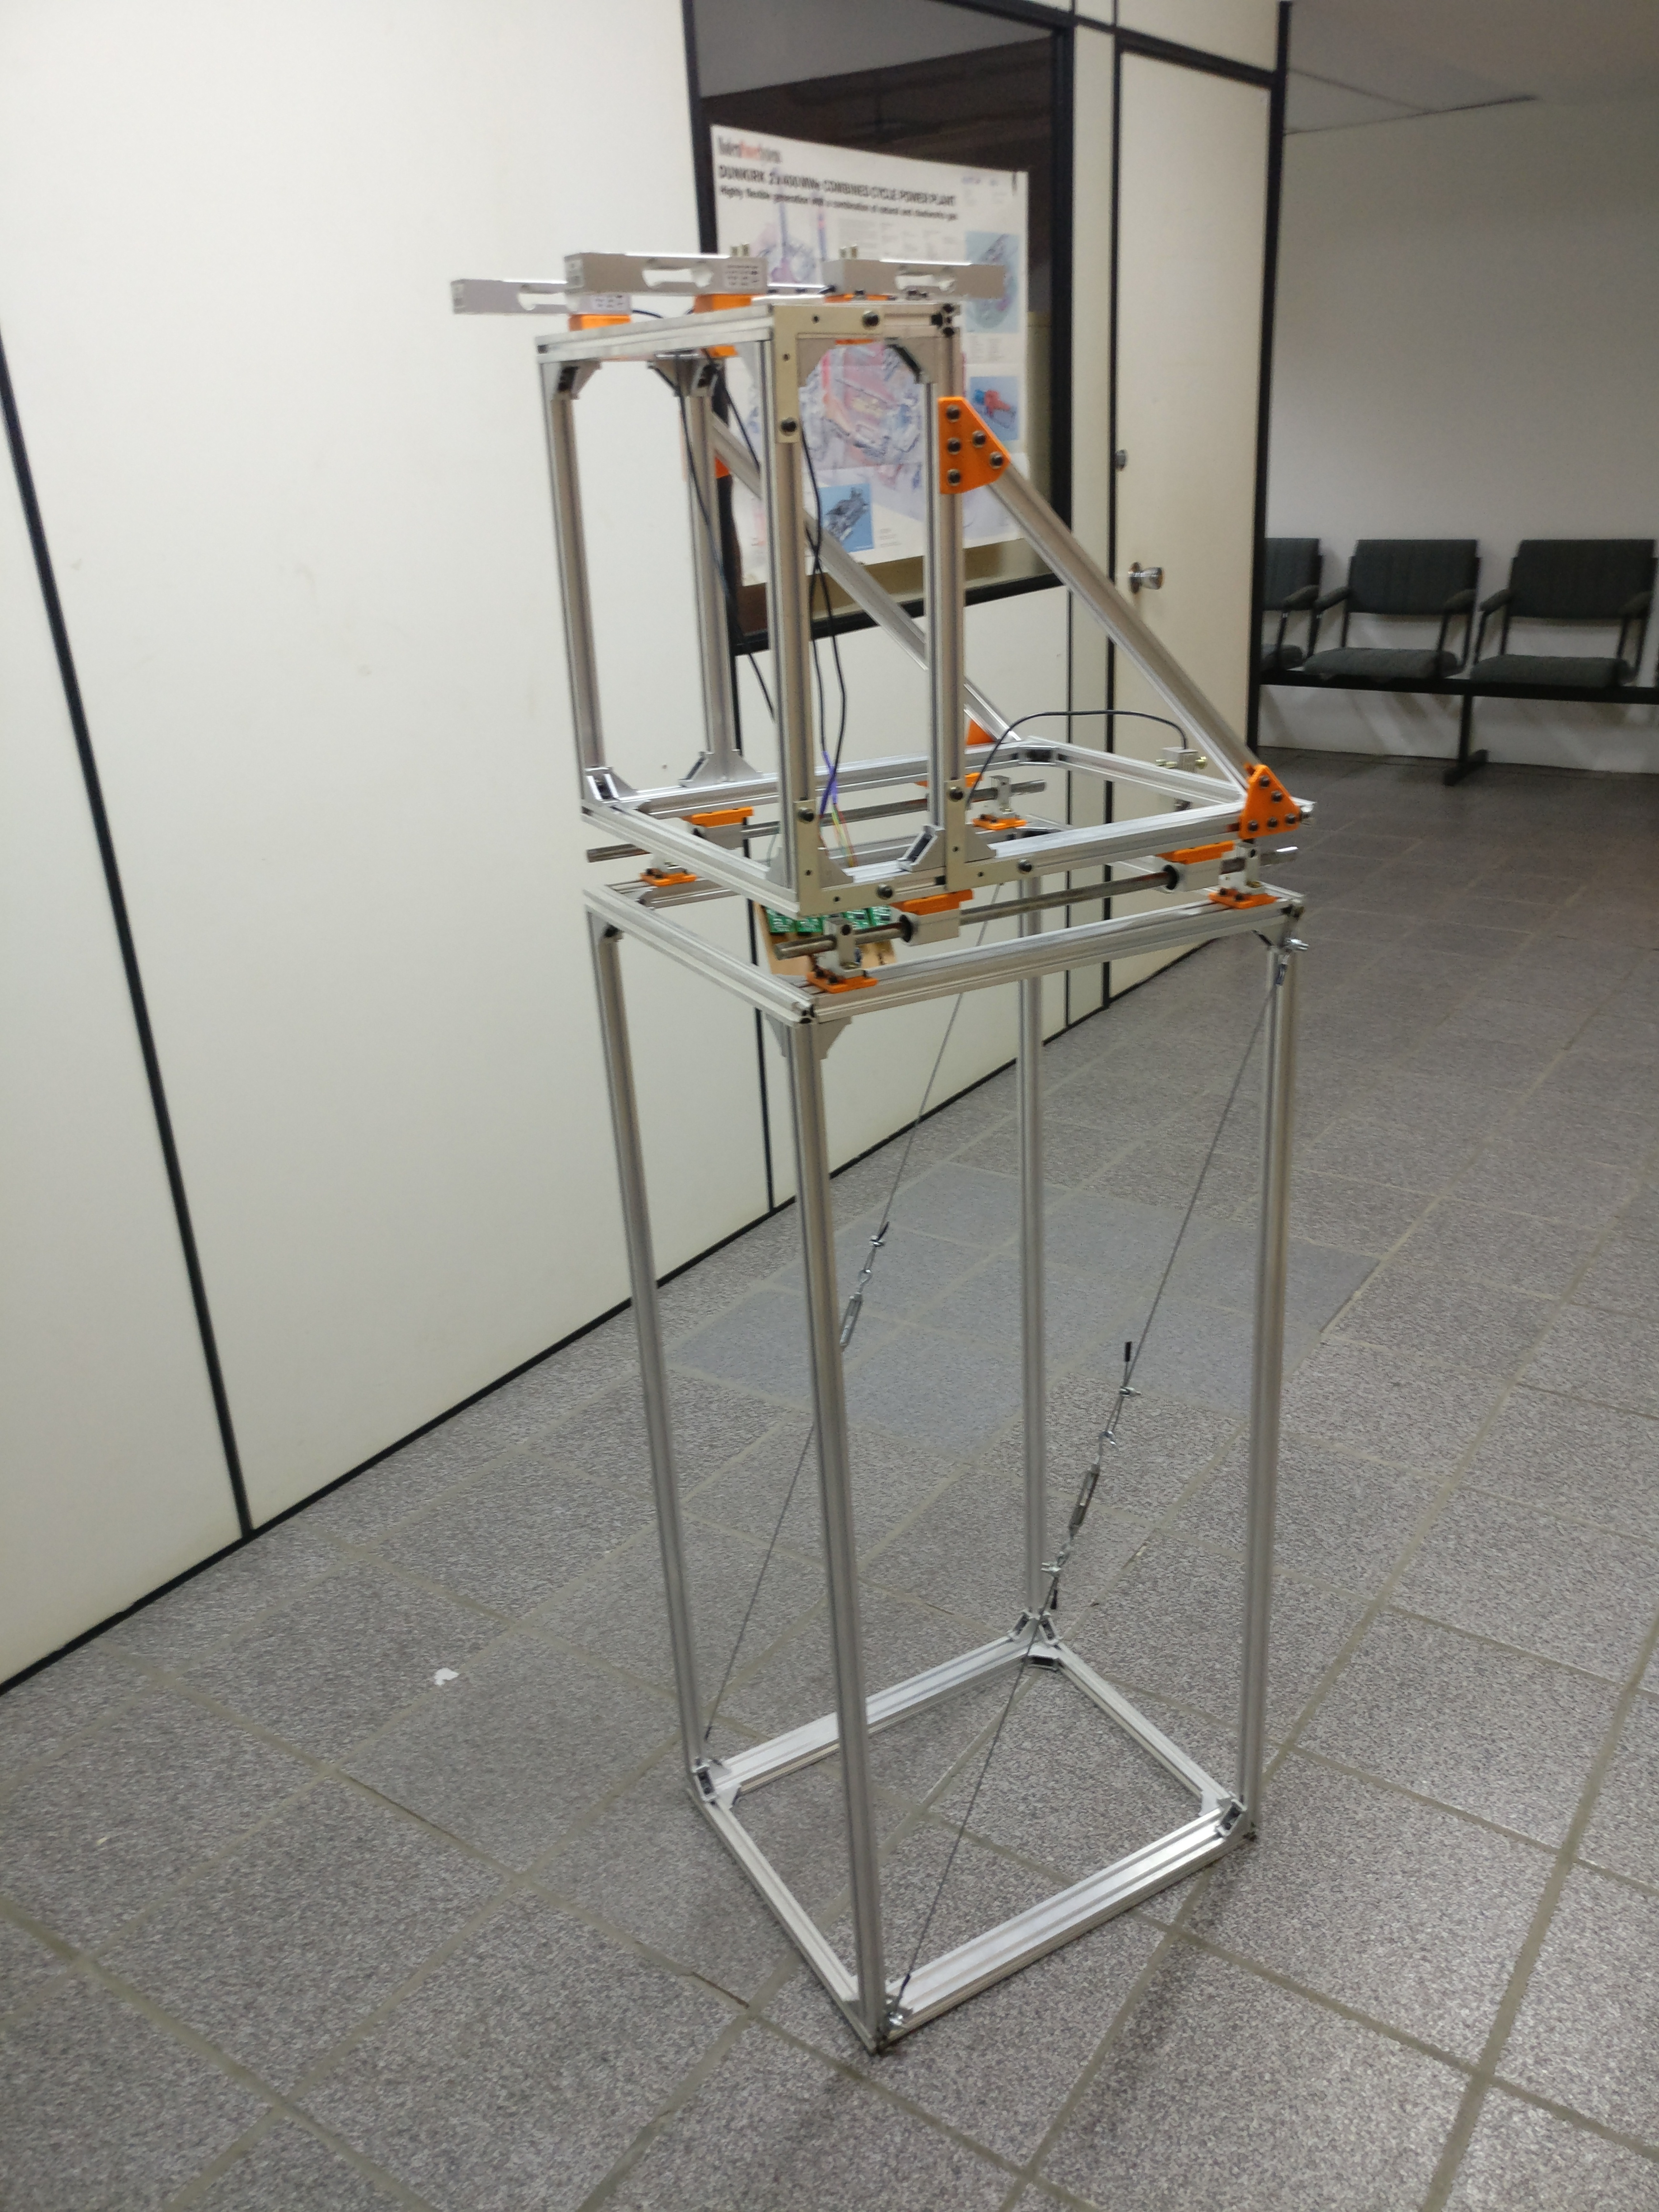
\includegraphics[width=.8\linewidth]{figuras/construcao/bancada_inteira.jpg}
    \caption{Foto da bancada construída\cite{autor}.}
    \label{fig:bancada_construida}
\end{figure}



\section{Testes}

Uma serie de testes foi realizada inicialmente de forma mais rápida visando-se buscar melhorias a serem feitas na bancada, seja na parte mecânica, eletrônica ou de software. Estes testes se deram simultaneamente ao projeto e foram responsáveis por melhorias como:

\begin{enumerate}
    \item Verificação da necessidade de simulação da bancada para otimização da posição do tubo de Pitot.
    \item Verificação da calibração das células de carga e tubos de Pitot.
    \item Inclusão da possibilidade de zeragem das células e Pitots ao inicio do teste via app
    \item Inclusão da IMU para medição das acelerações sofridas durante o teste.
    \item Verificação da necessidade de uso da sonda acoplada ao componente a ser testado
\end{enumerate}

Uma vez finalizada a versão final da bancada, foi iniciada a condução dos testes comparativos.

\subsection{O dispositivo de teste}

Os testes comparativos tem por finalidade gerar dados sobre geometrias conhecidas que possam ser confrontados com literatura existente. Para este teste o dispositivo ideal seria uma asa utilizando perfis do tipo NACA, que possuem vasta literatura de dados experimentais, porém devido a problemas orçamentários e de tempo não foi possível a construção de tal dispositivo, sendo o teste realizado com a asa do primeiro protótipo da equipe para o ano de 2019. A geometria desta asa se encontra a seguir:

\begin{table}[]
\centering
\begin{tabular}{lll}
 & 1a Seçao & 2a Seçao \\
Perfil & Selig1223 & Selig1223 \\
Envergadura & X & X \\
Corda na raiz & X & X \\
Corda na ponta & X & X
\end{tabular}
\end{table}

Foi escolhida a velocidade de X m/s para os testes, visto que é a velocidade de cruzeiro da aeronave. O Reynolds referente a Corda Média Aerodinâmica da asa é de X para as condições do teste.

\begin{figure}[!ht]
    \centering
    
\includegraphics[width=.8\linewidth]{figuras/outras/placeholder.png}
    \caption{MODELAGEM COM DIMENSOES DA ASA 2019.\cite{autor}.}
    \label{fig:placeholder}
\end{figure}

Para a simulação de tal asa foi utilizado o software de código-aberto AVL, que implementa o algoritmo Vortex Lattice Method.

\begin{figure}[!ht]
    \centering
    
\includegraphics[width=.8\linewidth]{figuras/outras/placeholder.png}
    \caption{RENDERING DA SIMULACAO NO AVL\cite{autor}.}
    \label{fig:placeholder}
\end{figure}

A asa foi confeccionada com nervuras em MDF 6mm, detalhes em madeira balsa, com laminaçao de fibra de carbono nas areas com maiores solicitaçoes, conceito estrutural de caixa de torçao e entelamento com fita Adelbras. Simulações estruturais para tal asa foram realizadas buscando-se avaliar a torçao geométrica e a deflexão desenvolvidas durante sua operação. Uma torçao máxima de X graus e um deslocamento de ponta máximo de X mm foram encontrados. Segundo X, a perda de sustentação para tal condição seria de X, valor baixo e portanto ignorado durante a avaliação dos resultados.

\begin{figure}[!ht]
    \centering
    
\includegraphics[width=.8\linewidth]{figuras/outras/placeholder.png}
    \caption{FOTO DA ASA CONSTRUIDA\cite{autor}.}
    \label{fig:placeholder}
\end{figure}

\subsection{O teste}

Os testes foram conduzidos em uma avenida reta e comprida (Avenida Beira-mar Norte), excencialmente plana e em horário de trânsito reduzido (durante a madrugada).

\begin{figure}[!ht]
    \centering
    \includegraphics[width=.8\linewidth]{figuras/internet/here_open_street_maps.png}
    \caption{Local onde foram realizados os testes\cite{autor}.}
    \label{fig:mapa_teste}
\end{figure}

O teste foi conduzido acelerando-se o carro até uma velocidade de aproximadamente 15m/s (54km/h) e mantendo essa velocidade durante o maior tempo possível. Sendo conduzido desta maneira o teste entrega resultados para apenas um valor de Reynolds. Foi assim feito pois em testes preliminares verificou-se que cada bateria de testes demorava um tempo considerável, e repetir ela para uma grande faixa de Reynolds reduziria o numero de dados para cada velocidade. Decidiu-se portanto ter um maior numero de dados para um mesmo Reynolds, garantindo-se uma qualidade melhor dos resultados finais. Com mais tempo porem, ou uma condução mais rápida dos testes, poder-se-ia (sdds presidento) realizar os testes para mais valores de Reynolds.  

\begin{figure}[!ht]
    \centering
    \includegraphics[width=.8\linewidth]{figuras/outras/placeholder.png}
    \caption{FOTO DO APP SENDO USADO\cite{autor}.}
    \label{fig:placeholder}
\end{figure}

Para se averiguar a velocidade foram utilizados dois recursos: velocímetro do próprio carro e velocidade medida pelo pelos tubos de Pitot. Idealmente as duas medidas devem apresentar resultado semelhante. Para se acompanhar a velocidade medida pelos Pitots em tempo real foi utilizado o aplicativo desenvolvido.

\begin{figure}[!ht]
    \centering
    \includegraphics[width=.8\linewidth]{figuras/testes/teste_aviao_completo.JPG}
    \caption{Foto do teste com aeronave Céu Azul 2019 P1\cite{autor}.}
    \label{fig:foto_teste_aviao}
\end{figure}

\begin{figure}[!ht]
    \centering
    \includegraphics[width=.8\linewidth]{figuras/outras/placeholder.png}
    \caption{FOTO DO TESTE - 2\cite{autor}.}
    \label{fig:placeholder}
\end{figure}

\begin{figure}[!ht]
    \centering
    \includegraphics[width=.8\linewidth]{figuras/outras/placeholder.png}
    \caption{FOTO DO TESTE - 3\cite{autor}.}
    \label{fig:placeholder}
\end{figure}

Para cada bateria de testes a asa foi instalada em um ângulo de incidência diferente. Foram realizados testes para os ângulos de 0, 3, 6, 9, 12 e 15 graus. Para cada um dos ângulos, três baterias de teste foram conduzidas, buscando-se criar uma base de dados grande e diminuir a influencia dos testes nos resultados.


\chapter{Resultados}\label{chp:res}

O conjunto de dados, originais e derivados (aqueles criados a partir de dados originais), estão apresentados na tabela \ref{tab:all_data_table}.

\begin{table}[]
\centering
\resizebox{\textwidth}{!}{\begin{tabular}{|l|c|c|c|c|}
\hline
Plataforma & \multicolumn{4}{c|}{Dado} \\ \hline
 & \multicolumn{4}{l|}{} \\ \hline
Sensor & Tempo & Mensagem & Tamanho do arquivo \\ \hline
Giroscopio & Taxa de giro em X & Taxa de giro em Y & Taxa de giro em Z &  \\ \hline
Acelerometro & Aceleração em X & Aceleração em Y & Aceleração em Z &  \\ \hline
Pitot & Raw Pitot - Pitot 0 & Pressao Dinamica Ref.- Pitot 0 (virtual) & Velocidade Ref. - Pitot 0 (virtual) &  \\ \hline
Pitot & Raw Pitot - Pitot 1 & Pressao Dinamica Ref.- Pitot 1 (virtual) & Velocidade Ref. - Pitot 1 (virtual) &  \\ \hline
Pitot & Raw Pitot - Pitot 2 & Pressao Dinamica Ref.- Pitot 2 (virtual) & Velocidade Ref. - Pitot 2 (virtual) &  \\ \hline
Pitots & AoA Differential Pressure - Sonda AoA (virtual) 0 & AoA Dynamic Pressure - Sonda AoA 0 (virtual) & AoA - Sonda AoA 0 (virtual) &  \\ \hline
Célula de carga & Raw Cell Data - Celula Horizontal & Forca - Celula Horizontal (virtual) &  &  \\ \hline
Célula de carga & Raw Cell Data - Celula Frontal Direita & Forca - Celula Frontal Direita (virtual) &  &  \\ \hline
Célula de carga & Raw Cell Data - Celula Frontal Esquerda & Forca - Celula Frontal Esquerda (virtual) &  &  \\ \hline
Célula de carga & Raw Cell Data - Celula Traseira Direita & Forca - Celula Traseira Direita (virtual) &  &  \\ \hline
Célula de carga & Raw Cell Data - Celula Traseira Esquerda & Forca - Celula Traseira Esquerda (virtual) &  &  \\ \hline
Células de carga e Pitots & Lift (virtual) & Drag (virtual) & Moment (virtual) & Distance Cp (virtual) \\ \hline
\end{tabular}}
\caption{Dados disponíveis no arquivo gerado pela plataforma de aquisição}
\label{tab:all_data_table}
\end{table}

Na imagem \ref{fig:raw_accel_plots} pode ser visto um exemplo dos dados adquiridos durante uma bateria de testes. A gravação dos dados na plataforma ocorre a uma taxa fixa de 100 Hz, diferente da taxa original de aquisição de cada sensor. 

Isso é feito de modo que todos apresentem uma mesma frequência de ocorrência na plataforma e portanto tenham sempre correspondência nos dados dos outros sensores, facilitando posterior processamento. Neste nivelamento alguns dados, por possuírem frequência de aquisição mais baixa que a de gravação da plataforma, acabam se repetindo até que novos valores estejam disponíveis.

\begin{figure}[!ht]
    \centering
    \includegraphics[width=.8\linewidth]{plots/accel_plots.pdf}
    \caption{Exemplo de dados do acelerômetro. Fonte: O autor.}
    \label{fig:raw_accel_plots}
\end{figure}

\begin{figure}[!ht]
    \centering
    \includegraphics[width=.8\linewidth]{plots/gyro_plots.pdf}
    \caption{Exemplo de dados do giroscópio. Fonte: O autor.}
    \label{fig:raw_gyro_plots}
\end{figure}

\begin{figure}[!ht]
    \centering
    \includegraphics[width=.8\linewidth]{plots/pitot_plots.pdf}
    \caption{Exemplo de dados do Pitot. Fonte: O autor.}
    \label{fig:raw_pitot_plots}
\end{figure}

\begin{figure}[!ht]
    \centering
    \includegraphics[width=.8\linewidth]{plots/aoa_plots.pdf}
    \caption{Exemplo de dados da sonda de angulo de ataque. Fonte: O autor.}
    \label{fig:raw_aoa_plots}
\end{figure}

\begin{figure}[!ht]
    \centering
    \includegraphics[width=.8\linewidth]{plots/loads_plots.pdf}
    \caption{Exemplo de dados de cargas aerodinâmicas. Fonte: O autor.}
    \label{fig:raw_load_plots}
\end{figure}

\section{Limpeza, filtragem e redução dos dados}

\subsection{Limpeza de dados}

Dado que o teste foi executado procurando-se atingir uma velocidade constante, o resultado final será dado para apenas um valor de Reynolds, sendo assim, dados adquiridos que sejam válidos mas não estejam próximos ao Reynolds do teste não devem ser utilizados, dado que devem apresentar comportamento aerodinâmico diferente daquele correspondente ao Reynolds desejado \citep{anderson1984fundamentals}. Sendo assim, a primeira limpeza a ser realizada é quanto à faixa de interesse de Reynolds. Desta forma os dados a serem utilizados para medição serão aqueles correspondentes aos instantes onde foi alcançada a velocidade estipulada para o teste, com desvio máximo de 10\%.

Para mostrar o resultado desta filtragem usaremos os dados de Sustentação. Os dados originais se encontram na figura \ref{fig:orig_lift_plot} enquanto os dados após filtragem por faixa de Reynolds se encontram na figura \ref{fig:lift_reynolds_filter} :

\begin{figure}[!ht]
    \centering
    \includegraphics[width=.8\linewidth]{plots/orig_lift_plot.pdf}
    \caption{Dados de sustentação e velocidade originais. Fonte: O autor.}
    \label{fig:orig_lift_plot}
\end{figure}


\begin{figure}[!ht]
    \centering
    \includegraphics[width=.8\linewidth]{plots/reynolds_lift_plot.pdf}
    \caption{Dados de sustentação e velocidade após filtragem pela faixa de Reynolds do teste (1o patamar). Fonte: O autor.}
    \label{fig:lift_reynolds_filter}
\end{figure}

% A premissa principal para o uso dos dados do teste é de que os valores medidos estejam dentro do intervalo de uso dos sensores e de que as acelerações sobre o sistema sejam baixas. O intervalo de uso dos sensores se encontra na tabela X.

% \begin{table}[!ht]
%     \centering
%     \includegraphics[width=.8\linewidth]{figuras/outras/placeholder.png}
%     \caption{TABELA COM ZONA DE USO DE CADA SENSOR. Fonte: O autor.}
%     \label{fig:placeholder}
% \end{table}

% Após a seleção por faixa de Reynolds, dados fora da faixa de medição dos sensores e dados com aceleração em X, Y ou Z maior que 0.5g foram também descartados.

\subsection{Filtragem}

Após a limpeza dos dados, onde foram removidos aqueles que estavam fora da zona de interesse, buscou-se avaliar a filtragem do sinal, visando aumentar a relação sinal-ruido.

Primeiramente foram realizadas Transformadas Rápidas de Fourier nos dados das células e das sondas de angulo de ataque (incluindo velocidade). Através da transformação para o domínio da frequência foi possível encontrar as frequências de corte ideais para aplicação de filtros passa-baixa em cada um dos dados.

% \begin{figure}[!ht]
%     \centering
%     \includegrapha apoliics[width=.8\linewidth]{figuras/outras/placeholder.png}
%     \caption{ANALISES FFT. Fonte: O autor.}
%     \label{fig:fft_analysis}
% \end{figure}

% A partir do resultado das analises foram dimensionados filtros do tipo passa-baixa para a remoção dos ruídos de alta frequência em cada um dos dados.

% As frequências de corte para cada dado se encontram na tabela X. 

% \begin{table}[!ht]
%     \centering
%     \includegraphics[width=.6\linewidth]{figuras/outras/placeholder.png}
%     \caption{TABELA COM FREQUENCIA DE CORTE DE CADA DADO. Fonte: O autor.}
%     \label{tab:cut_frequency_values}
% \end{table}

A titulo de exemplo, o resultado após filtragem para os dados de sustentação e velocidade se encontram na figura \ref{fig:filtered_lift_plot}.

\begin{figure}[!ht]
    \centering
    \includegraphics[width=.8\linewidth]{plots/filtered_lift_plot.pdf}
    \caption{Dados de sustentação e velocidade após filtragem das altas frequências. Fonte: O autor.}
    \label{fig:filtered_lift_plot}
\end{figure}

\subsection{Redução}

Em posse dos dados filtrados passa-se à etapa de redução. Não é do interesse do projetista a principio saber qual sustentação, arrasto ou momento foram alcançados durante os testes, pois esses são dados absolutos que dependem do tamanho do componente e da velocidade no instante medido. Para facilidade de analise e mais justa comparação entre diferentes componentes é de interesse a redução destes dados na forma dos coeficientes aerodinâmicos \citep{anderson1984fundamentals}.

\begin{equation}
    C_L =  \frac{L}{ \frac{1}{2} \rho V^{2} S}
    \label{eq:cl}
\end{equation}

\begin{equation} 
    C_D =  \frac{D}{ \frac{1}{2} \rho V^{2} S}
    \label{eq:cd}
\end{equation}

\begin{equation}
    C_M =  \frac{M}{ \frac{1}{2} \rho V^{2} S C_{M.A.}} 
    \label{eq:cm}
\end{equation}

As equações \ref{eq:cl}, \ref{eq:cd} e \ref{eq:cm} foram aplicadas a todas as amostras de dados gerando três novas colunas, $C_L$, $C_D$ e $C_M$, que podem ser visualizadas na figura \ref{fig:coefficients_plot}. Os dados das baterias de testes foram então condensados num mesmo conjunto de dados,para o qual então foram calculados o valor médio e o desvio padrão de cada coeficiente, para cada angulo de incidência.

\begin{figure}[!ht]
    \centering
    \includegraphics[width=.8\linewidth]{plots/coefficients_plot.pdf}
    \caption{Variação dos coeficientes aerodinâmicos ao longo do tempo para o patamar avaliado. Fonte: O autor.}
    \label{fig:coefficients_plot}
\end{figure}

Os valores finais de media para os coeficientes de cada angulo de incidência estão explicitados nos gráficos da figura \ref{fig:coefficients_alpha_plot}.

\begin{figure}[!ht]
    \centering
    \includegraphics[width=.8\linewidth]{plots/cl_cd_polar_medicao.png}
    \caption{Curvas $C_x vs Alpha$, experimental e simulado. Fonte: O autor.}
    \label{fig:coefficients_alpha_plot}
\end{figure}

Os resultados do teste demonstram um alto desvio entre os valores de sustentação medidos experimentalmente e os simulados. Já os dados de arrasto se encontram próximos entre as duas fontes, porém com os dados experimentais sendo sempre menores que os simulados, ao contrario do que normalmente se espera, dado que os métodos de VLM costumam subestimar o arrasto.

Estes testes se mostraram inconclusivos, indicando apenas que existe pelo menos uma fonte de erro. Este erro pode estar vindo da própria bancada, por alguma falha construtiva ou de calibração, da execução do teste, por exemplo angulando-se o profundor de valor diferente do simulado, ou mesmo do protótipo, por falhas na construção. 

De fato tal aeronave indicou em testes de voo posteriores estar aparentemente com uma relação $C_L/C_D$ mais baixa do que o esperado, não conseguindo decolar com cargas maiores que 70\% daquela estimada em projeto, além de apresentar assimetria de sustentação entre os dois lados da asa, indicando diminuição da sustentação total gerada com relação aquela estimada em projeto.

Além disso os dados coletados aparentaram boa qualidade e relativa estabilidade, além de apresentarem comportamento coerente com o esperado. Erros na angulação do profundor, mesmo que altas, também não acarretariam em desvio tao grande dos valores de sustentação. Deste modo, parece provável um desvio do próprio protótipo em relação ao simulado, porém é importante que fique claro que tal hipótese não pode ser comprovada, dado que a bancada não foi validada contra valores conhecidos de literatura.


 % Texto do cap4.tex
\chapter{Conclusão}\label{chp:conc}

    Este trabalho procurou descrever o projeto, construção e teste de uma bancada experimental para caracterização aerodinâmica de componentes de VANTs, visando eliminar a necessidade de testes em túnel de vento ou ensaios em voo.
    
    O trabalho foi desenvolvida no âmbito de uma equipe de projeto aeronáutico, buscando preencher a necessidade da mesma por dados experimentais que norteassem a validação e otimização de seus projetos.
    
    O trabalho foi bem sucedido no sentido de projetar, construir e testar tal bancada, cumprindo os requisitos estabelecidos de custo, facilidade de uso, desenvolvimento de softwares de suporte e documentação. 
    
    Os resultados obtidos no teste estão dentro do esperado quando comparados as simulações para os mesmos componentes testados.  Não foram testados contudo componentes com valores experimentais conhecidos, de forma que não se pode dizer que a bancada esta validada. Esperava-se ao inicio deste trabalho validar ou invalidar a bancada, porém a necessidade de finalizar os ensaios experimentais antes do previsto impediu que tal ação fosse concluída.
    
    Durante o desenvolvimento deste trabalho, dificuldades surgiram onde se poderia e onde não se poderia imaginar. Atrasos na entrega dos componentes, cargas não previstas, erros na execução dos testes, comportamentos inesperados do software de aquisição de dados, comportamentos inesperados dos sensores, todos foram problemas encontrados durante o caminho, felizmente resolvidos, um a um, ainda que atrasando o cronograma previsto.
    
    O uso da bancada hoje se encontra bastante facilitado, sendo possível realizar os testes e a analise dos resultados em uma noite de trabalho, considerando um bom planejamento e execução dos mesmos.
    
\section{Trabalhos futuros}
    
    Pode-se dizer que este trabalho se encontra em estagio avançado, mas ainda não concluído. A principal necessidade que se enxerga para um trabalho futuro é a validação da mesma para componentes já experimentalmente caracterizados. Esta validação agregaria em muito e permitiria que a equipe Céu Azul passasse a realizar seus ensaios experimentais visando otimizar o projeto com uma maior garantia sobre a validade dos resultados. Além da própria validação, alguns pontos a se tratar no futuro, seja por este autor ou por um terceiro, são levantados:
    
\begin{itemize}
    \item Mudança na solução da bandeja inferior da balança, passando a utilizar 3 células de carga e eliminando as guias lineares.
    \item Calibração dos fatores de acoplamento entre medições de sustentação e arrasto
    \item Validação da bancada contra geometrias com valores experimentais já consolidados, tais como esferas, cilindros e asas de perfil NACA
    \item Desenvolvimento de interface gráfica para carregamento dos dados de testes, visando eliminar a necessidade de execução das analises via scripts.
    \item Inclusão de rotina de calibração das células de carga e dos tubos de Pitot via app, tornando a calibração um processo rápido e facilitado.
    \item Inclusão de rotina de testes de forma guiada pelo app, isto é, em um formato de passo-a-passo, com instruções de execução, avisos de mal-uso ou resultados inconsistentes e automatização das analises.
    \item Possibilidade de transferência dos dados da plataforma de aquisição para o celular via Bluetooth, eliminando a necessidade de retirada do cartão de memoria da mesma.
    \item Inclusão de modo de gravação de áudio no app, visando a possibilidade de uma "narração" do teste pelo responsável. Este áudio permitiria que avaliações extras pudessem ser realizadas pelo responsável pela analise, como identificação de possíveis erros de execução, anormalidades ou mesmo testes diferenciados, como a execução de comandos na aeronave a serem posteriormente caracterizados. 
\end{itemize}
 % Texto do cap5.tex



%%%%%%%%%%%%%%%%%%%%%%%%%%
%%Elementos Pós-Textuais%%
%%%%%%%%%%%%%%%%%%%%%%%%%%
%%--------Bibliografia--------
\Bibliografia{referenciasbibliograficas} % arquivo bibtex com as referências (referenciasbibliograficas.bib)

%%--------Apêndice--------
%% Descomente caso exista a necessidade da inclusão de apêndices
%\apendice % Comando que inclui os apêndices
%\include{7_Apendice/apendice_1}   % Arquivo apendice_1.tex
%\include{7_Apendice/apendice_2}   % Arquivo apendice_2.tex
%%---------------------------------------------------------------

%%--------Anexos-------------------------------------------------
%% Descomente caso exista a necessidade da inclusão de anexos
%\anexo % Comando que inclui os anexos (outros autores)
%\include{8_Anexos/anexo_1}  % Arquivo anexo_1.tex
%\include{8_Anexos/anexo_2}  % Arquivo anexo_2.tex
%%---------------------------------------------------------------

\end{document}
